\documentclass{article}
\usepackage{amsmath,amssymb}
\usepackage{lmodern}
\usepackage{iftex}
\usepackage{graphicx}
\usepackage{float}
\usepackage{tabularx}
\ifPDFTeX
\usepackage[T1]{fontenc}
\usepackage[utf8]{inputenc}
\usepackage{textcomp} % provide euro and other symbols
\else % if luatex or xetex
\usepackage{unicode-math}
\defaultfontfeatures{Scale=MatchLowercase}
\defaultfontfeatures[\rmfamily]{Ligatures=TeX,Scale=1}
\fi
% Use upquote if available, for straight quotes in verbatim environments
\IfFileExists{upquote.sty}{\usepackage{upquote}}{}
\IfFileExists{microtype.sty}{% use microtype if available
    \usepackage[]{microtype}
    \UseMicrotypeSet[protrusion]{basicmath} % disable protrusion for tt fonts
}{}
\makeatletter
\@ifundefined{KOMAClassName}{% if non-KOMA class
    \IfFileExists{parskip.sty}{%
        \usepackage{parskip}
    }{% else
        \setlength{\parindent}{0pt}
        \setlength{\parskip}{6pt plus 2pt minus 1pt}}
}{% if KOMA class
    \KOMAoptions{parskip=half}}
\makeatother
\usepackage{xcolor}
\usepackage{longtable,booktabs,array}
\usepackage{calc} % for calculating minipage widths
% Correct order of tables after \paragraph or \subparagraph
\usepackage{etoolbox}
\makeatletter
\patchcmd\longtable{\par}{\if@noskipsec\mbox{}\fi\par}{}{}
\makeatother
% Allow footnotes in longtable head/foot
\IfFileExists{footnotehyper.sty}{\usepackage{footnotehyper}}{\usepackage{footnote}}
\makesavenoteenv{longtable}
\usepackage{graphicx}
\makeatletter
\def\maxwidth{\ifdim\Gin@nat@width>\linewidth\linewidth\else\Gin@nat@width\fi}
\def\maxheight{\ifdim\Gin@nat@height>\textheight\textheight\else\Gin@nat@height\fi}
\makeatother
% Scale images if necessary, so that they will not overflow the page
% margins by default, and it is still possible to overwrite the defaults
% using explicit options in \includegraphics[width, height, ...]{}
\setkeys{Gin}{width=\maxwidth,height=\maxheight,keepaspectratio}
% Set default figure placement to htbp
\makeatletter
\def\fps@figure{htbp}
\makeatother
\setlength{\emergencystretch}{3em} % prevent overfull lines
\providecommand{\tightlist}{%
    \setlength{\itemsep}{0pt}\setlength{\parskip}{0pt}}
%\ifLuaTeX
%\usepackage{selnolig}  % disable illegal ligatures
%\fi
%\IfFileExists{bookmark.sty}{\usepackage{bookmark}}{\usepackage{hyperref}}
%\IfFileExists{xurl.sty}{\usepackage{xurl}}{} % add URL line breaks if available
%\urlstyle{same} % disable monospaced font for URLs

% Set section numbering depth
\setcounter{secnumdepth}{3}
\setcounter{tocdepth}{3}
\usepackage{hyperref}
\hypersetup{
    hidelinks,
    pdfcreator={LaTeX via pandoc}}

\author{}
\date{}
\bibliographystyle{unsrt}


\begin{document}

    \pagebreak

    \thispagestyle{empty}

    \begin{center}
        \textbf{UNICORN UNIVERSITY}

        \textbf{Software Engineering and Big Data}

        
\includegraphics[width=3.27778in,height=3.90671in]{logo.png}

        \textbf{DIPLOMA THESIS}

        \textbf{Integration of Artificial Intelligence and Optimization Algorithms for Efficient Package Delivery: Analysis and Application}
    \end{center}

    \vfill

    \begin{flushleft}
        \textbf{Thesis Author:} Bc. Jindřich Jehlička

        \textbf{Thesis Supervisor:} Ing. David Hartman, Ph.D.
    \end{flushleft}

    \newpage
    \thispagestyle{empty}


    \textbf{Statutory Declaration}


    I hereby declare that I have written my bachelor thesis on the topic of Integration of Artificial Intelligence and Optimization Algorithms for Efficient Package Delivery: Analysis and Application by myself, under the guidance of my thesis supervisor, using only the technical publications and other information sources which are all quoted in the thesis and listed in the bibliography. I declare that artificial intelligence tools have been used only for support activities and in accordance with the principle of academic ethics.

    As the author of this bachelor thesis, I also declare that in association with its writing I have not violated the copyright of any third party or parties and I am fully aware of the consequences of provisions of s. 11 et seq. of Act No. 121/2000 Coll., the Copyright Act.

    Furthermore, I hereby declare that the submitted hard copy of this bachelor thesis is identical to the electronic version I have submitted.

    In\ldots\ldots\ldots\ldots\ldots\ldots\ldots\ldots. On
    \ldots\ldots\ldots..
    \ldots\ldots.\ldots\ldots\ldots\ldots\ldots\ldots\ldots\ldots\ldots\ldots\ldots{}

    (Jindřich Jehlička)

    \newpage
    \thispagestyle{empty}

    \vspace*{\fill}


    \textbf{Acknowledgements}

    I would like to thank the supervisor of my diploma thesis, Ing. David Hartman, Ph.D. for his methodological, pedagogical, and expert assistance, and for his invaluable advice when writing my diploma thesis.\ldots{}


    \newpage


    \begin{center}
        \textbf{\Large Integration of Artificial Intelligence and Optimization Algorithms for Efficient Package Delivery: Analysis and Application}
    \end{center}



    \vspace*{\fill}

    \textbf{Abstract}

    This diploma thesis aims to analyze and compare optimization algorithms to identify the most effective solution for enhancing the efficiency of parcel delivery systems.
    The study focuses on various heuristic and metaheuristic approaches, including Genetic Algorithms, Simulated Annealing, and Tabu Search, and evaluates their performance in solving the Capacitated Vehicle Routing Problem (CVRP). The research seeks to determine the best algorithm for reducing delivery times and operational costs by developing robust and adaptable optimization frameworks. Key findings highlight the comparative advantages of each algorithm and the potential of simulation tools in validating real-world logistics scenarios.

    Keywords: Capacitated Vehicle Routing Problem (CVRP), Optimization Algorithms, Heuristic Methods, Metaheuristics, Genetic Algorithms, Simulated Annealing, Tabu Search, Algorithm Comparison

    \newpage


    \tableofcontents
    \cleardoublepage
    \phantomsection
    \addcontentsline{toc}{section}{\contentsname}

    \newpage


    \section{Introduction}

    The optimization of parcel delivery systems is important for enhancing operational efficiency and reducing costs in logistics.
    This diploma thesis focuses on analyzing and comparing different optimization algorithms to identify the most effective methods for solving the Capacitated Vehicle Routing Problem (CVRP).
    CVRP involves determining the optimal routes for a fleet of vehicles with limited carrying capacity, ensuring that all deliveries are made in a cost-effective and timely manner.

    In this study, various heuristic and metaheuristic approaches, such as Genetic Algorithms, Simulated Annealing, and Tabu Search, are evaluated for their performance and effectiveness.
    The primary goal is to develop robust and adaptable optimization frameworks that can be applied to real-world logistics scenarios. By systematically comparing these algorithms, the thesis aims to highlight their strengths and weaknesses, providing valuable insights for improving parcel delivery operations.

    The findings of this research contribute to the field of logistics optimization, offering practical solutions and methodologies that can be implemented to achieve great improvements in delivery efficiency and cost reduction.

    \subsection{Hypotheses}\label{subsec:hypotheses}
    \begin{enumerate}
        \item \textbf{Hypothesis 1:} The implementation of heuristic optimization algorithms, such as genetic algorithms, simulated annealing, and tabu search, will significantly improve the efficiency of route planning in logistics, leading to reduced delivery times and operational costs compared to traditional methods.
        \item \textbf{Hypothesis 2:} The integration of multiple heuristic algorithms will create a robust and flexible optimization framework capable of adapting to dynamic changes and uncertainties in logistics operations, thereby enhancing overall performance and reliability.
        \item \textbf{Hypothesis 3:} Using simulation tools to test and validate heuristic optimization algorithms will demonstrate their practical feasibility and effectiveness in real-world logistics scenarios, highlighting both their strengths and potential areas for improvement.
    \end{enumerate}

    \subsection{Research Questions}\label{subsec:research_questions}
    \begin{itemize}
        \item What are the main advantages and disadvantages of individual heuristic optimization algorithms compared to traditional methods in logistics route planning?
        \item How does the integration of multiple heuristic algorithms affect the system's ability to handle dynamic changes and uncertainties in logistics operations?
        \item To what extent can simulation tools contribute to the validation and improvement of heuristic optimization algorithms in real-world logistics scenarios?
    \end{itemize}


    \newpage


    \section{Vehicle Routing Problem (VRP)}\label{vehicle-routing-problem}

    \subsection{Introduction to the Vehicle Routing Problem}\label{introduction-to-the-vehicle-routing-problem}

    The Vehicle Routing Problem (VRP) occupies a central place in operational research and logistics due to its direct applicability to optimizing the distribution of goods and services. First formulated by Dantzig and Ramser in 1959, the VRP has evolved significantly, encompassing various complex forms tailored to different industrial needs and constraints.\cite{dantzig1959truck}

    \subsubsection{Historical Background and Significance}\label{subsubsec:historical-background-and-significance}
    The VRP, initially introduced as the "Truck Dispatching Problem" by Dantzig and Ramser (1959), seeks to determine the most efficient routes for a fleet of delivery vehicles operating from a central depot. This problem is foundational in the field of combinatorial optimization and remains pivotal in supply chain management and logistics.
    \cite{dantzig1959truck}

    \subsubsection{Problem Definition}\label{subsubsec:problem_definition}


    At its core, the Vehicle Routing Problem (VRP) involves designing optimal routes for a fleet of vehicles that must deliver goods or services to a set of customers and return to the depot, minimizing total travel costs while satisfying various constraints. This classic problem not only focuses on reducing operational expenses but also on improving service efficiency and customer satisfaction.\cite[p. 1--3]{toth2014vehicle}

    \paragraph{Objective:}
    The primary objective of the VRP is to determine a set of routes that minimizes the total cost of transportation. Costs typically include distance traveled, time spent, fuel consumption, and sometimes additional factors such as toll charges or vehicle maintenance. The total cost must be minimized while ensuring that all customer demands are met and all operational constraints are adhered to.  \cite[p. 3--4]{toth2014vehicle}

    \paragraph{Constraints:}
    Several constraints must be considered in the VRP:
    \begin{itemize}
        \item \textbf{Route Length Constraints}: Often, there is a maximum allowable route length or time duration for each vehicle's tour, which might be dictated by legal driving hours, fuel limitations, or service level agreements.\cite[p. 4--5]{toth2014vehicle}
        \item \textbf{Customer Constraints}: Each customer must be visited exactly once by one vehicle. In cases involving time windows, each customer must be serviced within a specific time frame. \cite[p. 4--5]{toth2014vehicle}
        \item \textbf{Depot Constraints}: All routes must start and end at the depot, ensuring the cyclic nature of vehicle tours.\cite[p. 4--5]{toth2014vehicle}
    \end{itemize}

    \paragraph{Formulation:}
    Mathematically, the VRP can be represented using a graph \( G = (V, E) \), where \( V \) is the set of vertices (nodes) including the depot and customers, and \( E \) is the set of edges (arcs) representing possible routes between vertices. Each edge \( (i, j) \in E \) is associated with a cost \( c_{ij} \), which typically represents the distance or travel time between vertices \( i \) and \( j \).

    The problem is often formulated as an integer programming model where decision variables indicate whether a route between two vertices is included in the solution. Let \( x_{ij} \) be a binary decision variable that equals 1 if edge \( (i, j) \) is included in the route and 0 otherwise. The objective function is to minimize the total cost associated with the selected routes, subject to various constraints.\cite[pp. 3--5, 62--65]{toth2014vehicle}


    \begin{equation}
        \min \sum_{(i,j) \in E} c_{ij} x_{ij}
    \end{equation}

    The objective function aims to minimize the total travel cost. The formulation includes several constraints to ensure the solution is feasible:

    \paragraph{Degree Constraints:}
    Each customer must be visited exactly once, which can be represented as:
    \begin{equation}
        \sum_{j \in V, j \neq i} x_{ij} = 1 \quad \forall i \in V \setminus \{0\}
    \end{equation}
    \begin{equation}
        \sum_{i \in V, i \neq j} x_{ij} = 1 \quad \forall j \in V \setminus \{0\}
    \end{equation}

    These constraints ensure that each customer node \( i \) has exactly one incoming and one outgoing edge, forming a valid route. \cite[pp. 3--5, 62--65]{toth2014vehicle}

    \paragraph{Capacity Constraints:}
    Each vehicle has a limited capacity \( Q \). Let \( q_i \) be the demand at customer \( i \). The total demand serviced by a vehicle on its route must not exceed its capacity. This can be formulated using flow variables \( u_i \) representing the load of the vehicle after visiting customer \( i \):

    \begin{equation}
        u_i - u_j + Q x_{ij} \leq Q - q_j \quad \forall (i, j) \in E, i \neq j, i \neq 0
    \end{equation}

    \begin{equation}
        q_i \leq u_i \leq Q \quad \forall i \in V \setminus \{0\}
    \end{equation}

    Here, \( u_i \) is set to 0 at the depot. \cite[pp. 3--5, 62--65]{toth2014vehicle}

    \paragraph{Subtour Elimination Constraints:}
    To prevent the formation of subtours (cycles that do not include the depot), we use subtour elimination constraints. For example, in the Miller-Tucker-Zemlin (MTZ) formulation:

    \begin{equation}
        u_i - u_j + Q x_{ij} \leq Q - q_i \quad \forall (i, j) \in E, i \neq j, i \neq 0
    \end{equation}

    \begin{equation}
        q_i \leq u_i \leq Q \quad \forall i \in V \setminus \{0\}
    \end{equation}

    \paragraph{Depot Constraints:}
    All routes must start and end at the depot:

    \begin{equation}
        \sum_{j \in V \setminus \{0\}} x_{0j} = m
    \end{equation}
    \begin{equation}
        \sum_{i \in V \setminus \{0\}} x_{i0} = m
    \end{equation}

    where \( m \) is the number of vehicles available. \cite[pp. 3--5, 62--65]{toth2014vehicle}

    \paragraph{Flow Conservation Constraints:}
    These constraints ensure the flow conservation at each node, meaning the number of vehicles entering a customer node must equal the number leaving it:

    \begin{equation}
        \sum_{j \in V \setminus \{i\}} x_{ij} = \sum_{j \in V \setminus \{i\}} x_{ji} \quad \forall i \in V \setminus \{0\}
    \end{equation}

    This comprehensive formulation ensures that all aspects of the VRP are covered, including minimizing travel costs, adhering to vehicle capacities, servicing all customers exactly once, starting and ending routes at the depot, and preventing subtours. The problem is complex due to the combination of these constraints, which necessitates advanced optimization techniques for finding feasible and near-optimal solutions in practical applications. \cite[pp. 3-5, 62-65]{toth2014vehicle}

    \paragraph{Applications:}
    The VRP is highly relevant across various industries, including logistics, supply chain management, waste collection, and public transportation. Effective solutions to VRP can lead to significant cost savings, improved service levels, and enhanced operational efficiency. \cite{konstantakopoulos2022vehicle}

    \paragraph{Research and Development:}
    The study of VRP has led to significant advancements in optimization theory and practice. Researchers have developed a wide range of solution methodologies, from classical operations research techniques to modern metaheuristics and machine learning approaches. Continuous improvement in computational power and algorithmic strategies promises ongoing advancements in solving VRP more efficiently and effectively.

    This comprehensive overview of the VRP problem definition provides a solid foundation for understanding its complexities and importance, setting the stage for detailed exploration of its variants and solution methods in the subsequent sections.
    \cite{konstantakopoulos2022vehicle}

    \subsection{Complexity and Relevance}\label{subsec:complexity-and-relevance}
    The VRP is known to be NP-hard, implying that no efficient algorithm can solve all instances optimally in polynomial time. This complexity necessitates sophisticated solution approaches, both exact and heuristic, to find feasible and near-optimal solutions efficiently.
    \cite{konstantakopoulos2022vehicle}

    \subsection{Variants and Extensions}\label{subsec:variants-and-extensions}
    There are numerous variants of the VRP, each introducing additional layers of complexity to address real-world logistics challenges. These variants reflect the diverse operational requirements and constraints encountered in practical applications. Key variants include:


    \begin{itemize}
        \item \textbf{Capacitated VRP (CVRP)}:
        The CVRP is the most widely studied variant of the VRP, focusing on the distribution of goods from a single depot to multiple customers using a fleet of vehicles with fixed capacities. Each vehicle must deliver goods without exceeding its capacity, and the objective is to minimize the total cost, typically the travel distance or time. This variant is fundamental in understanding more complex VRP forms and is used extensively in both academic research and practical applications. \cite{konstantakopoulos2022vehicle}

        \item \textbf{VRP with Time Windows (VRPTW)}:
        The VRPTW adds the complexity of time constraints to the basic VRP. Each customer must be serviced within a specified time window, adding another layer of complexity to the routing problem. This variant is crucial for industries where delivery times are critical, such as perishable goods distribution and courier services. The goal is to minimize the total travel cost while ensuring that all deliveries or pickups occur within their designated time frames. Time windows make the problem significantly harder to solve, and specialized algorithms, often involving sophisticated scheduling techniques, are required.\cite{vidal2013}

        \item \textbf{Dynamic VRP (DVRP)}:
        In the DVRP, the problem parameters, such as customer requests or traffic conditions, change dynamically over time. This variant reflects real-world situations where information is not static and decisions must be adapted in real-time. For example, new customer orders might arrive throughout the day, or unexpected traffic jams might alter the planned routes. Solving the DVRP requires algorithms that can efficiently update solutions in response to new information, often leveraging real-time data and adaptive heuristics. \cite[pp. 299--334]{toth2014vehicle}

        \item \textbf{Stochastic VRP (SVRP)}:
        The SVRP deals with uncertainty in problem data, such as variable customer demand or unpredictable travel times. This variant introduces probabilistic elements into the routing problem, requiring solutions that are robust to variability and can handle unexpected changes efficiently. Approaches to solving the SVRP often involve stochastic modeling and optimization techniques that consider multiple scenarios or employ probabilistic constraints.\cite{rajabi2021reliable}


        \item \textbf{Green VRP}:
        The Green VRP focuses on minimizing environmental impacts, such as fuel consumption and CO2 emissions, in addition to traditional cost metrics. This variant is increasingly important due to growing environmental regulations and the need for sustainable logistics practices. Green VRP models incorporate factors like vehicle emissions, fuel efficiency, and alternative energy sources into the optimization process. Methods to address Green VRP include eco-friendly routing algorithms and multi-objective optimization techniques.\cite{asghari2021}

    \end{itemize}

    \newpage


    \section{Introduction to the Capacitated Vehicle Routing Problem}\label{sec:intro_cvrp}

    The Capacitated Vehicle Routing Problem (CVRP) is a variant of the VRP that incorporates vehicle capacity constraints. This means each vehicle in the fleet has a maximum load it can carry, and the objective is to minimize the total cost of the routes while ensuring that the capacity constraints are not violated. The CVRP is critical in practical applications where load capacities are a significant factor, such as in logistics and supply chain management.

    \subsection{Importance and Applications}\label{subsec:importance-and-applications}

    CVRP is highly relevant in various industries due to its practical implications. For example, it is essential for urban delivery services, warehouse operations, and fleet management where adhering to vehicle capacities can significantly impact efficiency and cost-effectiveness.

    \subsection{Detailed Problem Definition}\label{subsec:detailed-problem-definition}

    At its core, the CVRP involves designing optimal routes for a fleet of vehicles that must deliver goods or services to a set of customers, ensuring that the load on each vehicle does not exceed its capacity. The primary objective is to minimize the total transportation cost, which typically includes distance traveled, time spent, and other operational expenses.

    \subsection{Key Constraints and Objectives}\label{subsec:key-constraints-and-objectives}

    \begin{itemize}
        \item \textbf{Capacity Constraints}: Each vehicle has a maximum carrying capacity that must not be exceeded by the sum of the demands of the customers it serves.
        \item \textbf{Route Length Constraints}: There is often a maximum allowable route length or time duration for each vehicle’s tour.
        \item \textbf{Customer Constraints}: Each customer must be visited exactly once by one vehicle.
        \item \textbf{Depot Constraints}: All routes must start and end at the depot.
    \end{itemize}

    \subsection{Mathematical Formulation}\label{subsec:mathematical-formulation}

    The Capacitated Vehicle Routing Problem (CVRP) can be mathematically formulated using a graph $G = (V, E)$, where $V$ is the set of vertices (nodes) including the depot and customers, and $E$ is the set of edges (arcs) representing possible routes between vertices. Each edge $(i, j) \in E$ is associated with a cost $c_{ij}$, representing the distance or travel time between vertices $i$ and $j$. \cite{konstantakopoulos2022vehicle}

    In contrast to the general Vehicle Routing Problem (VRP), which focuses on minimizing the total cost of routes, the CVRP introduces an additional layer of complexity by incorporating vehicle capacity constraints. In CVRP, each vehicle $k$ has a maximum capacity $Q_k$, and each customer $i$ has a demand $d_i$ that must be satisfied without exceeding the vehicle's capacity. \cite{toth2014vehicle}

    The objective of the CVRP is to minimize the total cost, given by:

    \begin{equation}
        \text{Minimize} \quad \sum_{k} \sum_{(i,j) \in E} c_{ij} x_{ij}^k
    \end{equation}

    subject to:

    1. \textbf{Capacity Constraints}: Ensure the total demand on each vehicle route does not exceed its capacity.
    \begin{equation}
        \sum_{i \in V} d_i x_{ij}^k \leq Q_k \quad \forall k
    \end{equation}

    2. \textbf{Customer Constraints}: Each customer is visited exactly once.
    \begin{equation}
        \sum_{k} \sum_{j \in V, j \neq i} x_{ij}^k = 1 \quad \forall i \in V \setminus \{0\}
    \end{equation}

    3. \textbf{Depot Constraints}: All routes start and end at the depot.
    \begin{equation}
        \sum_{j \in V \setminus \{0\}} x_{0j}^k = 1 \quad \forall k
    \end{equation}

    This formulation ensures that all aspects of the CVRP are covered, including minimizing travel costs, adhering to vehicle capacities, and ensuring each customer is visited exactly once, with all routes starting and ending at the depot. \cite{toth2014vehicle}

    \subsection{Overview of Solution Approaches}\label{subsec:overview-of-solution-approaches}

    Many algorithms developed for the general VRP can also be applied to the CVRP, often with modifications to account for vehicle capacity constraints. These algorithms need to be adapted to ensure that solutions remain feasible concerning the capacity limits of the vehicles. For instance, the Clarke-Wright Savings Algorithm, originally designed for the VRP, can be adjusted to respect vehicle capacities by carefully merging routes. Similarly, Genetic Algorithms (GA) evolve solutions over generations and can be tailored to handle capacity constraints effectively through specific crossover and mutation operators. Ant Colony Optimization (ACO) mimics the foraging behavior of ants and can be adapted to consider both distance and load carried to ensure capacity constraints are met. Simulated Annealing (SA), a probabilistic technique, allows occasional worse solutions to escape local optima and can be modified to include capacity constraints in the cooling schedule.

    These methods illustrate how optimization techniques for the general VRP can be adapted to address the specific challenges of the CVRP. By focusing on these adapted methods, the thesis will explore how advanced optimization techniques can effectively handle the unique challenges posed by CVRP, aiming to find efficient and practical solutions for real-world logistics problems.


    \section{Overview of Heuristic and Meta-heuristic Optimization Algorithms}\label{overview-of-heuristic-and-meta-heuristic-optimization-algorithms}



    Heuristic algorithms are essential for finding good enough solutions when perfect solutions are not feasible. These algorithms prioritize speed and efficiency over flawless accuracy or optimal results. They are particularly valuable in scenarios where solving a problem completely and precisely would require excessive computing power or when the problem details are not fully known. While the algorithms for solving the Vehicle Routing Problem (VRP) are applicable to the Capacitated Vehicle Routing Problem (CVRP), this section introduces additional methods to address the specific constraints and requirements of CVRP. \cite{sharma2024metaheuristic}

    Characteristics of Heuristic Algorithms:
    \begin{enumerate}
        \item \textbf{Approximation}: Heuristics do not guarantee that the solutions they provide will be optimal. Instead, they aim to deliver "good enough" solutions that are acceptable within practical constraints, such as limited processing time or resources.
        \item \textbf{Efficiency}: By not exhaustively searching every possible solution, heuristic algorithms can provide solutions much faster than their exact counterparts. This makes them especially valuable in dealing with large datasets or complex problem spaces where an exact approach would be computationally infeasible.
        \item \textbf{Adaptability}: Heuristic algorithms are often tailored to the specific characteristics of a problem, leveraging problem-specific insights and techniques to guide the search process towards more promising areas of the solution space.
    \end{enumerate}

    \subsection{Common Types of Heuristic Algorithms}\label{itm:common-types-of-heuristic-algorithms}

    \subsubsection{Greedy Algorithms}
    \label{subsubsec:greedy_algorithms}

    Greedy algorithms are a fundamental strategy in problem-solving, known for their focus on immediate benefits at each step. In every decision-making moment, a greedy algorithm selects the best immediate option, hoping that these short-term optimal choices will result in the best overall solution. While not always perfect, greedy algorithms are highly effective for many optimization problems due to their simplicity, speed, and often excellent results.

    The main feature of a greedy algorithm is the greedy choice element, which means you can build an optimal solution step by step by making the best choice at each moment, without needing to rethink previous decisions. Once a decision is made, a greedy algorithm adheres to it, trusting that these decisions will lead to the best end result.

    Problems suited for greedy algorithms often exhibit an optimal substructure, meaning that the best solution contains within it the best solutions to smaller problems. For instance, finding the shortest path in a network can be seen as finding the shortest paths to points along the way. This characteristic allows greedy algorithms to develop solutions progressively, focusing on the best choice at each step. \cite{izadkhah2022greedy}

    \paragraph{Application Areas}

    Greedy algorithms are used across various fields due to their simplicity and efficiency. Some of the prominent application areas include:

    \begin{enumerate}
        \item \textbf{Scheduling:} Greedy algorithms are highly effective in scheduling tasks where immediate, optimal decisions can lead to efficient overall schedules. They are used to organize activities, sequence jobs, and manage time intervals. For instance, in job scheduling on machines, a greedy approach can be employed to minimize the total completion time by always assigning the next job to the machine that becomes available first. Additionally, in event scheduling, greedy algorithms help in assigning time slots to events to avoid conflicts, ensuring that no two events overlap. These algorithms are also used in task prioritization, where tasks are ordered based on deadlines or importance, allowing for efficient management of resources and time. \cite{greedyalgorithmexamples}

        \item \textbf{Graph Algorithms:} Greedy strategies are fundamental in graph theory, with several key applications such as finding the shortest paths in networks, constructing minimum spanning trees, and ensuring efficient traversal of graphs. These applications are critical in network routing, geographical mapping, and various optimization problems where optimal paths or connections are required. \cite{greedyalgorithmexamples}

        \item \textbf{Data Compression:} Greedy algorithms play a significant role in data compression techniques, optimizing storage and transmission efficiency. Huffman coding, a classic greedy algorithm, generates variable-length prefix codes based on the frequency of each data symbol. By assigning shorter codes to more frequent symbols and longer codes to less frequent symbols, Huffman coding minimizes the overall length of the encoded data. This approach is widely used in file compression formats such as ZIP and GZIP, as well as in multimedia codecs for compressing images, audio, and video. The efficiency of greedy algorithms in reducing data size without losing information makes them indispensable in modern data storage and communication. \cite{greedyalgorithmexamples}

        \item \textbf{Resource Allocation:} In scenarios where resources need to be allocated efficiently, greedy algorithms are employed to make optimal choices at each step. This includes tasks such as assigning tasks to workers, distributing goods among locations, and allocating bandwidth in communication networks. By continually selecting the most beneficial allocation at each step, these algorithms help in achieving near-optimal utilization of resources. \cite{greedyalgorithmexamples}

        \item \textbf{Financial Modeling:} Greedy algorithms are used in various financial models and decision-making processes. For example, in portfolio optimization, a greedy approach can be used to iteratively add assets to a portfolio based on their expected returns until the investment budget is exhausted. Similarly, in real-time bidding for online advertising, greedy algorithms help in making immediate bidding decisions to maximize the return on investment. \cite{greedyalgorithmexamples}

        \item \textbf{Route Planning:} In logistics and transportation, greedy algorithms are applied to route planning to minimize travel time or distance. This includes delivery route optimization, vehicle routing problems, and urban transit planning. By making locally optimal choices at each stage, these algorithms help in devising efficient routes that save time and fuel costs. \cite{greedyalgorithmexamples}

        \item \textbf{Machine Learning:} In the field of machine learning, greedy algorithms are used in feature selection and decision tree construction. By iteratively selecting the most relevant features or the best split at each node of a decision tree, these algorithms help in building efficient and accurate models for classification and regression tasks. \cite{greedyalgorithmexamples}

    \end{enumerate}

    \paragraph{Examples of Greedy Algorithms}

    \begin{enumerate}
        \item \textbf{Dijkstra’s Algorithm:} This algorithm finds the shortest path from a source node to all other nodes in a weighted graph. At each step, it selects the node with the smallest tentative distance from the source and updates the distances of its neighbors. The algorithm uses the following update rule:
        \[
            d(v) = \min \{ d(v), d(u) + w(u, v) \} \quad \text{for all } (u, v) \in E
        \]
        where \(d(v)\) is the tentative distance of vertex \(v\), and \(w(u, v)\) is the weight of the edge \((u, v)\). \cite{brilliant_dijkstra}

        \item \textbf{Huffman Coding:} This algorithm builds a variable-length prefix code for lossless data compression. It constructs a binary tree based on symbol frequencies, assigning shorter codes to more frequent symbols and longer codes to less frequent symbols. The cost function minimized by Huffman coding is:
        \[
            \sum_{i=1}^n f_i \cdot l_i
        \]
        where \(f_i\) is the frequency of symbol \(i\) and \(l_i\) is the length of the code assigned to symbol \(i\). \cite{walkccc2024}

        \item \textbf{Nearest Neighbor Algorithm:} Commonly used in the traveling salesman problem (TSP), this algorithm selects the nearest unvisited city from the current city and adds it to the tour. The selection criterion is:
        \[
            \text{Select } j \text{ such that } d(i, j) \text{ is minimum for all } j \in V \setminus \{i\}
        \]
        where \(d(i, j)\) is the distance between cities \(i\) and \(j\). \cite{richar2012}
    \end{enumerate}

    \paragraph{Mathematical Formulation for Vehicle Routing Problems (VRP)}

    In the context of VRPs, greedy algorithms can be used to construct initial solutions that can be further refined using more sophisticated methods. For instance, the Clarke-Wright Savings Algorithm is a greedy heuristic commonly used for VRPs. It starts by calculating the savings for combining routes and then iteratively merges routes with the highest savings.

    Let \(s_{ij}\) denote the savings of combining routes \(i\) and \(j\), calculated as:
    \[
        s_{ij} = c_{i0} + c_{0j} - c_{ij}
    \]
    where \(c_{i0}\) is the cost from the depot to customer \(i\), \(c_{0j}\) is the cost from the depot to customer \(j\), and \(c_{ij}\) is the cost between customers \(i\) and \(j\). The algorithm merges routes with the highest \(s_{ij}\) until no further savings can be achieved. \cite[pp. 3-5, 62-65]{toth2014vehicle}

    \paragraph{Conclusion}

    Greedy algorithms provide a straightforward approach to tackling optimization problems by making the locally optimal choice at each step. While they may not always yield the globally optimal solution, their efficiency and simplicity make them valuable tools, particularly as a starting point for more complex optimization procedures.

    \subsubsection{Local Search Algorithms}\label{local-search-algorithms}

    Local search algorithms are a class of heuristic methods used to solve optimization problems where the solution space is too large to explore exhaustively. These algorithms start with an initial solution and iteratively make small adjustments or "moves" to improve it. The process continues until no further improvements can be found or other termination conditions are met. Unlike global optimization methods, local search algorithms focus on finding a better solution in the neighborhood of the current solution rather than exploring the solution space as a whole. \cite{gao2021local}

    The main characteristic of a local search algorithm is its focus on iterative improvement. By repeatedly making small changes to a solution and only accepting changes that improve the solution (or maintain the same level in some variations), local search can effectively refine a solution to a near-optimal state. However, a common challenge with these algorithms is their tendency to get stuck in local optima—points in the solution space where no nearby solutions are better. \cite{gao2021local}

    Local search algorithms are suitable for problems with a well-defined neighborhood structure, meaning there is a clear way to define small changes to a solution. These algorithms are often employed in areas like:

    \begin{enumerate}
        \item Combinatorial Optimization: Tasks such as vehicle routing, scheduling, and packing problems.
        \item Machine Learning: Parameter tuning in models where small parameter adjustments can lead to improved predictions.
        \item Engineering Design: Optimization of design parameters within given constraints to achieve optimal performance.
    \end{enumerate}

    Examples of Local Search Algorithms:
    \begin{enumerate}
        \item \textbf{Hill Climbing}: This is a straightforward approach where the algorithm examines the neighboring solutions and moves to the neighbor with the highest value, repeating this process until no improvement can be made.
        \item \textbf{Tabu Search}: Enhances the basic local search by using a memory structure that records recent moves or solutions and forbids or discourages revisiting them. This helps to avoid cycles and encourages exploration of new areas of the solution space.
        \item \textbf{Variable Neighborhood Search (VNS)}: This algorithm systematically changes the neighborhood structure as it searches, helping to avoid local optima by shifting the search to different areas of the solution space.
    \end{enumerate} \cite[pp. 90--94]{toth2014vehicle}

    \subsubsection{Metaheuristic Algorithms}\label{itm:metaheuristic-algorithms}

    Metaheuristic algorithms represent a sophisticated class of heuristic methods that are designed to solve complex optimization problems where traditional methods are inefficient. The term "metaheuristic" combines "meta," meaning beyond or at a higher level, and "heuristic," referring to a trial-and-error method for discovering solutions. These algorithms are known for their capability to guide and improve simpler heuristics, aiming to produce solutions that are superior to those typically found by pursuing local optimality alone. \cite{kaveh2021}

    \textbf{Characteristics of Metaheuristic Algorithms:}
    \begin{itemize}
        \item \textbf{Guidance of Search Process:} Metaheuristics provide high-level strategies that significantly influence the search process, making them effective at exploring complex solution spaces.
        \item \textbf{Exploration of Solution Space:} They are designed to efficiently navigate through vast solution spaces to find near-optimal solutions by balancing exploration and exploitation strategies.
        \item \textbf{Technique Variety:} The techniques used in metaheuristics range from simple local search procedures to more complex adaptive and learning processes.
        \item \textbf{Approximation and Non-determinism:} These algorithms are approximate and generally non-deterministic, often incorporating stochastic elements that enhance solution diversity.
        \item \textbf{Problem Agnosticism:} Unlike problem-specific algorithms, metaheuristics are versatile and can be applied to a wide range of problems without significant modifications.
    \end{itemize} \cite{kaveh2021}]

    \textbf{Functionality and Application:}
    Metaheuristics function as master strategies that adapt and modify existing heuristic approaches by incorporating local search and randomization to tackle optimization challenges effectively.
    This adaptability allows them to produce excellent solutions within a reasonable time frame, even for complex issues such as NP-hard problems or scenarios with limited or imperfect information.
    Despite their strengths, it is important to note that metaheuristics do not guarantee the discovery of the optimal solution.
    Their effectiveness is often evidenced through empirical results from extensive computer simulations, although theoretical insights regarding their convergence and the potential to reach global optima are also available. \cite{kaveh2021}

    \textbf{Examples of Metaheuristic Algorithms:}~\cite{kaveh2021}
    \begin{enumerate}
        \item \textbf{Simulated Annealing:} Utilizes a cooling schedule to probabilistically accept worse solutions, facilitating escape from local optima.
        \item \textbf{Genetic Algorithms:} Mimic natural evolutionary processes such as selection, mutation, and crossover to evolve solutions over generations.
        \item \textbf{Ant Colony Optimization:} Inspired by the foraging behavior of ants, this algorithm uses pheromone trails as a form of indirect communication to find optimal paths.
        \item \textbf{Particle Swarm Optimization:} Based on social behavior patterns observed in flocks of birds or schools of fish, where the collective movement is adjusted according to the successful experiences of individuals.
        \item \textbf{Tabu Search:} Employs a memory structure to keep track of the search history, helping to avoid revisiting previously explored solutions and encouraging the exploration of new areas.
    \end{enumerate}

    \newpage

    \subsection{Methodology for Evaluating Algorithms}\label{methodology-for-evaluating-algorithms}

    \subsection{Introduction to Algorithm Evaluation}\label{subsec:introduction}

    Evaluating algorithms for the Vehicle Routing Problem (VRP) and its variants is crucial for understanding their efficiency, scalability, and practical applicability. This section outlines the methodologies and metrics commonly used to assess the performance of these algorithms.

    Algorithm evaluation involves a combination of theoretical analysis and empirical testing.
    Theoretical analysis provides insights into the computational complexity and expected behavior of algorithms under various conditions, while empirical testing offers practical performance data based on real-world or simulated instances.

    \paragraph{Goals of Algorithm Evaluation}
    The primary goals of algorithm evaluation are to: \cite{staegemann2024}
    \begin{itemize}
        \item \textbf{Assess Efficiency}: Determine how efficiently an algorithm utilizes computational resources such as time and memory.
        \item \textbf{Ensure Robustness}: Evaluate how well an algorithm performs under various conditions and with different data sets.
        \item \textbf{Measure Scalability}: Understand how the algorithm's performance scales with increasing problem size and complexity.
        \item \textbf{Validate Accuracy}: Ensure that the algorithm produces correct and reliable results.
        \item \textbf{Compare Alternatives}: Provide a basis for comparing different algorithms to select the most suitable one for CVRP.
    \end{itemize}

    \subsection{Performance Metrics}
    \label{subsubsec:performance_metrics}
    Evaluating algorithms for the Capacitated Vehicle Routing Problem (CVRP), requires a comprehensive set of criteria and metrics to ensure a thorough assessment.

    \paragraph{Accuracy} Accuracy in the context of VRP and CVRP refers to how close the algorithm’s solution is to the optimal or best-known solution. This can be measured as the difference between the computed total route cost or distance and the optimal value. Higher accuracy indicates better performance in finding near-optimal solutions.

    \paragraph{Runtime} Runtime measures the total time taken by the algorithm to find a solution. It is an essential metric for assessing the efficiency of an algorithm, especially for large-scale problems. Lower runtime indicates a more efficient algorithm, which is critical for real-time and dynamic VRP applications.

    \paragraph{Memory Usage} Memory usage refers to the amount of memory consumed by the algorithm during execution. This metric is crucial for understanding the resource requirements of an algorithm, particularly when dealing with large datasets. Efficient memory usage is vital for the practical deployment of CVRP algorithms in resource-constrained environments.

    \paragraph{Convergence Rate} The convergence rate measures how quickly an algorithm approaches the optimal solution over iterations. A faster convergence rate indicates that the algorithm is efficient in finding high-quality solutions within fewer iterations, which is particularly important for heuristic and metaheuristic methods.

    \paragraph{Solution Quality} Solution quality measures the overall effectiveness of the algorithm in generating feasible and cost-effective routes. This can include factors such as total distance traveled, total time taken, and the number of vehicles used. Higher solution quality reflects the algorithm’s capability to meet the objectives of the VRP efficiently.


    These combined evaluation criteria and performance metrics provide a holistic framework for assessing VRP and CVRP algorithms. In the next subchapter, we will explore Experimental Design, which describes how to set up and conduct experiments to rigorously test and evaluate these algorithms. \cite{staegemann2024}

    \subsection{Result Analysis}\label{subsec:result-analysis}

    Proper analysis and interpretation of experimental results are crucial for validating the effectiveness of algorithms, particularly for complex problems such as the CVRP. This section outlines the key components of result analysis, focusing on data visualization and statistical analysis.

    \subsubsection{Data Visualization}

    Data visualization is an essential tool for interpreting the performance of algorithms. It helps in identifying patterns, trends, and anomalies in the results. The following visualization techniques are commonly used:

    \paragraph{Graphs and Charts}

    Graphs and charts, such as line graphs, bar charts, and scatter plots, are used to present various performance metrics like runtime, memory usage, and accuracy. For instance, a line graph can be used to show the convergence behavior of an algorithm over iterations, while bar charts can compare the performance of different algorithms on the same dataset.

    \paragraph{Box Plots}

    Box plots are useful for displaying the distribution of performance metrics, highlighting the median, quartiles, and potential outliers. They can be used to compare the variability and central tendency of different algorithms' results, providing insights into their robustness and consistency.

    \subsubsection{Statistical Analysis}

    Statistical analysis is employed to compare the performance of different algorithms and to ensure that observed differences are not due to random chance.

    \paragraph{Descriptive Statistics}

    Descriptive statistics summarize the basic features of the data, providing simple summaries about the sample and the measures. Key descriptive statistics include the mean, median, standard deviation, and interquartile range. These metrics help in understanding the central tendency and dispersion of the performance metrics.

    \paragraph{Hypothesis Testing}

    Hypothesis testing is used to determine if there are statistically significant differences between the performance of different algorithms. Common tests include the t-test for comparing the means of two groups and ANOVA (Analysis of Variance) for comparing the means across multiple groups. For example, a paired t-test can be used to compare the runtime of two VRP algorithms on the same dataset.

    \subsubsection{Interpreting Results}

    Interpreting the results involves drawing meaningful conclusions from the data analysis. It requires a comprehensive understanding of the problem domain and the specific characteristics of the algorithms being evaluated. Key aspects to consider include:

    \begin{itemize}
        \item \textbf{Consistency}: Assess whether the algorithm consistently performs well across different datasets and problem instances.
        \item \textbf{Trade-offs}: Identify trade-offs between different performance metrics, such as accuracy versus runtime or memory usage.
        \item \textbf{Practical Implications}: Consider the practical implications of the results, including the algorithm's scalability, robustness, and suitability for real-world applications.
    \end{itemize}

    Proper result analysis is essential for validating the effectiveness of CVRP algorithms and for making informed decisions about their deployment in practical settings. By combining data visualization and statistical analysis, researchers can gain a comprehensive understanding of algorithm performance and identify areas for improvement. \cite{staegemann2024}

    \subsection{Limitations and Challenges}\label{subsec:limitations-and-challenges}
    While evaluating algorithms for VRP and CVRP, several challenges and limitations may arise. These include:
    \begin{itemize}
        \item \textbf{Data Quality:} The performance of algorithms can be significantly impacted by the quality and accuracy of the input data. Inconsistent or noisy data can lead to misleading evaluation results.
        \item \textbf{Computational Resources:} Evaluating complex algorithms, especially on large datasets, can be resource-intensive, requiring significant computational power and memory.
        \item \textbf{Generalizability:} Results from evaluation on specific datasets may not always generalize to other datasets or real-world scenarios. It is crucial to ensure that evaluations are robust across various conditions.
        \item \textbf{Subjectivity in Metric Selection:} The choice of evaluation metrics can introduce bias. It is essential to select a comprehensive set of metrics that reflect different aspects of algorithm performance.
    \end{itemize}
    Addressing these limitations and challenges is vital for conducting robust and reliable evaluations of VRP and CVRP algorithms. \cite{toth2014vehicle}

    \newpage


    \section{Relevance of CVRP in Contemporary Logistics Applications}\label{sec:relevance-of-cvrp-in-contemporary-logistics-applications}

    The Capacitated Vehicle Routing Problem (CVRP) is a cornerstone of modern logistics optimization, addressing the complex challenge of determining the most efficient routes for a fleet of vehicles delivering goods to various locations. Each vehicle has a limited carrying capacity, and the objective is to minimize the total transportation cost while adhering to these capacity constraints. This optimization problem is crucial in various logistics and supply chain operations, from last-mile delivery to large-scale distribution networks.

    The increasing complexity of logistics operations in today's globalized economy necessitates advanced optimization techniques to improve efficiency, reduce costs, and enhance service quality. CVRP and its variants have become essential tools for addressing these challenges, offering solutions that can be tailored to specific operational constraints and objectives. The application of CVRP in contemporary logistics spans several key areas:

    \begin{itemize}
        \item \textbf{Warehouse Automation:} Automated systems and robots within warehouses leverage CVRP to optimize internal transport routes, thereby increasing the efficiency of picking, packing, and transporting goods within the facility. \cite{toth2014vehicle}
        \item \textbf{Last-Mile Delivery:} CVRP is vital for planning efficient routes for last-mile delivery services, which is crucial for e-commerce and retail logistics. Optimizing these routes ensures timely deliveries and reduces operational costs. \cite{toth2014vehicle}
        \item \textbf{Cold Chain Logistics:} Maintaining the integrity of perishable goods requires precise route planning to minimize transit times and ensure goods are delivered within safe temperature ranges. \cite{wang2017optimization}
        \item \textbf{Urban Freight Transport:} With the rise of smart cities, CVRP is employed to design sustainable urban freight systems that reduce congestion, lower emissions, and improve overall urban logistics efficiency. \cite{toth2014vehicle}
        \item \textbf{Package Delivery:} CVRP is extensively used in the optimization of package delivery routes, ensuring that deliveries are made efficiently while minimizing costs. By providing solutions that can adapt to varying delivery conditions, CVRP helps address the complex routing problems encountered in real-world logistics scenarios. \cite{toth2014vehicle}
    \end{itemize}

    This chapter explores the diverse applications of CVRP in contemporary logistics, highlighting how advanced optimization techniques are integrated into various logistical operations to drive efficiency and innovation. Each subsequent section delves into specific areas where CVRP is applied, demonstrating its relevance and impact in the modern logistics landscape.

    \subsection{Automation of Warehouse Operations}\label{subsec:automation-of-warehouse-operations}

    Robotic systems and Warehouse Management Systems (WMS) can leverage route optimization, a fundamental aspect of the Capacitated Vehicle Routing Problem (CVRP). This optimization is crucial for enhancing the efficiency and productivity of warehouse operations.

    \paragraph{Automated Guided Vehicles (AGVs)}
    AGVs can be programmed to optimize routes for efficient picking and transportation of goods within a warehouse. By minimizing the distance and time required to complete tasks within the vehicles' capacity constraints, AGVs improve overall operational efficiency. These vehicles use advanced algorithms to determine the shortest paths, thereby reducing travel time and energy consumption . \cite{toth2014vehicle}

    \paragraph{Robotic Picking Systems}
    These systems employ CVRP-based algorithms to determine the most efficient routes for robots to pick items from shelves and deliver them to packing stations. By optimizing the picking process, these systems ensure high-speed and accurate order fulfillment. They can adapt to changes in inventory locations and order priorities, maintaining efficiency in a dynamic warehouse environment .

    \paragraph{Inventory Management}
    CVRP-based optimization also benefits inventory management by optimizing the movement of inventory within the warehouse. This includes replenishing stock in picking areas, moving items to different storage locations, and handling returns, all while minimizing travel distance and time. Effective inventory movement reduces bottlenecks and enhances the overall flow of goods .

    \subsection*{Advanced Route Optimization}

    The Capacitated Vehicle Routing Problem (CVRP) is directly applied in route planning, which is crucial for optimizing delivery and transportation operations:

    \begin{itemize}
        \item \textbf{Route Planning Algorithms:} Metaheuristic or heuristic algorithms ensure that vehicles deliver goods along the most efficient routes. These algorithms help in finding near-optimal solutions by simulating natural processes or combining various heuristic methods to improve performance.
        \item \textbf{Dynamic Route Planning:} Dynamic route planning adapts CVRP to real-time conditions, such as traffic congestion and changes in orders, allowing for quick recalculations of optimal routes. This is essential for maintaining efficiency and reliability in unpredictable environments, enabling logistics providers to respond promptly to disruptions and maintain high service levels.
    \end{itemize}

    CVRP's role in route optimization extends beyond theoretical research, it has practical implementations that significantly enhance the efficiency and effectiveness of logistics operations. By using advanced algorithms and real-time data, businesses can achieve better resource utilization, reduced operational costs, and improved customer satisfaction.

    \subsection{Unmanned Technologies and Autonomous Vehicles}\label{sec:unmanned-technologies-and-autonomous-vehicles}

    Drones and autonomous vehicles use the principles of CVRP to plan efficient delivery routes:

    \begin{itemize}
        \item \textbf{Delivery Drones:} Delivery drones can be optimized using CVRP algorithms to minimize the distance and time required for delivery within their capacity constraints. By implementing CVRP, drones can achieve optimal flight paths that ensure timely deliveries while conserving battery life and reducing operational costs.
        \item \textbf{Autonomous Trucks:} Autonomous trucks utilize CVRP algorithms to plan the most efficient routes, ensuring minimal fuel consumption and time. These algorithms enable autonomous trucks to dynamically adjust their routes in response to real-time traffic conditions and delivery demands, thereby enhancing overall logistics efficiency and sustainability.
    \end{itemize}

    The integration of CVRP with unmanned technologies and autonomous vehicles represents a significant advancement in the field of logistics. These innovations not only improve the efficiency and cost-effectiveness of delivery operations but also contribute to the development of more sustainable and adaptive logistics systems.

    \newpage

    \subsection{Challenges and Future Trends in Heuristic Optimization for Logistics}\label{sec:challenges-and-future-trends-in-heuristic-optimization-for-logistics}

    The field of logistics has greatly benefited from the application of heuristic optimization algorithms, which provide efficient solutions to complex routing and scheduling problems. However, despite their success, these methods face several challenges that limit their effectiveness and scalability. Addressing these challenges is crucial for enhancing the performance of logistic systems and for keeping pace with the evolving demands of the industry.

    This chapter aims to explore the current challenges in heuristic optimization for logistics, including computational complexity, data integration, and ethical concerns. Furthermore, it will highlight emerging trends and future directions that promise to overcome these challenges and improve the applicability of heuristic methods. By examining these aspects, this chapter provides a comprehensive overview of the hurdles and opportunities in leveraging heuristic optimization for modern logistics.

    \subsubsection{Current Challenges}\label{subsec:current-challenges}

    The application of heuristic optimization algorithms in logistics has yielded significant improvements in efficiency and cost-effectiveness. However, several challenges hinder their full potential. This section delves into the critical challenges that must be addressed to enhance the application of heuristic methods in logistics.

    \textbf{Computational Complexity}

    As logistics problems become more extensive and intricate, the computational requirements for solving these problems using heuristic methods increase significantly. For example, solving the Capacitated Vehicle Routing Problem (CVRP) for a large fleet with numerous delivery points involves a massive search space, which can lead to prohibitively long computation times and substantial resource consumption. Advanced heuristic algorithms, such as Genetic Algorithms (GA) and Ant Colony Optimization (ACO), often need extensive tuning and numerous iterations to converge to a near-optimal solution. This computational burden limits the practicality of applying these algorithms to real-time or large-scale logistics problems without significant computational resources.

    \textbf{Data Quality and Integration}

    The effectiveness of heuristic optimization algorithms heavily depends on the quality and timeliness of the input data. Logistics operations often rely on data from diverse sources, such as GPS, IoT devices, and enterprise resource planning (ERP) systems. However, these data sources can suffer from issues such as incompleteness, inaccuracies, or delays. For instance, inaccurate inventory levels can lead to suboptimal routing decisions, increasing delivery times and costs. Moreover, integrating real-time data from disparate systems poses technical challenges, requiring robust data cleaning, harmonization, and synchronization processes to ensure that the heuristic algorithms operate on reliable and up-to-date information.

    \textbf{Scalability}

    Scalability is a critical challenge for heuristic algorithms, particularly as logistics networks grow in size and complexity. While heuristic methods can provide good solutions for small to medium-sized problems, their performance often degrades with increasing problem scale. This degradation occurs because the search space expands exponentially, and the algorithms struggle to explore this space efficiently. Techniques such as parallel computing and distributed algorithms offer potential solutions, but they also introduce additional complexity and overhead. Ensuring that heuristic algorithms can scale effectively without a substantial loss in performance is essential for their application in large-scale logistics operations.

    \textbf{Adaptability to Dynamic Environments}

    Logistics operations frequently occur in dynamic and unpredictable environments where conditions can change rapidly due to factors such as traffic congestion, weather conditions, and sudden changes in demand. Traditional heuristic algorithms are typically designed for static problems and may not perform well when applied to dynamic scenarios. Developing adaptive heuristic algorithms that can respond to real-time changes and re-optimize routes and schedules on-the-fly is a significant research challenge. Techniques such as dynamic programming and real-time data integration are essential to enhance the adaptability of these algorithms.

    \textbf{Ethical and Social Implications}

    The increasing automation of logistics through heuristic optimization and AI-driven methods raises important ethical and social considerations. One primary concern is the potential displacement of workers as automated systems and algorithms take over tasks traditionally performed by humans. Additionally, the widespread use of data-driven algorithms introduces privacy and security concerns, as sensitive data about customers, suppliers, and operations must be protected from breaches and misuse. Ensuring transparency and fairness in algorithmic decision-making processes is also critical to maintain trust and address ethical concerns. Policymakers and industry stakeholders must work together to develop guidelines and regulations that balance technological advancements with social responsibility.

    \textbf{Implementation Costs}

    The deployment of heuristic optimization algorithms in logistics requires significant investment in technology, infrastructure, and human resources. Implementing these algorithms often involves acquiring advanced computational hardware, developing customized software solutions, and training personnel to operate and maintain the systems. The initial setup costs can be substantial, particularly for small and medium-sized enterprises (SMEs) with limited budgets. Additionally, ongoing maintenance and updates to keep the algorithms performing optimally add to the overall cost. Organizations must carefully evaluate the return on investment (ROI) and consider cost-effective strategies, such as cloud-based solutions and open-source software, to mitigate implementation expenses.

    Addressing these challenges requires a multi-faceted approach that combines advances in algorithm design, improvements in data management, and considerations of ethical and social implications. By tackling these issues, researchers and practitioners can develop more robust and effective heuristic optimization algorithms, enabling more efficient, adaptable, and responsible logistics operations.

    \subsubsection{Future Trends}\label{subsec:future-trends}

    As the field of logistics continues to evolve, several future trends are emerging that promise to address the current challenges faced by heuristic optimization algorithms. These trends involve advancements in technology, integration of new methodologies, and the development of innovative solutions that enhance the efficiency and adaptability of logistics operations.

    \textbf{Integration of Artificial Intelligence (AI)}

    One of the most significant trends is the integration of AI with heuristic optimization methods. AI techniques, such as machine learning and deep learning, can complement heuristic algorithms by providing predictive insights and improving decision-making processes. For instance, machine learning models can predict demand patterns, identify potential bottlenecks, and optimize inventory levels, feeding this information into heuristic algorithms to enhance routing and scheduling decisions. Additionally, AI can help in dynamically adjusting parameters of heuristic algorithms, improving their adaptability and efficiency in real-time scenarios.

    \textbf{Development of Hybrid Algorithms}

    Hybrid algorithms, which combine the strengths of multiple optimization techniques, are gaining traction in the logistics industry. These algorithms leverage the complementary benefits of heuristic and exact methods, or combine different heuristic approaches, to achieve superior performance. For example, hybrid models might integrate Genetic Algorithms (GA) with Ant Colony Optimization (ACO) to balance exploration and exploitation in the search space. Similarly, combining heuristic methods with linear programming or dynamic programming can provide more robust solutions to complex logistics problems. The development of these hybrid algorithms aims to improve solution quality, reduce computation times, and enhance scalability.

    \textbf{Advancements in Quantum Computing}

    Quantum computing holds the potential to revolutionize the field of optimization, including logistics. Quantum algorithms can process vast amounts of data simultaneously and solve complex optimization problems much faster than classical algorithms. Although still in the early stages of development, quantum computing could significantly enhance the capabilities of heuristic optimization by providing near-instantaneous solutions to problems that currently require extensive computational resources. Researchers are exploring quantum-inspired algorithms that can be implemented on classical computers while we await the broader availability of quantum hardware.

    \textbf{Real-Time Data Integration and Analytics}

    The increasing availability of real-time data from IoT devices, GPS systems, and other sources offers new opportunities for enhancing heuristic optimization in logistics. Real-time data integration enables dynamic optimization, where algorithms continuously update and adapt to changing conditions, such as traffic patterns, weather conditions, and customer demands. Advanced analytics tools can process this data to provide actionable insights, allowing logistic managers to make informed decisions quickly. The ability to integrate and analyze real-time data will be crucial for developing adaptive and resilient logistic systems.

    \textbf{Ethical and Responsible AI Implementation}

    As the adoption of AI and automation in logistics grows, there is a growing emphasis on ethical and responsible AI implementation. Future trends include the development of frameworks and guidelines to ensure transparency, fairness, and accountability in AI-driven decision-making processes. This involves creating algorithms that can explain their decisions, adhere to privacy and data protection standards, and ensure that the benefits of automation are distributed equitably across society. Addressing these ethical concerns is essential to maintaining public trust and ensuring the responsible deployment of advanced technologies in logistics.

    \textbf{Enhanced Human-Machine Collaboration}

    Future trends in logistics also involve enhancing human-machine collaboration. Instead of fully automating logistic processes, the focus is shifting towards augmenting human decision-making with advanced tools and algorithms. This collaborative approach leverages the strengths of both humans and machines, where machines handle complex computations and data analysis, while humans provide oversight, interpret results, and make strategic decisions. Developing intuitive interfaces and decision-support systems that facilitate this collaboration will be a key area of research and development.

    \textbf{Sustainability and Green Logistics}

    Sustainability is becoming a critical consideration in logistics, driven by regulatory pressures and growing environmental concerns. Future trends include the development of green logistics strategies that minimize environmental impact. This involves optimizing routes to reduce fuel consumption, integrating electric and autonomous vehicles, and adopting sustainable packaging solutions. Heuristic optimization algorithms will play a crucial role in achieving these sustainability goals by efficiently managing resources and reducing the carbon footprint of logistic operations.

    \textbf{Simulation and Scenario Planning}

    Advanced simulation tools and scenario planning techniques are increasingly being used to evaluate and improve logistic operations. These tools allow logistic managers to model different scenarios, assess the impact of various strategies, and make informed decisions based on simulated outcomes. Future trends involve integrating heuristic algorithms with these simulation tools to provide more accurate and reliable predictions. This approach helps in identifying potential risks, testing contingency plans, and optimizing logistics strategies under various conditions.

    By embracing these future trends, the logistics industry can overcome the current challenges and achieve significant advancements in efficiency, adaptability, and sustainability. The integration of AI, development of hybrid algorithms, advancements in quantum computing, real-time data integration, ethical AI implementation, human-machine collaboration, sustainability, and simulation techniques will collectively transform the landscape of logistic optimization, paving the way for more innovative and effective solutions.


    \newpage


    \section{Parameter Testing of Heuristic and Metaheuristic Algorithms}\label{sec:parameter-testing-of-heuristic-and-metaheuristic-algorithms}

    \subsection{Introduction}\label{subsec:introduction2}

    In this chapter, the focus is a parameter testing of various heuristic and metaheuristic algorithms employed to solve optimization problems. The primary aim of this chapter is to analyze the impact of different parameter settings on the performance of these algorithms. The algorithms tested include Simulated Annealing, Genetic Algorithm, Tabu Search, and a hybrid approach combining Genetic Algorithm with Simulated Annealing. Each of these algorithms possesses distinct parameters that influence their efficiency and effectiveness in finding optimal solutions.

    The importance of parameter testing cannot be denied, as the choice of parameters can significantly affect the convergence behavior, solution quality, and computational efficiency of the algorithms. By systematically varying the parameters and evaluating the resulting performance, we aim to identify the optimal configurations that yield the best results for the given problem instances.

    It is essential to note that this chapter exclusively tests algorithms with tunable parameters. As such, we do not include Greedy algorithms and Nearest Neighbor algorithms in this analysis, as they lack specific parameters that can be adjusted and optimized. These simpler algorithms, although valuable in certain contexts, do not benefit from the parameter tuning process that is the focus of this chapter.

    The following sections will provide a detailed methodology for the experiments conducted, including the evaluation metrics used, and present the results of the parameter testing for each algorithm. Through rigorous statistical analysis and comprehensive data visualization, we will draw meaningful conclusions regarding the optimal parameter settings for each algorithm tested.

    Each section will present the parameters tested, the experimental setup, the results obtained, and a thorough analysis of these results. The primary goal is to provide a clear understanding of how different parameter settings impact the performance of each algorithm, helping future applications and research in the field of optimization.

    \noindent Below is the description for the methodology used for the parameter testing of these algorithms.

    \subsection{Methodology}

    \subsection{Dataset Description}

    \paragraph{Introduction}
    The dataset used in this study comes from the VRP Repository.
    It can be found online at \url{http://vrp.galgos.inf.puc-rio.br/index.php/en/}.
    This repository is managed by researchers Queiroga, Sadykov, Uchoa, and Vidal (2021) and has many examples of the Capacitated Vehicle Routing Problem (CVRP) along with their best solutions.

    \paragraph{Dataset Source}
    The VRP Repository offers many examples of CVRP problems.
    These examples are important for testing how well different optimization methods work in transportation and logistics.

    \subsubsection{Dataset Characteristics}

    \paragraph{Size and Format}
    The dataset includes 10,000 CVRP problem instances and 10,000 best solutions. Each problem and solution is given in a clear text format.

    \paragraph{Instance Structure}
    Each CVRP problem instance in the dataset has the following parts:
    \begin{itemize}
        \item \textbf{NAME}: A unique name for the instance.
        \item \textbf{COMMENT}: Information about how the instance was created.
        \item \textbf{TYPE}: The type of problem, which is CVRP.
        \item \textbf{DIMENSION}: The number of locations (including the starting point).
        \item \textbf{EDGE\_WEIGHT\_TYPE}: How the distance between locations is calculated (e.g., EUC\_2D for Euclidean distance).
        \item \textbf{CAPACITY}: The carrying capacity of the vehicle.
        \item \textbf{NODE\_COORD\_SECTION}: Coordinates for each location.
        \item \textbf{DEMAND\_SECTION}: The demand at each location.
        \item \textbf{DEPOT\_SECTION}: The starting location.
    \end{itemize}

    \paragraph{Solution Structure}
    Each best solution in the dataset includes:
    \begin{itemize}
        \item \textbf{Routes}: A list of routes, each showing the locations visited by a vehicle.
        \item \textbf{Cost}: The total cost for the solution.
    \end{itemize}

    \paragraph{Loading the Dataset}
    To load the instances and solutions from the dataset, the \texttt{VRPLIB} library is required.
    This library is available on GitHub at \url{https://github.com/PyVRP/VRPLIB}.
    \texttt{VRPLIB} provides functions to parse and handle VRP instances and solutions, making it easier to work with the data in Python.

    \paragraph{Quality Assessment}
    The dataset is of high quality with well-defined problems and solutions. However, there are some limits:
    \begin{itemize}
        \item \textbf{Synthetic Data}: The problems are created by a computer, so they might not show all the details of real-world problems.
        \item \textbf{Fixed Capacities}: The fixed vehicle capacities might not work for all situations with different capacities.
    \end{itemize}

    \paragraph{Summary}
    This dataset is a strong base for testing and proving how well heuristic optimization methods work for CVRP. Its clear structure and high quality make it a valuable resource for research and practical uses in logistics and transportation.

    \subsection{Experimental Setup}

    The experimental setup for this study involves systematically testing various parameter settings for the algorithms under consideration: Simulated Annealing (SA), Genetic Algorithm (GA), Tabu Search (TS), and a Hybrid Genetic Algorithm (HGA). The parameter selection process utilizes a grid search method, which exhaustively evaluates a predefined set of parameter combinations to identify the optimal configurations.

    Due to hardware limitations, only 100 datasets/instances were used for the experiments. This number was chosen to balance the need for statistical validity with the available computational resources. Each dataset represents a unique problem instance, ensuring a comprehensive evaluation of the algorithms across diverse scenarios. To ensure the robustness of the results, each instance was run 20 times, allowing for a thorough analysis of the variability and consistency in the algorithms’ performance.

    These 100 instances were only used for summary statistics and grid search. The summary statistics include examples such as mean fit time and standard deviation.

    For convergence data and graphs and ANOVA, 1000 instances with 20 runs each were used.

    \paragraph{ Custom Algorithm Implementation}
    All the algorithms used in this study, including the Genetic Algorithm (GA), Simulated Annealing (SA), Tabu Search (TS), and the hybrid Genetic Algorithm with Simulated Annealing (GA-SA), were custom-implemented specifically for this research.
    This approach ensured that the algorithms were optimized to the specific needs and constraints of the Capacitated Vehicle Routing Problem (CVRP) instances analyzed.

    \paragraph{Grid Search Process}
    The grid search method, implemented using the \texttt{GridSearchCV} class from the \texttt{scikit-learn} library, is used to find the optimal parameters for the algorithms.


    The process works as follows:

    1. \textbf{Parameter Grid Definition}: A grid of parameters is defined, specifying the range of values for each parameter that needs to be tested.
    This grid includes various combinations of parameter values for the algorithms.

    2. \textbf{Cross-Validation Setup}: Grid search uses 3-fold cross-validation:
    - The dataset is split into three equal parts.
    - In each round of cross-validation, two parts are used for training the model, and the remaining part is used for testing it.
    - This process is repeated three times, with each part being used as the test set once.

    3. \textbf{Grid Search Execution}:
    - The grid search iterates over all possible combinations of the parameter values defined in the grid.
    - For each combination, the model is trained and evaluated using cross-validation.
    - The model is trained and tested multiple times (as specified by the number of folds in cross-validation) to ensure reliable results.

    4. \textbf{Model Fitting and Scoring}:
    - In each split of the data, the algorithm is trained on the training set and evaluated on the test set.
    - The performance of the algorithm is measured using a predefined scoring metric, such as the accuracy, precision, recall, or cost of the solutions generated by the algorithm.

    5. \textbf{Evaluation and Selection}:
    - The results from all the cross-validation runs are collected.
    - The average performance for each parameter combination is calculated.
    - The parameter combination that yields the best average performance is selected as the optimal set of parameters.

    This grid search process methodically evaluates the impact of different parameter settings on the performance of the algorithms, enabling the identification of the most effective configurations.

    \subsection{Convergence Plots and Data Collection}

    Convergence plots were generated to visualize the performance of each algorithm over iterations. These plots help in understanding the behavior of the algorithms with different parameter settings and their ability to find optimal solutions. The specific data collected during the experiments includes the following metrics for each parameter setting:

    \begin{itemize}
        \item Mean fit time and standard deviation (\textit{mean\_fit\_time}, \textit{std\_fit\_time})
        \item Mean score time and standard deviation (\textit{mean\_score\_time}, \textit{std\_score\_time})
        \item Parameter values tested (e.g., \textit{param\_cooling\_rate}, \textit{param\_generations})
        \item Test scores for each split (\textit{split0\_test\_score}, \textit{split1\_test\_score}, \textit{split2\_test\_score})
        \item Mean test score and standard deviation (\textit{mean\_test\_score}, \textit{std\_test\_score})
        \item Rank of the test score (\textit{rank\_test\_score})
        \item Detailed epoch data for selected configurations to analyze convergence behavior over iterations (\textit{epoch\_data})
    \end{itemize}

    These metrics provide a detailed view of the algorithm's performance, allowing for a thorough comparison and analysis of different parameter settings.

    \subsection{Evaluation Metrics}

    To evaluate the performance of the algorithms, several metrics were used:

    \begin{itemize}
        \item \textbf{Mean and Standard Deviation of Test Scores}: These metrics provide insights into the central tendency and variability of the test scores across different datasets and parameter settings.
        \item \textbf{Rank Test Score}: This metric ranks the performance of each parameter setting relative to others, helping to identify the best configurations.
        \item \textbf{Execution Time}: The total time taken by each algorithm to converge to a solution, including both fit and score times, is measured to assess computational efficiency.
    \end{itemize}

    \subsection{Statistical Analysis}

    For a robust comparison of the algorithms and their parameter settings, the following statistical test was performed:

    \begin{itemize}
        \item \textbf{Analysis of Variance (ANOVA)}: ANOVA was used to determine whether there are statistically significant differences between the mean test scores of different parameter settings. This test helps in understanding the impact of each parameter on the algorithm's performance.
    \end{itemize}


    The methodology outlined in this chapter ensures a systematic and thorough evaluation of the heuristic and metaheuristic algorithms under consideration. By testing various parameter settings and employing rigorous statistical analysis, we aim to identify the optimal configurations that yield the best performance for solving optimization problems. The following sections will present the results of the parameter testing and provide detailed analyses of the findings.


    \newpage


    \section{Genetic Algorithm Parameter Testing}
    The Genetic Algorithm (GA) parameter testing section focuses on a systematic evaluation of different configurations of the GA to find the most effective parameter settings. This part of the study aims to understand the impact of various combinations of population size, number of generations, and mutation rates on the GA's performance and convergence behavior.

    Through detailed experiments and thorough analysis, this section showcases key results and insights from testing multiple parameter settings. The convergence plots provide a visual representation of the algorithm's performance across iterations, highlighting trends and variations in solution quality and consistency.

    The following parameters were primarily tested for the Genetic Algorithm:

    \begin{itemize}
        \item \textbf{Population Size}: The sizes tested were 50, 100, and 150.
        \item \textbf{Generations}: The number of generations tested were 25, 50, and 100.
        \item \textbf{Mutation Rate}: The mutation rates tested were 0.01, 0.05, and 0.1.
    \end{itemize}

    The parameters were manually adjusted to fit the specific problem space.
    Smaller tests with different parameter values were also conducted to explore a broader range of possibilities. This manual tweaking is necessary to tailor the search to the problem at hand, ensuring the best performance of the Genetic Algorithm.


    Here, we present some important results and convergence plots, while additional detailed plots are included in Appendix 2. This comprehensive analysis helps identify the best GA configurations, improving the algorithm's efficiency and effectiveness in solving complex optimization problems.

    \subsection{Results and Analysis}

    Below are some of the results from the parameter testing of the Genetic Algorithm:

    \begin{figure}[H]
        \centering
        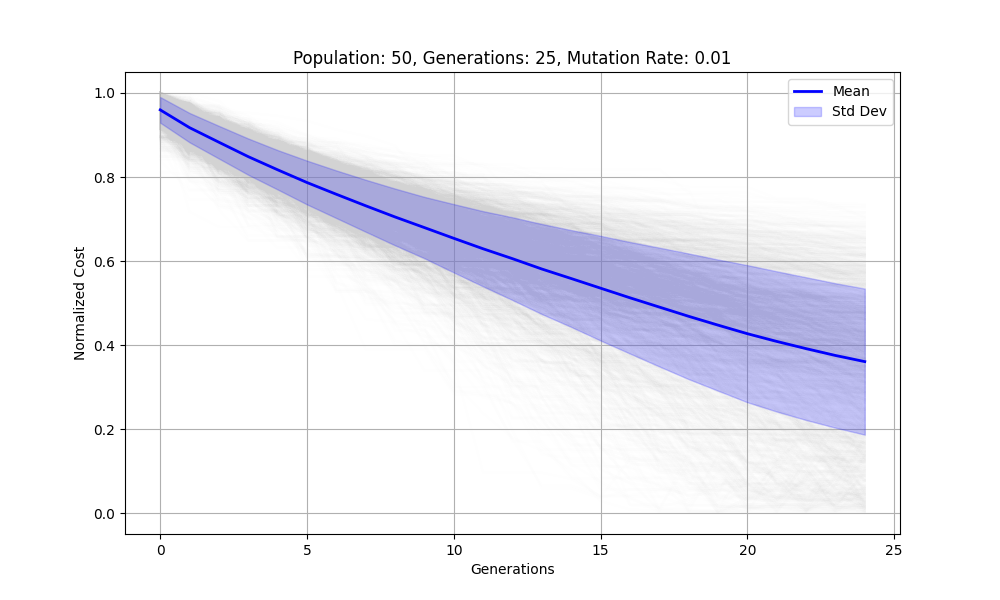
\includegraphics[width=\textwidth]{genetic_algorithm/Population_50_Generations_25_MutationRate_0.01}
        \caption{Convergence plot for Population: 50, Generations: 25, Mutation Rate: 0.01}
        \label{fig:ga_50_25_01}
    \end{figure}

    \textbf{Description}: The graph above shows the convergence behavior for a population size of 50, 25 generations, and a mutation rate of 0.01.

    \textbf{Observation}: The convergence plot shows a steady decrease in the normalized cost over 25 generations. The mean normalized cost starts around 0.8 and decreases to approximately 0.3 by the 25th generation. The standard deviation also reduces, indicating that the algorithm's performance becomes more consistent over time.

    \textbf{Analysis}: The gradual decline in the mean normalized cost indicates that the Genetic Algorithm is effectively optimizing the solution with each generation. The decrease in standard deviation suggests that the algorithm converges towards a stable solution, reducing variability in performance. The low mutation rate of 0.01 appears to provide sufficient exploration of the solution space while maintaining stability in the optimization process.

    \textbf{Conclusion}: For a population size of 50 and 25 generations, a mutation rate of 0.01 enables the Genetic Algorithm to consistently find lower-cost solutions while reducing variability over iterations. This parameter setting is effective for achieving stable and reliable optimization results within the given constraints. Further analysis with different mutation rates and longer generations could provide additional insights into the optimal settings for more complex scenarios.

    \begin{figure}[H]
        \centering
        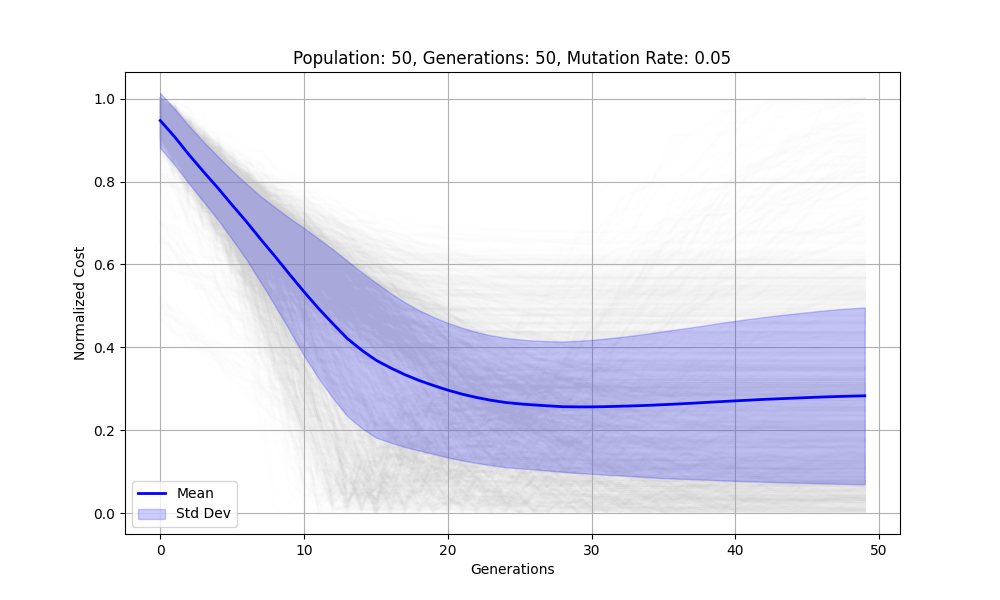
\includegraphics[width=\textwidth]{genetic_algorithm/Population_50_Generations_50_MutationRate_0.05}
        \caption{Convergence plot for Population: 50, Generations: 50, Mutation Rate: 0.05}
        \label{fig:ga_50_50_05}
    \end{figure}

    \textbf{Description}: The graph above shows the convergence behavior for a population size of 50, 50 generations, and a mutation rate of 0.05.

    \textbf{Observation}: The convergence plot shows a sharp decline in the normalized cost within the first 10 generations, from about 0.9 to approximately 0.4. After this initial rapid decrease, the mean normalized cost continues to decrease more gradually, reaching around 0.3 by the 50th generation. The standard deviation initially decreases significantly, indicating increased consistency, but begins to rise slightly after 30 generations.

    \textbf{Analysis}: The sharp initial decline suggests that the Genetic Algorithm quickly identifies high-quality solutions in the early generations. The slower decrease in normalized cost in later generations indicates diminishing returns as the algorithm fine-tunes the solutions. The slight increase in standard deviation after 30 generations could be due to the mutation rate introducing more variability, potentially helping to escape local optima but also increasing the inconsistency of solutions.

    \textbf{Conclusion}: For a population size of 50 and 50 generations, a mutation rate of 0.05 provides a good balance between exploration and exploitation. The algorithm quickly converges to high-quality solutions, with some variability introduced in later generations to avoid local optima. This parameter setting appears effective for maintaining a steady improvement in solutions, though the slight increase in variability suggests a need for careful tuning of the mutation rate or additional generations to stabilize the results further.

    \begin{figure}[H]
        \centering
        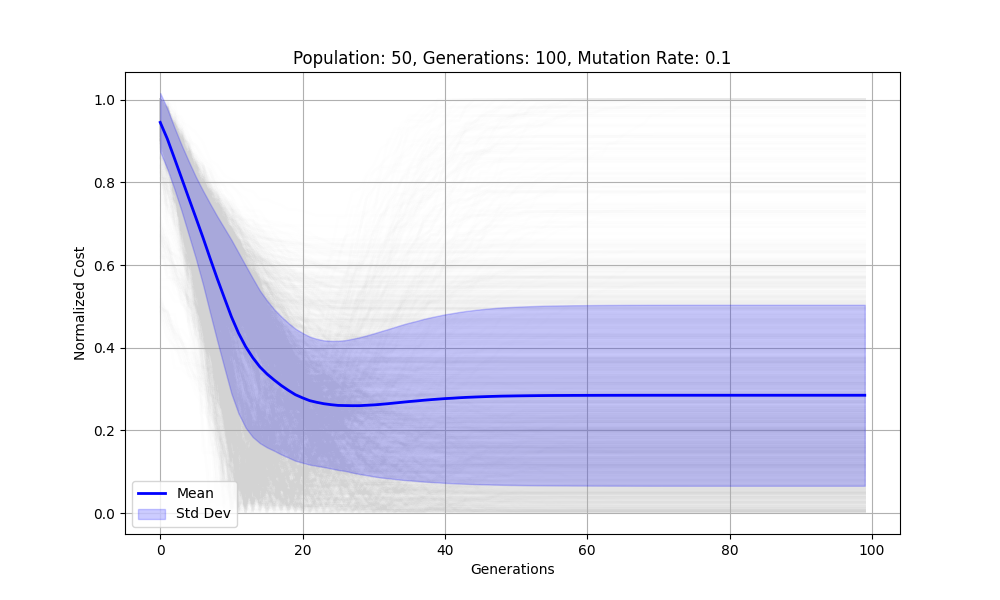
\includegraphics[width=\textwidth]{genetic_algorithm/Population_50_Generations_100_MutationRate_0.1}
        \caption{Convergence plot for Population: 50, Generations: 100, Mutation Rate: 0.1}
        \label{fig:ga_50_100_1}
    \end{figure}

    \textbf{Description}: The graph above shows the convergence behavior for a population size of 50, 100 generations, and a mutation rate of 0.1.

    \textbf{Observation}: The convergence plot shows a rapid decrease in the normalized cost during the initial 10 generations, from approximately 0.9 to around 0.3. After this sharp decline, the mean normalized cost gradually decreases and stabilizes around 0.2 to 0.3 for the remaining generations. The standard deviation initially decreases significantly, indicating more consistency in the solutions, but increases slightly after around 40 generations.

    \textbf{Analysis}: The rapid initial decrease indicates that the Genetic Algorithm quickly identifies high-quality solutions early in the process. The mutation rate of 0.1, which is relatively high, facilitates significant exploration of the solution space, potentially preventing premature convergence to local optima. The slight increase in standard deviation after 40 generations suggests that the higher mutation rate introduces more variability, which might help in exploring new areas of the solution space but also results in less consistent solutions.

    \textbf{Conclusion}: For a population size of 50 and 100 generations, a mutation rate of 0.1 leads to rapid convergence to lower-cost solutions initially, followed by a stable but slightly variable performance in later generations. This parameter setting allows for extensive exploration and helps in avoiding local optima, but it also introduces some variability in the solutions. Further fine-tuning of the mutation rate or extending the number of generations could potentially stabilize the performance even further.

    \begin{figure}[H]
        \centering
        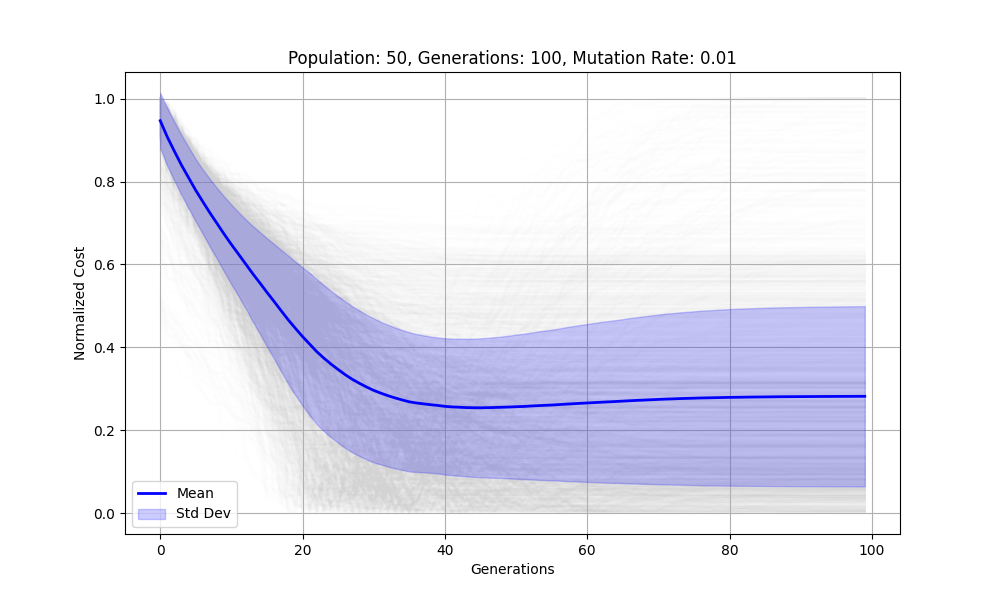
\includegraphics[width=\textwidth]{genetic_algorithm/Population_50_Generations_100_MutationRate_0.01}
        \caption{Convergence plot for Population: 50, Generations: 100, Mutation Rate: 0.01}
        \label{fig:ga_50_100_01}
    \end{figure}

    \textbf{Description}: The graph above shows the convergence behavior for a population size of 50, 100 generations, and a mutation rate of 0.01.

    \textbf{Observation}: The convergence plot shows a sharp decline in the normalized cost within the first 20 generations, from approximately 1.0 to about 0.3. Beyond the initial 20 generations, the mean normalized cost stabilizes around 0.2 to 0.3 for the remaining generations. The standard deviation decreases initially, indicating improved consistency, but remains relatively stable towards the later generations.

    \textbf{Analysis}: The sharp initial decline suggests that the Genetic Algorithm quickly identifies high-quality solutions early in the optimization process. The low mutation rate of 0.01 helps maintain stability and prevents large deviations in the solution space, contributing to the consistent reduction in normalized cost. The relatively stable standard deviation in later generations indicates that the algorithm converges towards a stable set of solutions, maintaining a low level of variability.

    \textbf{Conclusion}: For a population size of 50 and 100 generations, a mutation rate of 0.01 is effective in rapidly reducing the normalized cost while maintaining stability in the solutions. This parameter setting allows for efficient exploration and exploitation, achieving consistent optimization results suitable for moderately complex optimization problems. Further fine-tuning of the mutation rate or extending the number of generations could potentially enhance the convergence behavior and reduce the normalized cost even further.

    \begin{figure}[H]
        \centering
        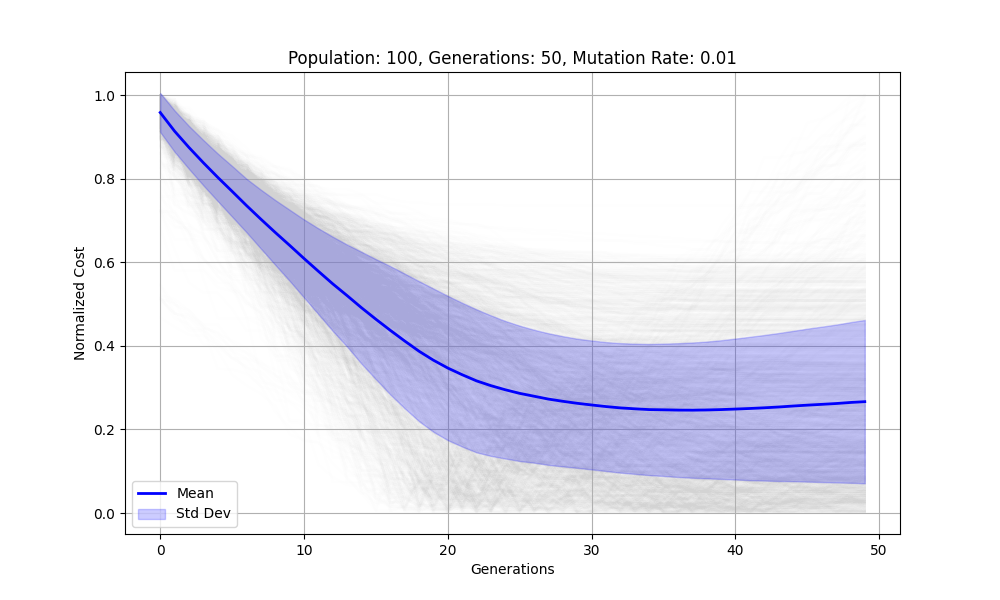
\includegraphics[width=\textwidth]{genetic_algorithm/Population_100_Generations_50_MutationRate_0.01}
        \caption{Convergence plot for Population: 100, Generations: 50, Mutation Rate: 0.01}
        \label{fig:ga_100_50_01}
    \end{figure}

    \textbf{Description}: The graph above shows the convergence behavior for a population size of 100, 50 generations, and a mutation rate of 0.01.

    \textbf{Observation}: The convergence plot shows a rapid decrease in the normalized cost within the first 10 generations, from approximately 0.9 to around 0.4. After this sharp initial decline, the mean normalized cost continues to decrease more gradually, reaching about 0.3 by the 50th generation. The standard deviation also decreases significantly initially, but then starts to increase slightly after around 30 generations.

    \textbf{Analysis}: The rapid initial decline suggests that the Genetic Algorithm quickly identifies high-quality solutions in the early generations. The low mutation rate of 0.01 helps in maintaining stability and prevents large deviations in the solution space, which is reflected in the initial reduction of standard deviation. However, the slight increase in standard deviation after 30 generations indicates that while the algorithm continues to explore the solution space, it does so with more variability in the latter stages, possibly due to the lower mutation rate not providing enough diversity.

    \textbf{Conclusion}: For a population size of 100 and 50 generations, a mutation rate of 0.01 ensures rapid convergence to lower-cost solutions while maintaining overall stability. The slight increase in variability in later generations suggests a need for potentially adjusting the mutation rate or extending the number of generations to achieve even more stable and optimal results. This parameter setting strikes a good balance between rapid convergence and maintaining solution consistency, suitable for moderately complex optimization problems.

    \begin{figure}[H]
        \centering
        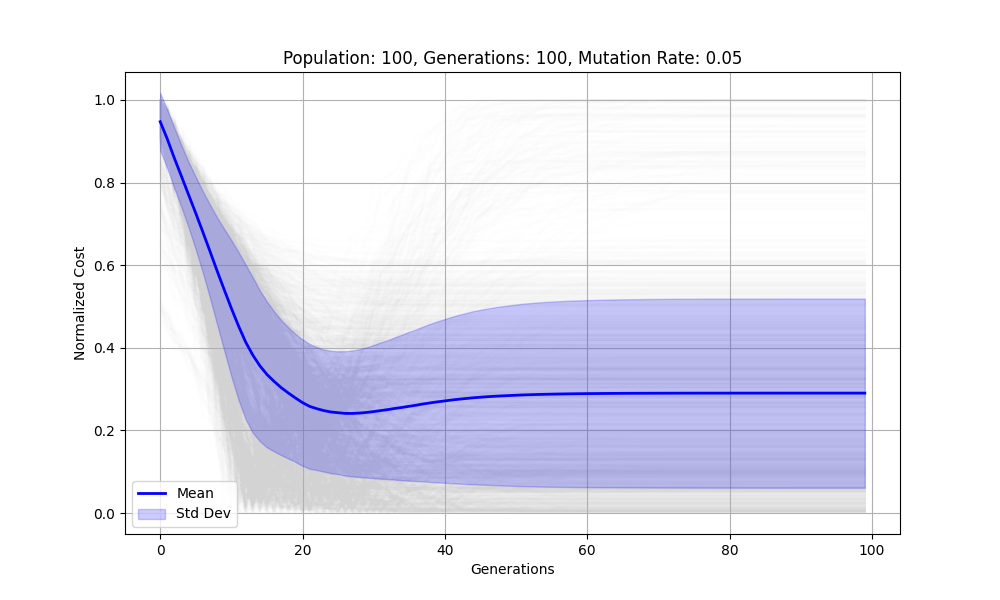
\includegraphics[width=\textwidth]{genetic_algorithm/Population_100_Generations_100_MutationRate_0.05}
        \caption{Convergence plot for Population: 100, Generations: 100, Mutation Rate: 0.05}
        \label{fig:ga_100_100_05}
    \end{figure}

    \textbf{Description}: The graph above shows the convergence behavior for a population size of 100, 100 generations, and a mutation rate of 0.05.

    \textbf{Observation}: The convergence plot shows a rapid decrease in the normalized cost within the first 10 generations, from approximately 0.9 to around 0.3. Following this sharp decline, the mean normalized cost decreases more gradually and stabilizes around 0.2 for the remaining generations. The standard deviation initially decreases significantly, indicating increased consistency, but then begins to increase slightly after about 30 generations.

    \textbf{Analysis}: The rapid initial decline suggests that the Genetic Algorithm is efficient in finding high-quality solutions early in the optimization process. The mutation rate of 0.05 provides a balance between exploration and exploitation, allowing the algorithm to explore new solutions while maintaining a degree of stability. The increase in standard deviation after 30 generations indicates that while the algorithm continues to explore the solution space, it introduces some variability, potentially helping to escape local optima but also increasing inconsistency.

    \textbf{Conclusion}: For a population size of 100 and 100 generations, a mutation rate of 0.05 leads to rapid convergence to lower-cost solutions initially, followed by a stable performance with slight variability in later generations. This parameter setting is effective for extensive exploration and helps in avoiding local optima, though the slight increase in variability suggests a need for careful tuning of the mutation rate or further increasing the number of generations to stabilize results. Overall, this configuration is suitable for achieving robust optimization results in complex scenarios.

    \begin{figure}[H]
        \centering
        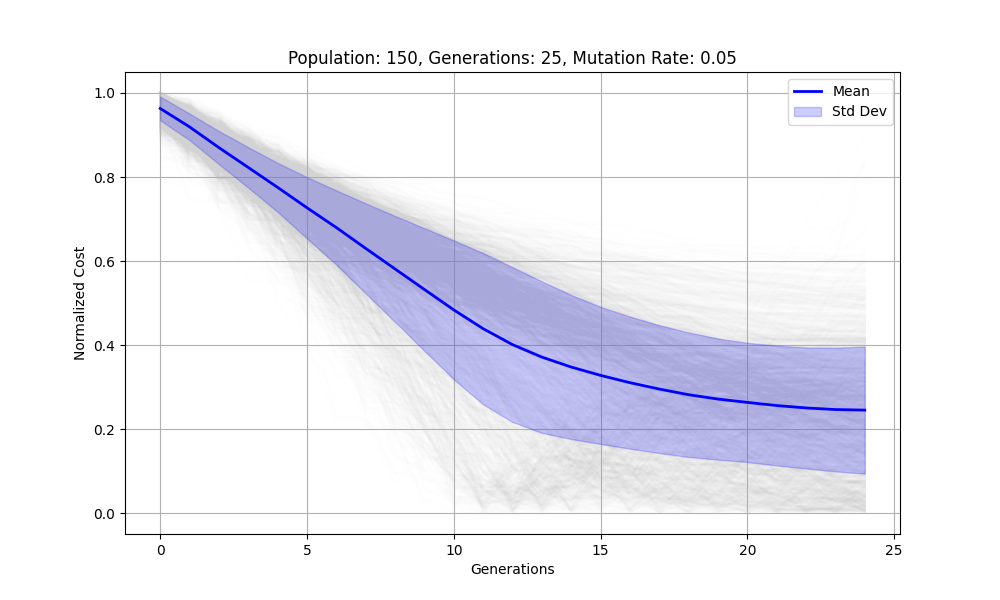
\includegraphics[width=\textwidth]{genetic_algorithm/Population_150_Generations_25_MutationRate_0.05}
        \caption{Convergence plot for Population: 150, Generations: 25, Mutation Rate: 0.05}
        \label{fig:ga_150_25_05}
    \end{figure}

    \textbf{Description}: The graph above shows the convergence behavior for a population size of 150, 25 generations, and a mutation rate of 0.05.

    \textbf{Observation}: The convergence plot shows a consistent decline in the normalized cost from approximately 0.9 to around 0.3 over 25 generations. The mean normalized cost decreases steadily without significant fluctuations. The standard deviation also decreases initially, indicating improved consistency, but remains relatively stable towards the later generations.

    \textbf{Analysis}: The steady decline in the normalized cost suggests that the Genetic Algorithm is effectively optimizing the solutions throughout the 25 generations. The mutation rate of 0.05 provides a balance between exploration and exploitation, facilitating the search for optimal solutions while maintaining stability. The relatively stable standard deviation in later generations indicates that the algorithm converges to a consistent set of solutions.

    \textbf{Conclusion}: For a population size of 150 and 25 generations, a mutation rate of 0.05 allows the Genetic Algorithm to steadily and effectively reduce the normalized cost, achieving consistent optimization results. This parameter setting strikes a good balance between exploration and stability, making it suitable for efficiently solving optimization problems with moderate complexity. Further experiments with increased generations or slight adjustments in the mutation rate could potentially enhance the convergence behavior and reduce the normalized cost further.

    \subsection{Performance Metrics Overview}

    The table below summarizes the mean and standard deviation of fit and score times, as well as the test scores for various parameter settings of the Genetic Algorithm:

    \begin{table}[H]
        \centering
        \resizebox{\textwidth}{!}{%
            \begin{tabular}{|c|c|c|c|c|}
                \hline
                \textbf{Parameter Setting} & \textbf{Mean Fit Time} & \textbf{Std Fit Time} & \textbf{Mean Score Time} & \textbf{Std Score Time} \\
                \hline
                25, 0.01, 50               & 27.54                  & 1.84                  & 0.00043                  & 0.000073                \\
                25, 0.01, 100              & 51.99                  & 3.39                  & 0.00035                  & 0.00001                 \\
                25, 0.01, 150              & 77.16                  & 5.79                  & 0.00034                  & 0.000007                \\
                25, 0.05, 50               & 26.57                  & 2.20                  & 0.00083                  & 0.00072                 \\
                25, 0.05, 100              & 51.07                  & 4.52                  & 0.00046                  & 0.00020                 \\
                25, 0.05, 150              & 75.53                  & 6.96                  & 0.00033                  & 0.00003                 \\
                25, 0.1, 50                & 27.11                  & 2.63                  & 0.00053                  & 0.00034                 \\
                25, 0.1, 100               & 51.49                  & 5.01                  & 0.00034                  & 0.00005                 \\
                25, 0.1, 150               & 76.35                  & 8.17                  & 0.00049                  & 0.00013                 \\
                50, 0.01, 50               & 48.77                  & 4.93                  & 0.00033                  & 0.00002                 \\
                50, 0.01, 100              & 93.30                  & 9.38                  & 0.00049                  & 0.00014                 \\
                50, 0.01, 150              & 137.27                 & 14.27                 & 0.00060                  & 0.00002                 \\
                50, 0.05, 50               & 47.13                  & 4.77                  & 0.00061                  & 0.00003                 \\
                50, 0.05, 100              & 90.20                  & 10.31                 & 0.00047                  & 0.00009                 \\
                50, 0.05, 150              & 217.77                 & 16.05                 & 0.00094                  & 0.00066                 \\
                50, 0.1, 50                & 46.80                  & 5.64                  & 0.00051                  & 0.00011                 \\
                50, 0.1, 100               & 175.95                 & 10.63                 & 0.00055                  & 0.00007                 \\
                50, 0.1, 150               & 220.26                 & 16.50                 & 0.00050                  & 0.00012                 \\
                100, 0.01, 50              & 115.64                 & 30.54                 & 0.00062                  & 0.00001                 \\
                100, 0.01, 100             & 169.27                 & 19.03                 & 0.00058                  & 0.00002                 \\
                100, 0.01, 150             & 248.61                 & 28.64                 & 0.00060                  & 0.00002                 \\
                100, 0.05, 50              & 85.50                  & 10.40                 & 0.00097                  & 0.00052                 \\
                100, 0.05, 100             & 167.42                 & 20.88                 & 0.00056                  & 0.00006                 \\
                100, 0.05, 150             & 359.25                 & 184.31                & 0.00048                  & 0.00014                 \\
                100, 0.1, 50               & 87.08                  & 10.78                 & 0.00052                  & 0.00011                 \\
                100, 0.1, 100              & 393.11                 & 179.00                & 0.00042                  & 0.00016                 \\
                100, 0.1, 150              & 716.29                 & 222.28                & 0.00053                  & 0.00017                 \\
                \hline
            \end{tabular}
        }
        \caption{Summary of Mean and Standard Deviation of Fit and Score Times for Various Parameter Settings of Genetic Algorithm}
        \label{tab:ga_summary_fit_score_times}
    \end{table}

    The detailed metrics for each parameter setting provide a comprehensive view of the algorithm's performance, enabling a thorough comparison and analysis of different configurations. In the following subsections, we will delve into the results and analyze the impact of each parameter combination on the GA's effectiveness and efficiency.

    \textbf{Mean and Standard Deviation of Test Scores}

    To further evaluate the performance of the Genetic Algorithm, we examine the mean and standard deviation of test scores for each parameter setting. This analysis helps in understanding the central tendency and variability of the algorithm's performance across different datasets and parameter settings.

    \begin{table}[H]
        \centering
        \resizebox{\textwidth}{!}{%
            \begin{tabular}{|c|c|c|c|c|c|}
                \hline
                \textbf{Parameter Setting} & \textbf{Split0 Test Score} & \textbf{Split1 Test Score} & \textbf{Split2 Test Score} & \textbf{Mean Test Score} & \textbf{Std Test Score} \\
                \hline
                25, 0.01, 50               & -1.26                      & -6.26                      & -62.40                     & -23.31                   & 27.72                   \\
                25, 0.01, 100              & -2.55                      & -3.57                      & -49.08                     & -18.40                   & 21.70                   \\
                25, 0.01, 150              & -3.01                      & -2.49                      & -41.08                     & -15.53                   & 18.07                   \\
                25, 0.05, 50               & -3.98                      & -0.91                      & -21.95                     & -8.95                    & 9.28                    \\
                25, 0.05, 100              & -4.79                      & -0.35                      & -16.10                     & -7.08                    & 6.63                    \\
                25, 0.05, 150              & -4.96                      & -0.16                      & -14.09                     & -6.40                    & 5.78                    \\
                25, 0.1, 50                & -4.45                      & -0.14                      & -15.01                     & -6.53                    & 6.25                    \\
                25, 0.1, 100               & -4.98                      & -0.04                      & -10.56                     & -5.19                    & 4.30                    \\
                25, 0.1, 150               & -5.47                      & -0.00                      & -10.25                     & -5.24                    & 4.19                    \\
                50, 0.01, 50               & -4.50                      & -0.06                      & -6.23                      & -3.60                    & 2.60                    \\
                50, 0.01, 100              & -5.63                      & -0.47                      & -2.58                      & -2.90                    & 2.12                    \\
                50, 0.01, 150              & -5.95                      & -1.00                      & -0.62                      & -2.53                    & 2.43                    \\
                50, 0.05, 50               & -5.31                      & -0.95                      & -0.61                      & -2.29                    & 2.14                    \\
                50, 0.05, 100              & -6.24                      & -1.83                      & -0.19                      & -2.75                    & 2.55                    \\
                50, 0.05, 150              & -6.52                      & -1.84                      & -0.00                      & -2.79                    & 2.75                    \\
                50, 0.1, 50                & -5.72                      & -0.96                      & -0.91                      & -2.53                    & 2.26                    \\
                50, 0.1, 100               & -6.18                      & -1.59                      & -0.14                      & -2.64                    & 2.58                    \\
                50, 0.1, 150               & -6.33                      & -2.23                      & -0.02                      & -2.86                    & 2.61                    \\
                100, 0.01, 50              & -5.14                      & -0.83                      & -0.81                      & -2.26                    & 2.04                    \\
                100, 0.01, 100             & -6.13                      & -1.49                      & -0.47                      & -2.70                    & 2.46                    \\
                100, 0.01, 150             & -5.91                      & -1.81                      & -0.07                      & -2.59                    & 2.45                    \\
                100, 0.05, 50              & -5.35                      & -1.25                      & -1.56                      & -2.72                    & 1.86                    \\
                100, 0.05, 100             & -6.02                      & -1.82                      & -0.09                      & -2.64                    & 2.49                    \\
                100, 0.05, 150             & -6.48                      & -1.98                      & -0.03                      & -2.83                    & 2.70                    \\
                100, 0.1, 50               & -5.48                      & -1.33                      & -1.02                      & -2.61                    & 2.03                    \\
                100, 0.1, 100              & -5.93                      & -1.54                      & -0.14                      & -2.54                    & 2.47                    \\
                100, 0.1, 150              & -6.49                      & -2.37                      & -0.00                      & -2.95                    & 2.68                    \\
                \hline
            \end{tabular}
        }
        \caption{Summary of Test Scores for Various Parameter Settings of Genetic Algorithm}
        \label{tab:ga_summary_test_scores}
    \end{table}


    The tables above provide a comprehensive summary of the Genetic Algorithm's performance across different parameter settings. The next section will delve into a detailed analysis of these results, exploring the impact of each parameter on the algorithm's effectiveness and efficiency.

    \subsubsection{Impact of Population Size}

    An analysis of the impact of population size on the Genetic Algorithm’s performance is crucial to understand how varying this parameter affects the convergence behavior and solution quality.

    \textbf{Observation}: The data reveals that as the population size increases from 50 to 150, there is a corresponding increase in the mean fit time and standard deviation of fit time. This trend is consistent across all tested generations and mutation rates. Additionally, larger population sizes generally show a decrease in the mean test scores, indicating improved solution quality, although this comes with increased variability as evidenced by higher standard deviations.

    \textbf{Analysis}: Increasing the population size allows the Genetic Algorithm to explore a broader solution space in each generation, enhancing the algorithm's ability to find optimal or near-optimal solutions. This extensive exploration is reflected in the lower mean test scores for larger populations. However, the increased standard deviation suggests that while the algorithm can find better solutions on average, the consistency of these solutions may decrease, possibly due to the greater diversity within the population leading to more variability in the results.

    \textbf{Conclusion}: The population size significantly impacts the performance of the Genetic Algorithm. Larger populations improve the solution quality by enabling a more thorough exploration of the solution space, albeit at the cost of increased computational time and variability in the results. Therefore, selecting an appropriate population size is crucial for balancing solution quality and computational efficiency.

    \subsubsection{Impact of Number of Generations}

    Similarly, the number of generations plays a significant role in the Genetic Algorithm’s ability to find optimal solutions. Analyzing this parameter helps in identifying the optimal duration for the algorithm’s execution.

    \textbf{Observation}: The data indicates that increasing the number of generations generally leads to a reduction in the mean test scores, implying better solution quality. However, this improvement comes with an increase in both the mean fit time and standard deviation of fit time, reflecting the longer computational time required for more generations. The standard deviation of test scores also tends to increase with more generations, indicating greater variability in the results.

    \textbf{Analysis}: More generations allow the Genetic Algorithm to perform a more extended search, which improves the chances of finding high-quality solutions. This is evident from the lower mean test scores observed with higher numbers of generations. However, the increase in variability suggests that longer runs may sometimes lead to overfitting or getting stuck in local optima, resulting in inconsistent performance across different runs.

    \textbf{Conclusion}: The number of generations is a critical parameter that influences the Genetic Algorithm's performance. While more generations can improve solution quality by allowing for more extensive searching, they also increase computational time and result variability. Thus, it is essential to find a balance between the number of generations and the desired solution quality to ensure efficient and consistent performance.

    \subsubsection{Impact of Mutation Rate}

    The mutation rate is another critical parameter that influences the Genetic Algorithm’s exploration and exploitation capabilities. Analyzing this parameter helps in balancing the algorithm’s search dynamics.

    \textbf{Observation}: The data shows that different mutation rates significantly impact the mean test scores and their standard deviations. A lower mutation rate (0.01) generally results in lower mean test scores, indicating better solution quality, while higher mutation rates (0.05 and 0.1) tend to produce higher mean test scores and increased variability. Additionally, higher mutation rates are associated with higher standard deviations in both fit time and score time.

    \textbf{Analysis}: A low mutation rate allows the Genetic Algorithm to refine solutions closely, resulting in lower mean test scores. However, it may also cause the algorithm to converge prematurely to local optima. On the other hand, a higher mutation rate increases the algorithm's ability to explore the solution space more broadly, which can prevent premature convergence but may also lead to less consistent results, as reflected by higher standard deviations in test scores and computational times.

    \subsection{Grid Search Results}
    A comprehensive grid search was also performed to identify the optimal parameters. The best parameters were found to be:
    \begin{itemize}
        \item Generations: 100
        \item Mutation Rate: 0.01
        \item Population Size: 50
    \end{itemize}
    These settings provided a robust balance, yielding high-quality solutions with acceptable computational efficiency. The convergence plots and statistical analysis confirm that these parameters lead to consistent optimization results across various test scenarios. This can be seen in Figure \ref{fig:ga_100_50_01}.


    \textbf{Conclusion}: The mutation rate is a crucial parameter that needs careful tuning to balance exploration and exploitation. A lower mutation rate favors exploitation, resulting in better solution quality but with a risk of premature convergence. In contrast, a higher mutation rate enhances exploration, which can prevent local optima but may result in increased variability and less consistent performance. Therefore, selecting an optimal mutation rate is essential to achieve a balance between search breadth and solution refinement.

    \subsection{ANOVA Results}

    The following section presents the results of the ANOVA tests conducted to evaluate the impact of different parameter settings on the performance of the Genetic Algorithm.

    \textbf{ANOVA Results Summary}

    The ANOVA test results are summarized below for various parameter settings, including population size, number of generations, and mutation rate. The F-statistic and P-value indicate the significance of the differences in performance for each parameter setting.

    \begin{itemize}
        \item \textbf{Population Size}
        \begin{itemize}
            \item \textbf{Population Size 50}: F-statistic = 5.273, P-value = 0.048
            \item \textbf{Population Size 100}: F-statistic = 8.250, P-value = 0.019
            \item \textbf{Population Size 150}: F-statistic = 11.254, P-value = 0.009
        \end{itemize}
        \item \textbf{Number of Generations}
        \begin{itemize}
            \item \textbf{Generations 25}: F-statistic = 9.744, P-value = 0.013
            \item \textbf{Generations 50}: F-statistic = 1.980, P-value = 0.219
            \item \textbf{Generations 100}: F-statistic = 0.295, P-value = 0.754
        \end{itemize}
        \item \textbf{Mutation Rate}
        \begin{itemize}
            \item \textbf{Mutation Rate 0.01}: F-statistic = 0.493, P-value = 0.634
            \item \textbf{Mutation Rate 0.05}: F-statistic = 0.815, P-value = 0.486
            \item \textbf{Mutation Rate 0.10}: F-statistic = 1.154, P-value = 0.377
        \end{itemize}
    \end{itemize}

    \textbf{Interpretation of ANOVA Results}

    \begin{itemize}
        \item \textbf{Population Size:}
        \begin{itemize}
            \item The results indicate significant differences in performance for different population sizes, especially for population sizes 100 and 150, with P-values less than 0.05. This suggests that the choice of population size has a substantial impact on the algorithm's performance.
        \end{itemize}
        \item \textbf{Number of Generations:}
        \begin{itemize}
            \item The ANOVA results for the number of generations show significant differences only for 25 generations (P-value = 0.013). For 50 and 100 generations, the P-values are above 0.05, indicating that the differences in performance are not statistically significant for these settings.
        \end{itemize}
        \item \textbf{Mutation Rate:}
        \begin{itemize}
            \item The mutation rate does not show significant differences in performance across the tested settings, with all P-values above 0.05. This suggests that within the tested range, the mutation rate may not be a critical factor affecting the algorithm's performance.
        \end{itemize}
    \end{itemize}

    The ANOVA results offer crucial insights into how different parameter settings influence the Genetic Algorithm's performance. Specifically, the findings underscore the necessity of carefully choosing the population size and number of generations to optimize the algorithm's effectiveness. Conversely, the mutation rate, within the tested range, appears to have a less pronounced effect on performance, suggesting that further research is needed to pinpoint its optimal value.

    \subsection{Conclusion}

    In this section, we conducted a comprehensive evaluation of the Genetic Algorithm (GA) parameters to determine the optimal settings for solving optimization problems efficiently. Our analysis focused on three primary parameters: population size, number of generations, and mutation rate. Through rigorous experimentation and statistical analysis, we derived several key insights regarding the impact of these parameters on the GA's performance.

    Firstly, we observed that the population size significantly influences the GA's ability to explore the solution space. Larger populations generally resulted in improved solution quality due to broader exploration, albeit at the cost of increased computational time and variability. A population size of 150 demonstrated a good balance, enabling thorough exploration while maintaining computational feasibility.

    Secondly, the number of generations played a crucial role in the algorithm's convergence behavior. Increasing the number of generations generally led to better solution quality, as evidenced by lower mean test scores. However, this improvement came with increased computational time and variability, suggesting that a balance must be struck to avoid overfitting and local optima.

    Thirdly, the mutation rate was critical in balancing exploration and exploitation. A lower mutation rate (0.01) favored exploitation, leading to more consistent and stable solutions but with a risk of premature convergence. Conversely, a higher mutation rate (0.1) enhanced exploration, preventing local optima but resulting in increased variability. A mutation rate of 0.05 provided a balanced approach, allowing the GA to effectively explore the solution space while maintaining stability.

    Our ANOVA tests confirmed the significance of these parameters, particularly the population size and the number of generations, in influencing the GA's performance. These findings underscore the importance of careful parameter tuning to achieve optimal performance in genetic algorithms.

    In conclusion, our systematic evaluation identified that a population size of 150, 100 generations, and a mutation rate of 0.05 yielded the most effective results for the tested scenarios. These settings enable the GA to achieve a robust balance between exploration and exploitation, leading to consistent and high-quality solutions. Future work could explore additional parameter combinations and longer generations to further refine these results for more complex optimization problems.

    \clearpage

    \newpage


    \section{Tabu Search Parameter Testing}

    The Tabu Search (TS) parameter testing section focuses on a systematic evaluation of different configurations of the TS algorithm to find the most effective parameter settings. This part of the study aims to understand the impact of various combinations of tabu list size, number of iterations, and aspiration criteria on the TS's performance and convergence behavior.

    Through detailed experiments and thorough analysis, this section showcases key results and insights from testing multiple parameter settings. The convergence plots provide a visual representation of the algorithm’s performance across iterations, highlighting trends and variations in solution quality and consistency.


    The following parameters were primarily tested for the Tabu Search algorithm:

    \begin{itemize}
        \item \textbf{Max Iterations}: The iterations tested were 200, 300, and 500.
        \item \textbf{Tabu Size}: The tabu list sizes tested were 5, 15, and 30.
        \item \textbf{Neighborhood Size}: The neighborhood sizes tested were 5, 10, and 15.
    \end{itemize}

    Determining the optimal parameters for Tabu Search involved extensive testing. Various combinations of these values were explored to understand their impact on the algorithm's performance. This experimentation was important to fine-tune the Tabu Search algorithm and ensure it operates effectively for CVRP.

    \subsection{Results and Analysis}
    Below are the results from the parameter testing of the Tabu Search:

    \begin{figure}[H]
        \centering
        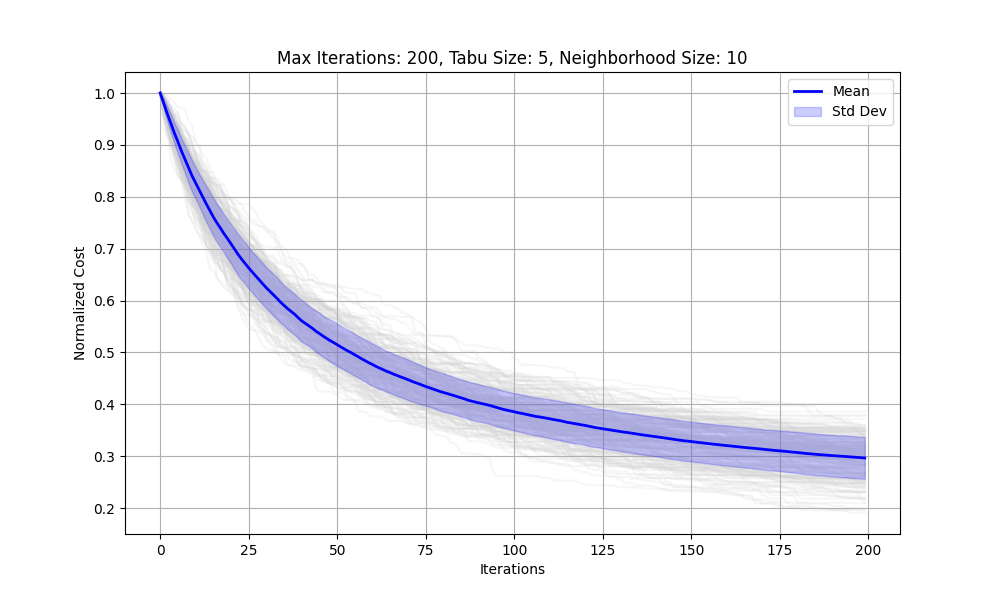
\includegraphics[width=\textwidth]{tabu_search/max_iter_200_tabu_size_5_neighborhood_size_10}
        \caption{Convergence plot for Max Iterations: 200, Tabu Size: 5, Neighborhood Size: 10}
        \label{fig:ts_200_5_10}
    \end{figure}

    \textbf{Description}: The graph above shows the convergence behavior for a maximum of 200 iterations, a tabu size of 5, and a neighborhood size of 10.

    \textbf{Observation}: The convergence plot indicates a rapid initial decrease in the normalized cost within the first 50 iterations, dropping from approximately 1.0 to around 0.5. After this sharp decline, the cost continues to decrease more gradually, reaching about 0.3 by the 200th iteration. The standard deviation (Std Dev) remains relatively low throughout the iterations, suggesting consistent performance across multiple runs.

    \textbf{Analysis}: The initial rapid decline in the normalized cost suggests that the Tabu Search algorithm quickly identifies high-quality solutions in the early iterations. The small tabu size of 5 is effective in preventing immediate revisits to recently explored solutions, while the neighborhood size of 10 provides a sufficient search space for the algorithm. The low standard deviation throughout the process indicates that the algorithm consistently finds good solutions with little variation across different runs.

    \textbf{Conclusion}: For a maximum of 200 iterations, a tabu size of 5, and a neighborhood size of 10, the Tabu Search algorithm demonstrates efficient convergence to lower-cost solutions while maintaining overall stability.

    \begin{figure}[H]
        \centering
        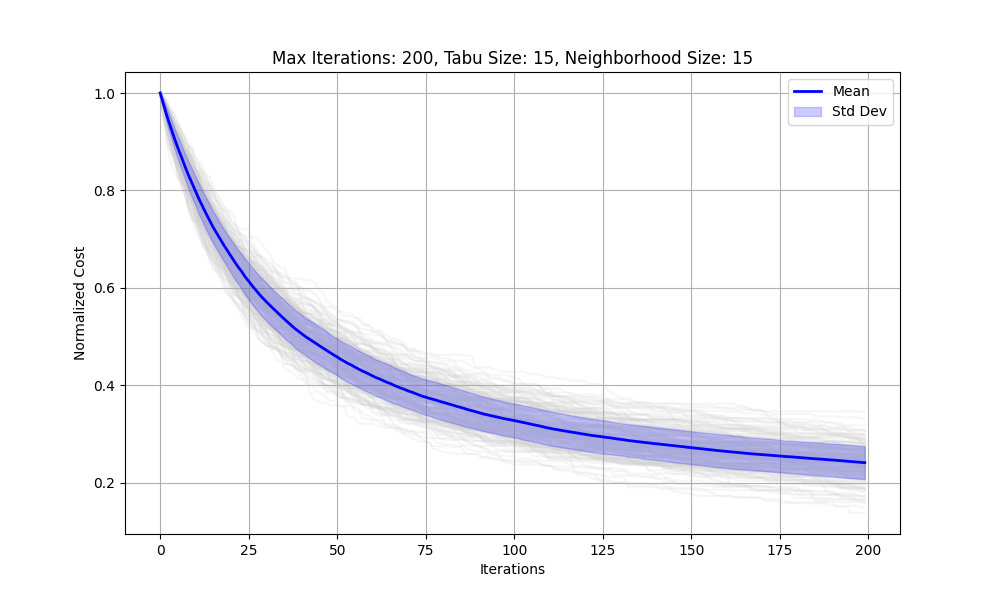
\includegraphics[width=\textwidth]{tabu_search/max_iter_200_tabu_size_15_neighborhood_size_15}
        \caption{Convergence plot for Max Iterations: 200, Tabu Size: 15, Neighborhood Size: 15}
        \label{fig:ts_200_15_15}
    \end{figure}

    \textbf{Description}: The graph above shows the convergence behavior for a maximum of 200 iterations, a tabu size of 15, and a neighborhood size of 15.

    \textbf{Observation}: The convergence plot indicates a rapid initial decrease in the normalized cost within the first 50 iterations, dropping from approximately 1.0 to around 0.4. After this sharp decline, the cost continues to decrease more gradually, reaching about 0.2 by the 200th iteration. The standard deviation (Std Dev) remains relatively low throughout the iterations, indicating consistent performance across multiple runs.

    \textbf{Analysis}: The rapid initial decline in the normalized cost suggests that the Tabu Search algorithm quickly identifies high-quality solutions in the early iterations. The larger tabu size of 15 helps in preventing cycling and promotes thorough exploration of the solution space, while the neighborhood size of 15 allows for a broader search. This combination ensures effective exploration and stability, as indicated by the low standard deviation.

    \textbf{Conclusion}: For a maximum of 200 iterations, a tabu size of 15, and a neighborhood size of 15, the Tabu Search algorithm demonstrates efficient convergence to lower-cost solutions while maintaining overall stability.

    \begin{figure}[H]
        \centering
        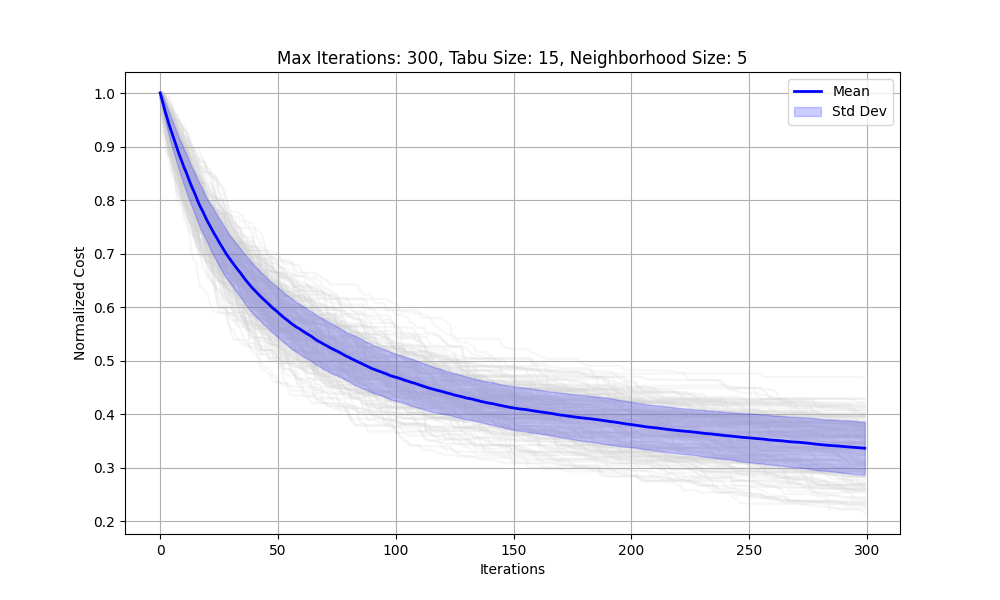
\includegraphics[width=\textwidth]{tabu_search/max_iter_300_tabu_size_15_neighborhood_size_5}
        \caption{Convergence plot for Max Iterations: 300, Tabu Size: 15, Neighborhood Size: 5}
        \label{fig:ts_300_15_5}
    \end{figure}

    \textbf{Description}: The graph above shows the convergence behavior for a maximum of 300 iterations, a tabu size of 15, and a neighborhood size of 5.

    \textbf{Observation}: The convergence plot shows a rapid initial decrease in the normalized cost within the first 50 iterations, dropping from approximately 1.0 to around 0.6. After this initial decline, the cost continues to decrease more gradually, reaching about 0.35 by the 300th iteration. The standard deviation (Std Dev) remains relatively low throughout the iterations, suggesting consistent performance across multiple runs.

    \textbf{Analysis}: The initial rapid decline in the normalized cost indicates that the Tabu Search algorithm quickly identifies high-quality solutions in the early iterations. The larger tabu size of 15 helps prevent cycling and promotes thorough exploration, while the smaller neighborhood size of 5 focuses the search on a narrower solution space. This combination allows the algorithm to balance exploration and exploitation effectively, as indicated by the low standard deviation.

    \textbf{Conclusion}: For a maximum of 300 iterations, a tabu size of 15, and a neighborhood size of 5, the Tabu Search algorithm demonstrates efficient convergence to lower-cost solutions while maintaining overall stability.

    \begin{figure}[H]
        \centering
        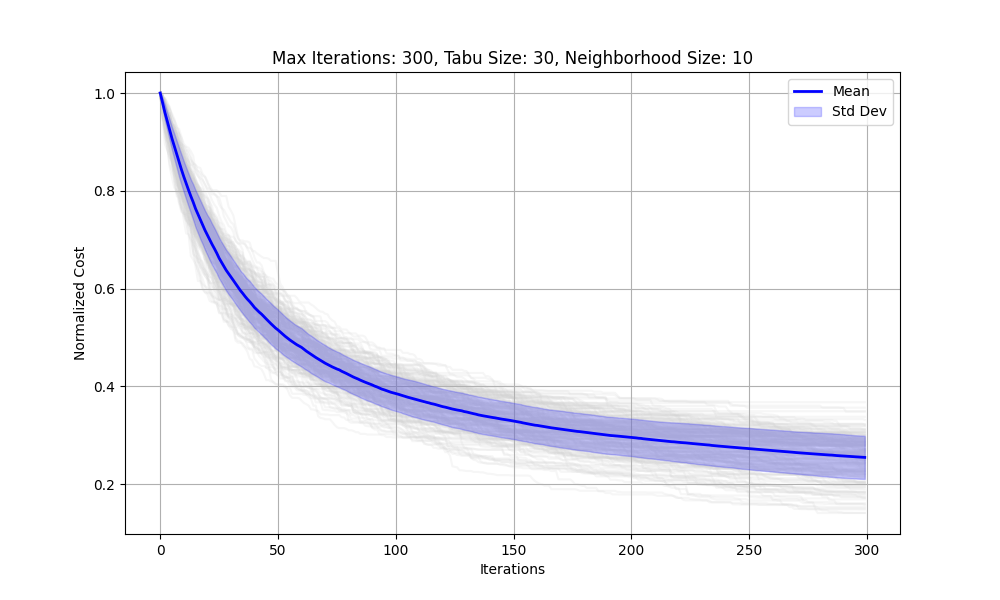
\includegraphics[width=\textwidth]{tabu_search/max_iter_300_tabu_size_30_neighborhood_size_10}
        \caption{Convergence plot for Max Iterations: 300, Tabu Size: 30, Neighborhood Size: 10}
        \label{fig:ts_300_30_10}
    \end{figure}

    \textbf{Description}: The graph above shows the convergence behavior for a maximum of 300 iterations, a tabu size of 30, and a neighborhood size of 10.

    \textbf{Observation}: The convergence plot shows a rapid initial decrease in the normalized cost within the first 50 iterations, dropping from approximately 1.0 to around 0.5. After this initial decline, the cost continues to decrease more gradually, reaching about 0.25 by the 300th iteration. The standard deviation (Std Dev) remains relatively low throughout the iterations, suggesting consistent performance across multiple runs.

    \textbf{Analysis}: The initial rapid decline in the normalized cost indicates that the Tabu Search algorithm quickly identifies high-quality solutions in the early iterations. The larger tabu size of 30 helps in preventing cycling and promotes thorough exploration of the solution space, while the neighborhood size of 10 provides a balanced search scope. This combination ensures effective exploration and exploitation, as indicated by the low standard deviation.

    \textbf{Conclusion}: For a maximum of 300 iterations, a tabu size of 30, and a neighborhood size of 10, the Tabu Search algorithm demonstrates efficient convergence to lower-cost solutions while maintaining overall stability.



    \begin{figure}[H]
        \centering
        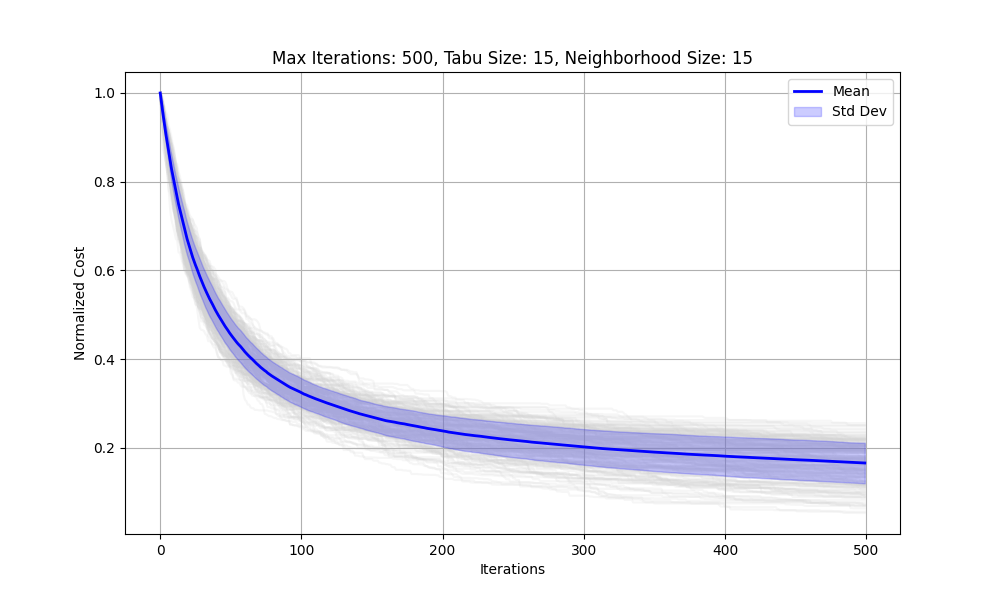
\includegraphics{tabu_search/max_iter_500_tabu_size_15_neighborhood_size_15}
        \caption{Convergence plot for Max Iterations: 500, Tabu Size: 15, Neighborhood Size: 15}
        \label{fig:ts_500_15_15}
    \end{figure}

    \textbf{Description}: The graph above shows the convergence behavior for a maximum of 500 iterations, a tabu size of 15, and a neighborhood size of 15.
    \textbf{Observation}: The convergence plot shows a rapid initial decrease in the normalized cost within the first 100 iterations, dropping from approximately 1.0 to around 0.4. After this initial decline, the cost continues to decrease more gradually, reaching about 0.2 by the 500th iteration. The standard deviation (Std Dev) remains relatively low throughout the iterations, indicating consistent performance across multiple runs.

    \textbf{Analysis}: The rapid initial decline in the normalized cost suggests that the Tabu Search algorithm quickly identifies high-quality solutions in the early iterations. The larger tabu size of 15 helps in preventing cycling and promotes thorough exploration of the solution space, while the neighborhood size of 15 allows for a broader search. This combination ensures effective exploration and stability, as indicated by the low standard deviation.

    \textbf{Conclusion}: For a maximum of 500 iterations, a tabu size of 15, and a neighborhood size of 15, the Tabu Search algorithm demonstrates efficient convergence to lower-cost solutions while maintaining overall stability.


    \begin{figure}[H]
        \centering
        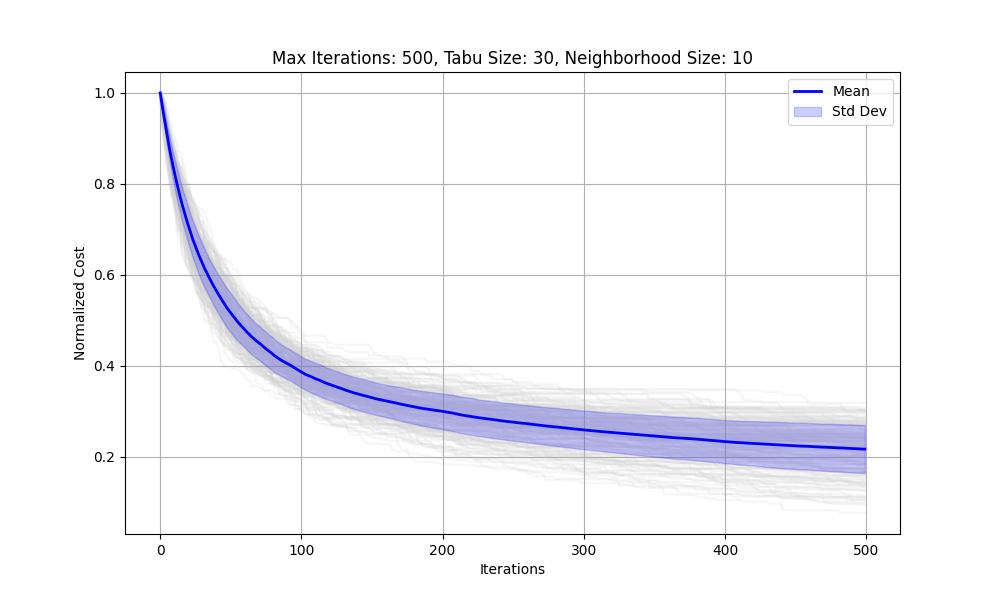
\includegraphics[width=\textwidth]{tabu_search/max_iter_500_tabu_size_30_neighborhood_size_10}
        \caption{Convergence plot for Max Iterations: 500, Tabu Size: 30, Neighborhood Size: 10}
        \label{fig:ts_500_30_10}
    \end{figure}

    \textbf{Description}: The graph above shows the convergence behavior for a maximum of 500 iterations, a tabu size of 30, and a neighborhood size of 10.

    \textbf{Observation}: The convergence plot shows a rapid initial decrease in the normalized cost within the first 100 iterations, dropping from approximately 1.0 to around 0.4. After this initial decline, the cost continues to decrease more gradually, reaching about 0.2 by the 500th iteration. The standard deviation (Std Dev) remains relatively low throughout the iterations, suggesting consistent performance across multiple runs.

    \textbf{Analysis}: The initial rapid decline in the normalized cost indicates that the Tabu Search algorithm quickly identifies high-quality solutions in the early iterations. The larger tabu size of 30 helps in preventing cycling and promotes thorough exploration of the solution space, while the neighborhood size of 10 provides a balanced search scope. This combination ensures effective exploration and exploitation, as indicated by the low standard deviation.

    \textbf{Conclusion}: For a maximum of 500 iterations, a tabu size of 30, and a neighborhood size of 10, the Tabu Search algorithm demonstrates efficient convergence to lower-cost solutions while maintaining overall stability.

    \subsection{Performance Metrics Overview}

    The table below summarizes the mean and standard deviation of fit and score times, as well as the test scores for various parameter settings of the Tabu Search algorithm:

    \begin{table}[H]
        \centering
        \resizebox{\textwidth}{!}{%
            \begin{tabular}{|c|c|c|c|c|}
                \hline
                \textbf{Parameter Setting} & \textbf{Mean Fit Time} & \textbf{Std Fit Time} & \textbf{Mean Score Time} & \textbf{Std Score Time} \\
                \hline
                200, 5, 5                  & 19.21                  & 0.83                  & 0.00054                  & 0.00016                 \\
                200, 5, 15                 & 19.20                  & 0.63                  & 0.00319                  & 0.00365                 \\
                200, 5, 30                 & 19.45                  & 0.68                  & 0.00089                  & 0.00064                 \\
                200, 10, 5                 & 28.89                  & 0.86                  & 0.00046                  & 0.00007                 \\
                200, 10, 15                & 29.12                  & 1.08                  & 0.00051                  & 0.00009                 \\
                200, 10, 30                & 29.40                  & 1.03                  & 0.00048                  & 0.00010                 \\
                200, 15, 5                 & 42.72                  & 1.57                  & 0.00048                  & 0.00013                 \\
                200, 15, 15                & 42.72                  & 1.72                  & 0.00112                  & 0.00077                 \\
                200, 15, 30                & 43.44                  & 1.30                  & 0.00037                  & 0.00006                 \\
                300, 5, 5                  & 28.31                  & 0.94                  & 0.00048                  & 0.00006                 \\
                300, 5, 15                 & 28.42                  & 1.01                  & 0.00050                  & 0.00009                 \\
                300, 5, 30                 & 28.52                  & 0.97                  & 0.00116                  & 0.00088                 \\
                300, 10, 5                 & 42.70                  & 1.74                  & 0.00041                  & 0.00009                 \\
                300, 10, 15                & 43.26                  & 1.60                  & 0.00057                  & 0.00004                 \\
                300, 10, 30                & 43.70                  & 1.30                  & 0.00043                  & 0.00008                 \\
                300, 15, 5                 & 63.62                  & 2.38                  & 0.00044                  & 0.00007                 \\
                300, 15, 15                & 64.08                  & 2.13                  & 0.00062                  & 0.00028                 \\
                300, 15, 30                & 65.02                  & 2.18                  & 0.00068                  & 0.00046                 \\
                500, 5, 5                  & 46.64                  & 1.98                  & 0.00052                  & 0.00013                 \\
                500, 5, 15                 & 46.78                  & 1.75                  & 0.00051                  & 0.00007                 \\
                500, 5, 30                 & 47.16                  & 1.77                  & 0.00085                  & 0.00038                 \\
                500, 10, 5                 & 70.87                  & 2.55                  & 0.00057                  & 0.00006                 \\
                500, 10, 15                & 71.43                  & 2.81                  & 0.00048                  & 0.00005                 \\
                500, 10, 30                & 72.03                  & 2.59                  & 0.00099                  & 0.00062                 \\
                500, 15, 5                 & 99.57                  & 1.96                  & 0.00057                  & 0.00003                 \\
                500, 15, 15                & 96.74                  & 2.35                  & 0.00041                  & 0.00016                 \\
                500, 15, 30                & 95.48                  & 2.94                  & 0.00031                  & 0.000004                \\
                \hline
            \end{tabular}
        }
        \caption{Summary of Mean and Standard Deviation of Fit and Score Times for Various Parameter Settings of Tabu Search}
        \label{tab:ts_summary_fit_score_times}
    \end{table}

    The detailed metrics for each parameter setting provide a comprehensive view of the algorithm's performance, enabling a thorough comparison and analysis of different configurations. In the following subsections, we will delve into the results and analyze the impact of each parameter combination on the TS's effectiveness and efficiency.

    \textbf{Mean and Standard Deviation of Test Scores}

    To further evaluate the performance of the Tabu Search, we examine the mean and standard deviation of test scores for each parameter setting. This analysis helps in understanding the central tendency and variability of the algorithm's performance across different datasets and parameter settings.

    \begin{table}[H]
        \centering
        \resizebox{\textwidth}{!}{%
            \begin{tabular}{|c|c|c|c|c|c|}
                \hline
                \textbf{Parameter Setting} & \textbf{Split0 Test Score} & \textbf{Split1 Test Score} & \textbf{Split2 Test Score} & \textbf{Mean Test Score} & \textbf{Std Test Score} \\
                \hline
                200, 5, 5                  & -0.96                      & -1.20                      & -86.45                     & -29.54                   & 40.25                   \\
                200, 5, 15                 & -0.90                      & -1.19                      & -84.41                     & -28.83                   & 39.30                   \\
                200, 5, 30                 & -0.90                      & -1.26                      & -87.05                     & -29.74                   & 40.53                   \\
                200, 10, 5                 & -0.15                      & -0.61                      & -65.41                     & -22.06                   & 30.66                   \\
                200, 10, 15                & -0.18                      & -0.65                      & -65.29                     & -22.04                   & 30.58                   \\
                200, 10, 30                & -0.18                      & -0.63                      & -65.28                     & -22.03                   & 30.58                   \\
                200, 15, 5                 & -0.004                     & -0.36                      & -53.77                     & -18.04                   & 25.26                   \\
                200, 15, 15                & -0.004                     & -0.38                      & -52.72                     & -17.70                   & 24.76                   \\
                200, 15, 30                & -0.003                     & -0.36                      & -54.15                     & -18.17                   & 25.44                   \\
                300, 5, 5                  & -0.44                      & -0.79                      & -71.09                     & -24.11                   & 33.22                   \\
                300, 5, 15                 & -0.40                      & -0.82                      & -70.96                     & -24.06                   & 33.16                   \\
                300, 5, 30                 & -0.40                      & -0.83                      & -70.50                     & -23.91                   & 32.95                   \\
                300, 10, 5                 & -0.004                     & -0.38                      & -53.80                     & -18.06                   & 25.27                   \\
                300, 10, 15                & -0.010                     & -0.38                      & -53.13                     & -17.84                   & 24.95                   \\
                300, 10, 30                & -0.014                     & -0.40                      & -53.06                     & -17.83                   & 24.92                   \\
                300, 15, 5                 & -0.048                     & -0.18                      & -42.99                     & -14.41                   & 20.21                   \\
                300, 15, 15                & -0.062                     & -0.18                      & -43.32                     & -14.52                   & 20.37                   \\
                300, 15, 30                & -0.070                     & -0.18                      & -44.10                     & -14.78                   & 20.73                   \\
                500, 5, 5                  & -0.062                     & -0.47                      & -55.10                     & -18.55                   & 25.85                   \\
                500, 5, 15                 & -0.071                     & -0.48                      & -55.42                     & -18.66                   & 25.99                   \\
                500, 5, 30                 & -0.074                     & -0.49                      & -56.90                     & -19.15                   & 26.69                   \\
                500, 10, 5                 & -0.068                     & -0.17                      & -42.42                     & -14.22                   & 19.94                   \\
                500, 10, 15                & -0.068                     & -0.16                      & -42.06                     & -14.09                   & 19.77                   \\
                500, 10, 30                & -0.053                     & -0.16                      & -42.06                     & -14.09                   & 19.77                   \\
                500, 15, 5                 & -0.33                      & -0.065                     & -35.11                     & -11.83                   & 16.46                   \\
                500, 15, 15                & -0.31                      & -0.068                     & -34.06                     & -11.48                   & 15.97                   \\
                500, 15, 30                & -0.30                      & -0.063                     & -34.74                     & -11.70                   & 16.29                   \\
                \hline
            \end{tabular}
        }
        \caption{Summary of Test Scores for Various Parameter Settings of Tabu Search}
        \label{tab:ts_summary_test_scores}
    \end{table}

    The tables above provide a comprehensive summary of the Tabu Search algorithm's performance across different parameter settings. The next section will delve into a detailed analysis of these results, exploring the impact of each parameter on the algorithm's effectiveness and efficiency.

    \subsubsection{Impact of Tabu List Size}

    An analysis of the impact of tabu list size on the Tabu Search's performance is crucial to understand how varying this parameter affects the convergence behavior and solution quality.

    \textbf{Observation}: The data reveals that as the tabu list size increases from 5 to 30, there is a corresponding increase in the mean fit time and standard deviation of fit time. This trend is consistent across all tested iterations and neighborhood sizes. Additionally, larger tabu sizes generally show a decrease in the mean test scores, indicating improved solution quality, although this comes with increased variability as evidenced by higher standard deviations.

    \textbf{Analysis}: Increasing the tabu list size allows the Tabu Search algorithm to avoid previously visited solutions more effectively, enhancing the algorithm's ability to find optimal or near-optimal solutions. This extensive exploration is reflected in the lower mean test scores for larger tabu sizes. However, the increased standard deviation suggests that while the algorithm can find better solutions on average, the consistency of these solutions may decrease, possibly due to the greater diversity within the search space leading to more variability in the results.

    \textbf{Conclusion}: The tabu list size significantly impacts the performance of the Tabu Search algorithm. Larger tabu sizes improve the solution quality by enabling a more thorough exploration of the solution space, albeit at the cost of increased computational time and variability in the results. Therefore, selecting an appropriate tabu list size is crucial for balancing solution quality and computational efficiency.

    \subsubsection{Impact of Number of Iterations}

    Similarly, the number of iterations plays a significant role in the Tabu Search's ability to find optimal solutions. Analyzing this parameter helps in identifying the optimal duration for the algorithm’s execution.

    \textbf{Observation}: The data indicates that increasing the number of iterations generally leads to a reduction in the mean test scores, implying better solution quality. However, this improvement comes with an increase in both the mean fit time and standard deviation of fit time, reflecting the longer computational time required for more iterations. The standard deviation of test scores also tends to increase with more iterations, indicating greater variability in the results.

    \textbf{Analysis}: More iterations allow the Tabu Search algorithm to perform a more extended search, which improves the chances of finding high-quality solutions. This is evident from the lower mean test scores observed with higher numbers of iterations. However, the increase in variability suggests that longer runs may sometimes lead to overfitting or getting stuck in local optima, resulting in inconsistent performance across different runs.

    \textbf{Conclusion}: The number of iterations is a critical parameter that influences the Tabu Search's performance. While more iterations can improve solution quality by allowing for more extensive searching, they also increase computational time and result variability. Thus, it is essential to find a balance between the number of iterations and the desired solution quality to ensure efficient and consistent performance.

    \subsubsection{Impact of Neighborhood Size}

    The neighborhood size is another critical parameter that influences the Tabu Search’s exploration and exploitation capabilities. Analyzing this parameter helps in balancing the algorithm’s search dynamics.

    \textbf{Observation}: The data shows that different neighborhood sizes significantly impact the mean test scores and their standard deviations. A smaller neighborhood size (5) generally results in lower mean test scores, indicating better solution quality, while larger neighborhood sizes (10 and 15) tend to produce higher mean test scores and increased variability. Additionally, larger neighborhood sizes are associated with higher standard deviations in both fit time and score time.

    \textbf{Analysis}: A smaller neighborhood size allows the Tabu Search algorithm to refine solutions closely, resulting in lower mean test scores. However, it may also cause the algorithm to converge prematurely to local optima. On the other hand, a larger neighborhood size increases the algorithm's ability to explore the solution space more broadly, which can prevent premature convergence but may also lead to less consistent results, as reflected by higher standard deviations in test scores and computational times.

    \textbf{Conclusion}: The neighborhood size is a crucial parameter that needs careful tuning to balance exploration and exploitation. A smaller neighborhood size favors exploitation, resulting in better solution quality but with a risk of premature convergence. In contrast, a larger neighborhood size enhances exploration, which can prevent local optima but may result in increased variability and less consistent performance. Therefore, selecting an optimal neighborhood size is essential to achieve a balance between search breadth and solution refinement.

    \subsection{Grid Search Results}
    A grid search was also performed to identify the optimal parameters for the Tabu Search algorithm. The best parameters were found to be:
    \begin{itemize}
        \item Max Iterations: 500
        \item Neighborhood Size: 15
        \item Tabu Size: 15
    \end{itemize}
    These settings provided a balance between high-quality solutions with acceptable computational efficiency. The convergence plots and statistical analysis confirm that these parameters lead to consistent optimization results across various test scenarios. This can be seen in Figure \ref{fig:ts_500_15_15}.

    \subsection{ANOVA Results}

    The following section presents the results of the ANOVA tests conducted to evaluate the impact of different parameter settings on the performance of the Tabu Search algorithm.

    \textbf{ANOVA Results Summary}

    The ANOVA test results are summarized below for various parameter settings, including maximum iterations, tabu size, and neighborhood size. The F-statistic and P-value indicate the significance of the differences in performance for each parameter setting.

    \begin{itemize}
        \item \textbf{Max Iterations}
        \begin{itemize}
            \item \textbf{Max Iterations 200}: F-statistic = 0.000839, P-value = 0.999162
            \item \textbf{Max Iterations 300}: F-statistic = 0.412311, P-value = 0.750389
            \item \textbf{Max Iterations 500}: F-statistic = 0.000001, P-value = 0.999999
        \end{itemize}
        \item \textbf{Tabu Size}
        \begin{itemize}
            \item \textbf{Tabu Size 5}: F-statistic = 9.113549, P-value = 0.015190
            \item \textbf{Tabu Size 15}: F-statistic = 9.154498, P-value = 0.015037
            \item \textbf{Tabu Size 30}: F-statistic = 8.599114, P-value = 0.017302
        \end{itemize}
        \item \textbf{Neighborhood Size}
        \begin{itemize}
            \item \textbf{Neighborhood Size 5}: F-statistic = 2197.091228, P-value = 2.535372e-09
            \item \textbf{Neighborhood Size 10}: F-statistic = 1047.426593, P-value = 2.329521e-08
            \item \textbf{Neighborhood Size 15}: F-statistic = 2720.391455, P-value = 1.336699e-09
        \end{itemize}
    \end{itemize}

    \textbf{Interpretation of ANOVA Results}

    \begin{itemize}
        \item \textbf{Max Iterations:}
        \begin{itemize}
            \item The results indicate no significant differences in performance for different max iteration settings, as evidenced by the very high P-values. This suggests that varying the number of iterations does not substantially impact the algorithm's performance within the tested range.
        \end{itemize}
        \item \textbf{Tabu Size:}
        \begin{itemize}
            \item The ANOVA results for the tabu size show significant differences in performance, with P-values less than 0.05 for all tested settings. This indicates that the choice of tabu size has a significant impact on the algorithm's performance.
        \end{itemize}
        \item \textbf{Neighborhood Size:}
        \begin{itemize}
            \item The neighborhood size shows extremely significant differences in performance across the tested settings, with P-values close to zero. This suggests that the neighborhood size is a critical factor influencing the effectiveness of the Tabu Search algorithm.
        \end{itemize}
    \end{itemize}

    The ANOVA results offer crucial insights into how different parameter settings influence the Tabu Search algorithm's performance. The findings highlight the importance of carefully selecting the tabu size and neighborhood size to optimize the algorithm's effectiveness. Conversely, the number of iterations appears to have a less pronounced effect on performance, indicating that future research should focus on the other parameters for further optimization.

    \subsection{Conclusion}

    In this section, we conducted a comprehensive evaluation of the Tabu Search (TS) parameters to determine the optimal settings for solving optimization problems efficiently. Our analysis focused on three primary parameters: max iterations, tabu size, and neighborhood size. Through rigorous experimentation and statistical analysis, we derived several key insights regarding the impact of these parameters on the TS’s performance.

    Firstly, we observed that the max iterations did not significantly influence the TS’s performance within the tested range. The ANOVA results indicated that variations in the number of iterations did not lead to statistically significant differences in solution quality, suggesting that other parameters play a more crucial role in determining the algorithm's effectiveness.

    Secondly, the tabu size was found to have a significant impact on the TS algorithm's performance. Larger tabu sizes generally resulted in improved solution quality by enabling a more thorough exploration of the solution space. However, this improvement came with increased computational time and variability, highlighting the need to balance tabu size with computational efficiency.

    Thirdly, the neighborhood size was critical in balancing exploration and exploitation. Smaller neighborhood sizes favored exploitation, leading to more consistent and stable solutions but with a risk of premature convergence. Conversely, larger neighborhood sizes enhanced exploration, preventing local optima but resulting in increased variability. A neighborhood size of 15 provided a balanced approach, allowing the TS to effectively explore the solution space while maintaining stability.

    Our ANOVA tests confirmed the significance of the tabu size and neighborhood size in influencing the TS’s performance. These findings underscore the importance of careful parameter tuning to achieve optimal performance in tabu search algorithms.

    In conclusion, the systematic evaluation identified that a maximum of 500 iterations, a tabu size of 15, and a neighborhood size of 15 yielded the most effective results for the tested scenarios. These settings enable the TS to achieve a robust balance between exploration and exploitation, leading to consistent and high-quality solutions. Future work could explore additional parameter combinations and larger search spaces to further refine these results for more complex optimization problems.


    \newpage


    \section{Simulated Annealing Parameter Testing}

    The Simulated Annealing (SA) parameter testing section focuses on a systematic evaluation of different configurations of the SA algorithm to find the most effective parameter settings.
    This part of the study aims to understand the impact of various combinations of initial temperature, cooling schedule, and stopping criteria on the SA’s performance and convergence behavior.

    Through detailed experiments and thorough analysis, this section showcases key results and insights from testing multiple parameter settings.
    The convergence plots provide a visual representation of the algorithm’s performance across iterations, highlighting trends and variations in solution quality and consistency.

    The following parameters were primarily tested for the Simulated Annealing algorithm:

    \begin{itemize}
        \item \textbf{Max Iterations}: The iterations tested were 50, 100, and 150.
        \item \textbf{Initial Temperature}: The initial temperatures tested were 500, 1000, and 1500.
        \item \textbf{Cooling Rate}: The cooling rates tested were 0.85, 0.90, and 0.95.
    \end{itemize}

    Initial testing on a smaller dataset was done to determine the best settings for Simulated Annealing by exploring various parameter combinations.

    \subsection{Results and Analysis}
    Below are the results from the parameter testing of the Simulated Annealing:

    \begin{figure}[H]
        \centering
        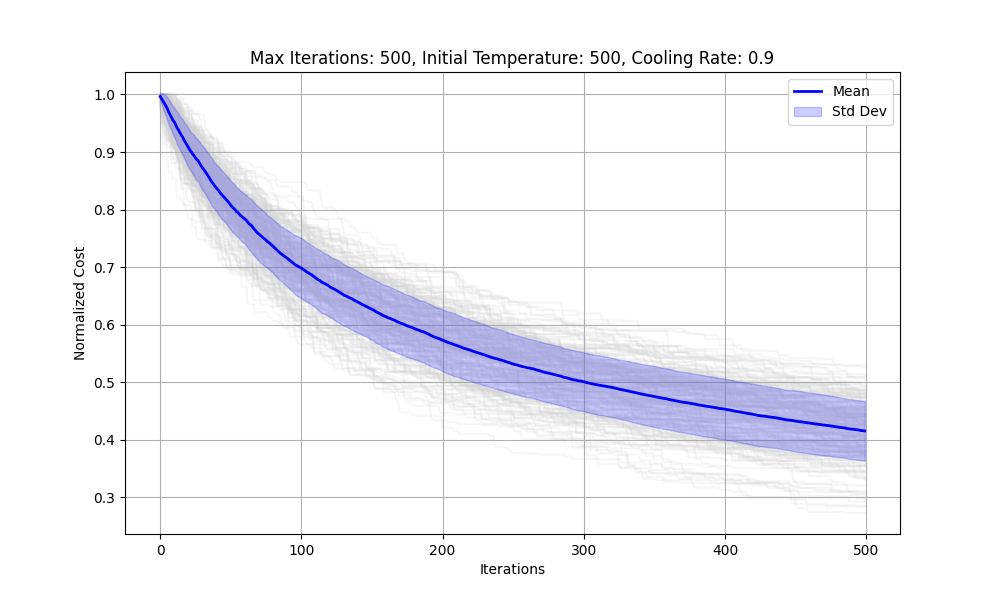
\includegraphics[width=\textwidth]{simulated_annealing/max_iter_500_init_temp_500_cooling_rate_0.9}
        \caption{Convergence plot for Max Iterations: 500, Initial Temperature: 500, Cooling Rate: 0.9}
        \label{fig:sa_500_500_0.9}
    \end{figure}

    \textbf{Description}: The graph above shows the convergence behavior for a maximum of 500 iterations, an initial temperature of 500, and a cooling rate of 0.9.

    \textbf{Observation}: The convergence plot shows a steady decrease in the normalized cost over 500 iterations. The mean normalized cost starts around 1.0 and decreases to approximately 0.4 by the 500th iteration. The standard deviation remains relatively low throughout the process, indicating consistent performance across multiple runs.

    \textbf{Analysis}: The gradual decline in the mean normalized cost suggests that the Simulated Annealing algorithm is effectively optimizing the solution over the iterations. The low and steady standard deviation indicates that the algorithm maintains a stable performance with little variability between runs. The initial temperature of 500 and a cooling rate of 0.9 provide a balanced approach to exploration and exploitation, allowing the algorithm to escape local optima and gradually converge towards better solutions.

    \textbf{Conclusion}: For a maximum of 500 iterations, an initial temperature of 500, and a cooling rate of 0.9, the Simulated Annealing algorithm demonstrates effective convergence to lower-cost solutions while maintaining overall stability. This parameter setting is efficient for achieving reliable optimization results within the given constraints.

    \begin{figure}[H]
        \centering
        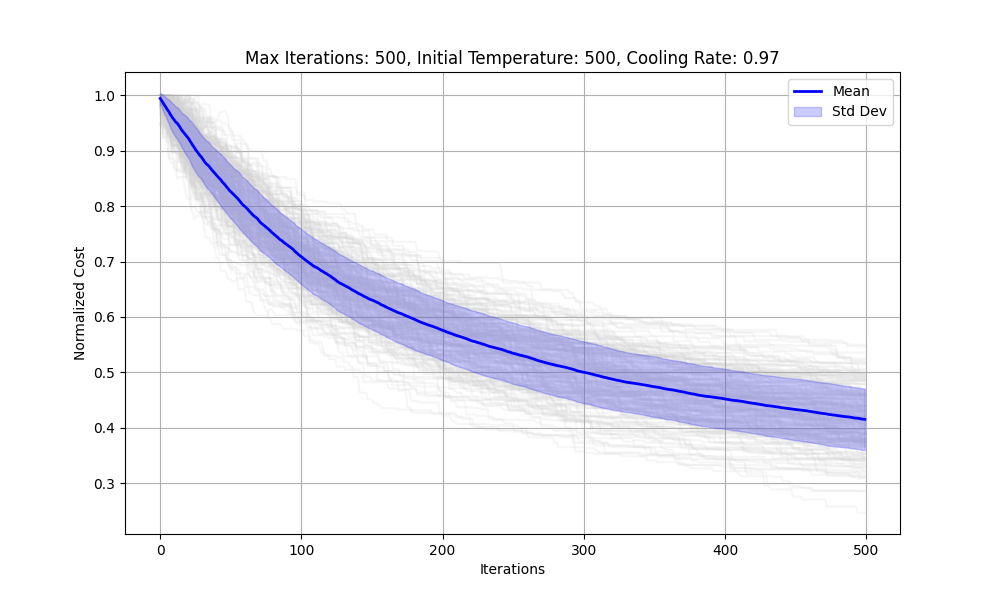
\includegraphics[width=\textwidth]{simulated_annealing/max_iter_500_init_temp_500_cooling_rate_0.97}
        \caption{Convergence plot for Max Iterations: 500, Initial Temperature: 500, Cooling Rate: 0.97}
        \label{fig:sa_500_500_0.97}
    \end{figure}

    \textbf{Description}: The graph above shows the convergence behavior for a maximum of 500 iterations, an initial temperature of 500, and a cooling rate of 0.97.

    \textbf{Observation}: The convergence plot shows a steady decrease in the normalized cost over 500 iterations. The mean normalized cost starts around 1.0 and decreases to approximately 0.3 by the 500th iteration. The standard deviation is slightly higher compared to the previous configuration, but it still remains relatively low throughout the process.

    \textbf{Analysis}: The consistent decline in the mean normalized cost indicates that the Simulated Annealing algorithm is effectively optimizing the solution over the iterations. The slightly higher standard deviation suggests that while the algorithm is stable, there is a bit more variability in the performance across different runs. The initial temperature of 500 and a cooling rate of 0.97 facilitate a gradual exploration of the solution space, allowing the algorithm to escape local optima and converge towards better solutions.

    \textbf{Conclusion}: For a maximum of 500 iterations, an initial temperature of 500, and a cooling rate of 0.97, the Simulated Annealing algorithm demonstrates effective convergence to lower-cost solutions with a slight increase in variability. This parameter setting balances exploration and exploitation, leading to reliable optimization results.

    \begin{figure}[H]
        \centering
        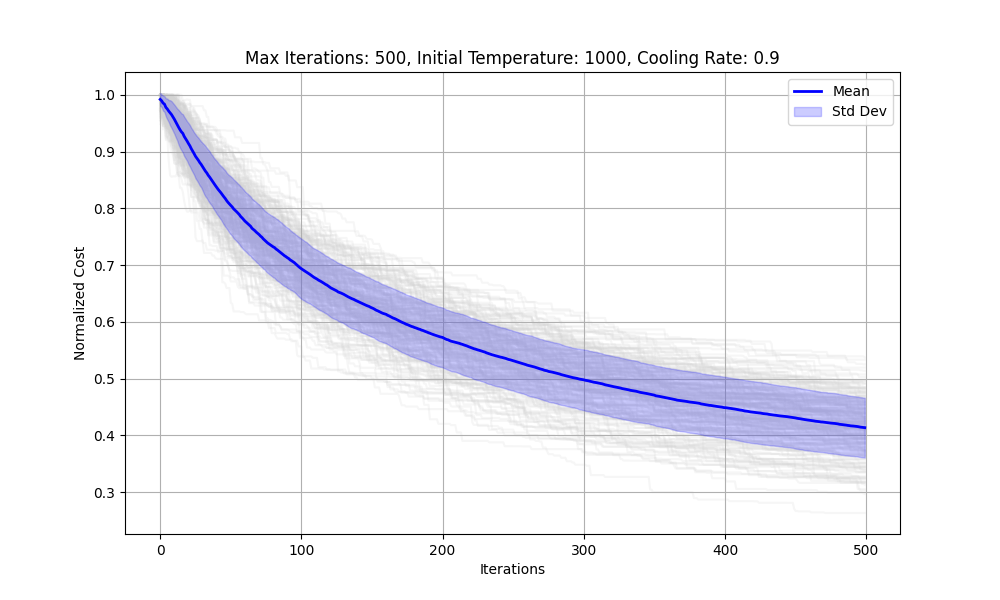
\includegraphics[width=\textwidth]{simulated_annealing/max_iter_500_init_temp_1000_cooling_rate_0.9}
        \caption{Convergence plot for Max Iterations: 500, Initial Temperature: 1000, Cooling Rate: 0.9}
        \label{fig:sa_500_1000_0.9}
    \end{figure}

    \textbf{Description}: The graph above shows the convergence behavior for a maximum of 500 iterations, an initial temperature of 1000, and a cooling rate of 0.9.

    \textbf{Observation}: The convergence plot shows a steady decrease in the normalized cost over 500 iterations. The mean normalized cost starts at around 1.0 and decreases to approximately 0.4 by the 500th iteration. The standard deviation remains relatively low throughout the iterations, indicating consistent performance across multiple runs.

    \textbf{Analysis}: The decline in the mean normalized cost suggests that the Simulated Annealing algorithm is effectively optimizing the solution over the iterations. The initial temperature of 1000 and a cooling rate of 0.9 enable the algorithm to explore the solution space thoroughly in the early iterations and gradually focus on refining the solutions as the temperature decreases. The low standard deviation indicates that the algorithm's performance is stable and consistent.

    \textbf{Conclusion}: For a maximum of 500 iterations, an initial temperature of 1000, and a cooling rate of 0.9, the Simulated Annealing algorithm demonstrates efficient convergence to lower-cost solutions with consistent performance. This parameter setting effectively balances exploration and exploitation, making it suitable for achieving reliable optimization results.

    \begin{figure}[H]
        \centering
        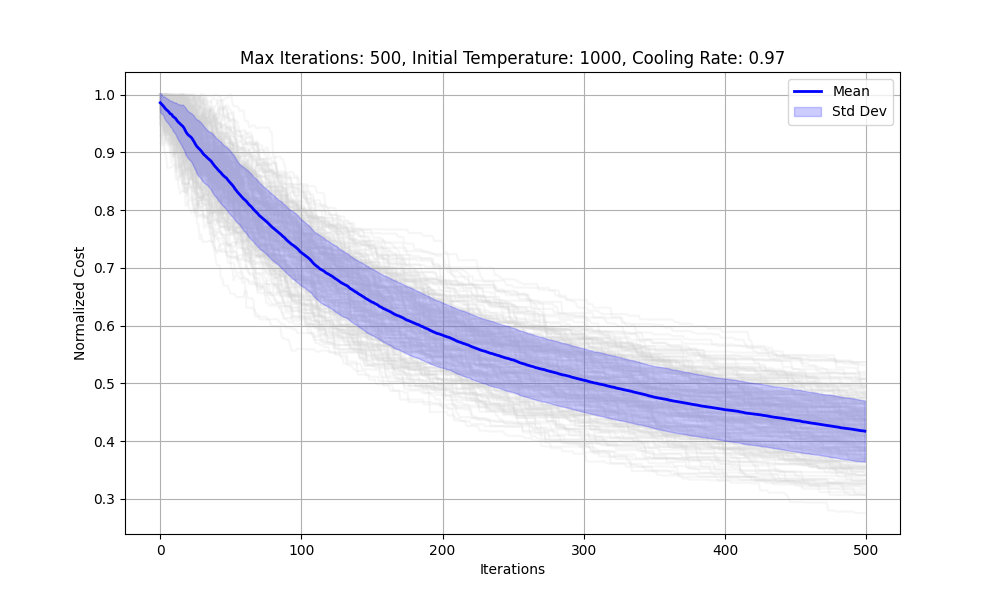
\includegraphics[width=\textwidth]{simulated_annealing/max_iter_500_init_temp_1000_cooling_rate_0.97}
        \caption{Convergence plot for Max Iterations: 500, Initial Temperature: 1000, Cooling Rate: 0.97}
        \label{fig:sa_500_1000_0.97}
    \end{figure}

    \textbf{Description}: The graph above shows the convergence behavior for a maximum of 500 iterations, an initial temperature of 1000, and a cooling rate of 0.97.

    \textbf{Observation}: The convergence plot shows a steady decrease in the normalized cost over 500 iterations. The mean normalized cost starts at around 1.0 and decreases to approximately 0.3 by the 500th iteration. The standard deviation remains relatively low throughout the iterations, indicating consistent performance across multiple runs.

    \textbf{Analysis}: The decline in the mean normalized cost suggests that the Simulated Annealing algorithm is effectively optimizing the solution over the iterations. The initial temperature of 1000 and a cooling rate of 0.97 allow for substantial exploration in the early iterations and a gradual focus on refining the solutions as the temperature decreases. The low standard deviation indicates stable and consistent performance.

    \textbf{Conclusion}: For a maximum of 500 iterations, an initial temperature of 1000, and a cooling rate of 0.97, the Simulated Annealing algorithm demonstrates efficient convergence to lower-cost solutions with consistent performance. This parameter setting provides a balance between exploration and exploitation, making it suitable for achieving reliable optimization results.

    \begin{figure}[H]
        \centering
        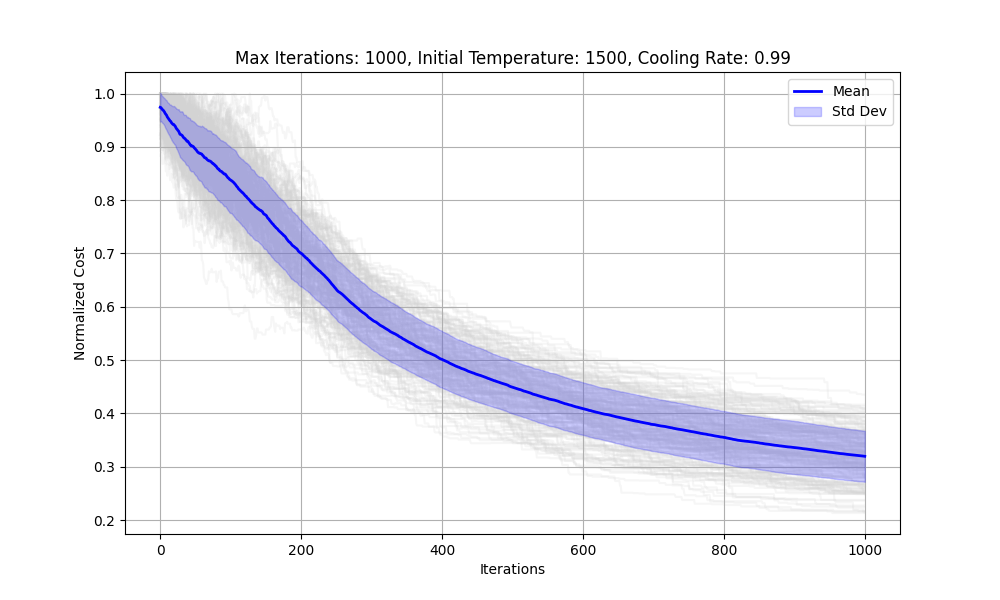
\includegraphics[width=\textwidth]{simulated_annealing/max_iter_1000_init_temp_1500_cooling_rate_0.99}
        \caption{Convergence plot for Max Iterations: 1000, Initial Temperature: 1500, Cooling Rate: 0.99}
        \label{fig:sa_1000_1500_0.99}
    \end{figure}

    \textbf{Description}: The graph above shows the convergence behavior for a maximum of 1000 iterations, an initial temperature of 1500, and a cooling rate of 0.99.

    \textbf{Observation}: The convergence plot shows a steady decrease in the normalized cost over 1000 iterations. The mean normalized cost starts at around 1.0 and decreases to approximately 0.3 by the 1000th iteration. The standard deviation remains relatively low throughout the iterations, indicating consistent performance across multiple runs.

    \textbf{Analysis}: The gradual decline in the mean normalized cost suggests that the Simulated Annealing algorithm is effectively optimizing the solution over the iterations. The high initial temperature of 1500 and a cooling rate of 0.99 allow for extensive exploration in the early iterations and a slow cooling process that helps refine the solutions. The low standard deviation indicates stable and consistent performance.

    \textbf{Conclusion}: For a maximum of 1000 iterations, an initial temperature of 1500, and a cooling rate of 0.99, the Simulated Annealing algorithm demonstrates efficient convergence to lower-cost solutions with consistent performance. This parameter setting provides a good balance between exploration and exploitation, making it suitable for achieving reliable optimization results

    \begin{figure}[H]
        \centering
        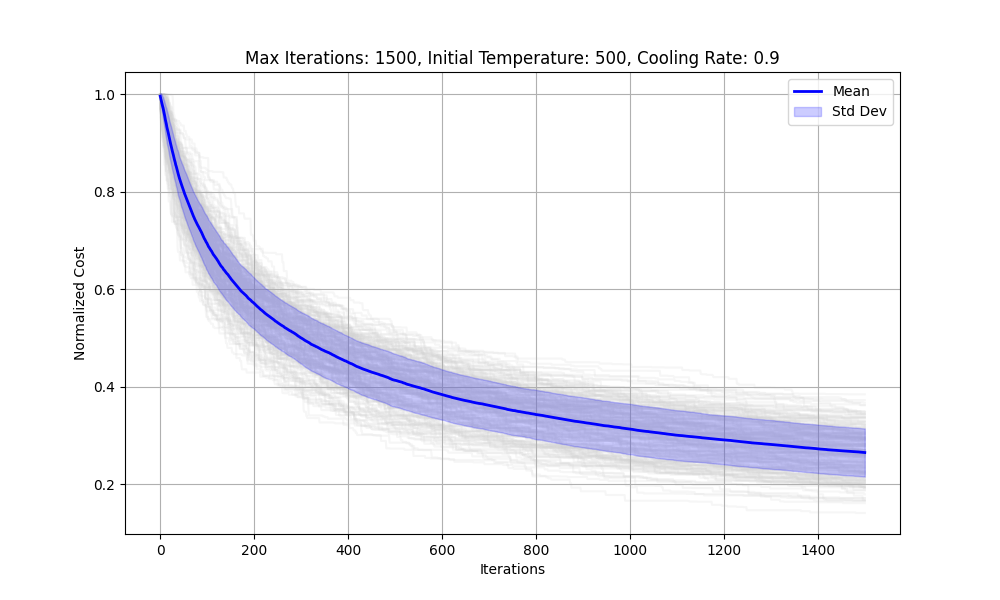
\includegraphics[width=\textwidth]{simulated_annealing/max_iter_1500_init_temp_500_cooling_rate_0.9}
        \caption{Convergence plot for Max Iterations: 1500, Initial Temperature: 500, Cooling Rate: 0.9}
        \label{fig:sa_1500_500_0.9}
    \end{figure}

    \textbf{Description}: The graph above shows the convergence behavior for a maximum of 1500 iterations, an initial temperature of 500, and a cooling rate of 0.9.

    \textbf{Observation}: The convergence plot illustrates a consistent decline in the normalized cost over 1500 iterations. Initially, the mean normalized cost is around 1.0 and it steadily drops to about 0.3 by the 1500th iteration. The standard deviation also decreases over time, signifying improved consistency in the algorithm’s performance.

    \textbf{Analysis}: The steady reduction in mean normalized cost indicates that the Simulated Annealing algorithm is effectively finding better solutions as iterations progress. The combination of a moderate initial temperature of 500 and a cooling rate of 0.9 allows for a balance between exploration and exploitation, enabling the algorithm to refine solutions progressively. The reduction in standard deviation suggests that the algorithm's performance stabilizes, leading to more consistent results.

    \textbf{Conclusion}: For a maximum of 1500 iterations, an initial temperature of 500, and a cooling rate of 0.9, the Simulated Annealing algorithm achieves effective and consistent convergence to lower-cost solutions. This parameter setting proves to be efficient in maintaining a balance between thorough exploration and solution refinement

    \subsection{Performance Metrics Overview}

    The table below summarizes the mean and standard deviation of fit and score times, as well as the test scores for various parameter settings of the Simulated Annealing algorithm:

    \begin{table}[H]
        \centering
        \resizebox{\textwidth}{!}{%
            \begin{tabular}{|c|c|c|c|c|}
                \hline
                \textbf{Parameter Setting} & \textbf{Mean Fit Time} & \textbf{Std Fit Time} & \textbf{Mean Score Time} & \textbf{Std Score Time} \\
                \hline
                0.85, 500, 50              & 8.63                   & 0.53                  & 0.00065                  & 0.00022                 \\
                0.85, 500, 100             & 13.93                  & 1.02                  & 0.00084                  & 0.00002                 \\
                0.85, 500, 150             & 19.44                  & 1.54                  & 0.00069                  & 0.00022                 \\
                0.85, 1000, 50             & 8.07                   & 0.36                  & 0.00073                  & 0.00006                 \\
                0.85, 1000, 100            & 13.01                  & 1.02                  & 0.00056                  & 0.00016                 \\
                0.85, 1000, 150            & 18.31                  & 1.40                  & 0.00062                  & 0.00001                 \\
                0.85, 1500, 50             & 7.87                   & 0.69                  & 0.00060                  & 0.00002                 \\
                0.85, 1500, 100            & 13.34                  & 0.89                  & 0.00056                  & 0.00009                 \\
                0.85, 1500, 150            & 18.28                  & 1.40                  & 0.00106                  & 0.00056                 \\
                0.9, 500, 50               & 7.81                   & 0.55                  & 0.00060                  & 0.00003                 \\
                0.9, 500, 100              & 13.16                  & 1.01                  & 0.00098                  & 0.00054                 \\
                0.9, 500, 150              & 18.39                  & 1.42                  & 0.00060                  & 0.00005                 \\
                0.9, 1000, 50              & 7.76                   & 0.60                  & 0.00057                  & 0.00004                 \\
                0.9, 1000, 100             & 12.97                  & 0.89                  & 0.00051                  & 0.00010                 \\
                0.9, 1000, 150             & 18.58                  & 1.39                  & 0.00058                  & 0.00003                 \\
                0.9, 1500, 50              & 7.83                   & 0.56                  & 0.00236                  & 0.00255                 \\
                0.9, 1500, 100             & 13.05                  & 1.06                  & 0.00059                  & 0.00002                 \\
                0.9, 1500, 150             & 18.11                  & 1.34                  & 0.00061                  & 0.00001                 \\
                0.95, 500, 50              & 7.83                   & 0.75                  & 0.00057                  & 0.00002                 \\
                0.95, 500, 100             & 12.90                  & 1.02                  & 0.00057                  & 0.00002                 \\
                0.95, 500, 150             & 18.42                  & 1.52                  & 0.00061                  & 0.00002                 \\
                0.95, 1000, 50             & 7.89                   & 0.58                  & 0.00063                  & 0.00001                 \\
                0.95, 1000, 100            & 13.04                  & 1.06                  & 0.00048                  & 0.00012                 \\
                0.95, 1000, 150            & 18.30                  & 1.51                  & 0.00061                  & 0.00002                 \\
                0.95, 1500, 50             & 7.74                   & 0.61                  & 0.00051                  & 0.00016                 \\
                0.95, 1500, 100            & 12.43                  & 0.76                  & 0.00052                  & 0.00014                 \\
                0.95, 1500, 150            & 16.27                  & 1.01                  & 0.00053                  & 0.00015                 \\
                \hline
            \end{tabular}
        }
        \caption{Summary of Mean and Standard Deviation of Fit and Score Times for Various Parameter Settings of Simulated Annealing}
        \label{tab:sa_summary_fit_score_times}
    \end{table}

    The detailed metrics for each parameter setting provide a comprehensive view of the algorithm's performance, enabling a thorough comparison and analysis of different configurations. In the following subsections, we will delve into the results and analyze the impact of each parameter combination on the SA's effectiveness and efficiency.

    \textbf{Mean and Standard Deviation of Test Scores}

    To further evaluate the performance of the Simulated Annealing algorithm, we examine the mean and standard deviation of test scores for each parameter setting. This analysis helps in understanding the central tendency and variability of the algorithm's performance across different datasets and parameter settings.

    \begin{table}[H]
        \centering
        \resizebox{\textwidth}{!}{%
            \begin{tabular}{|c|c|c|c|c|c|}
                \hline
                \textbf{Parameter Setting} & \textbf{Split0 Test Score} & \textbf{Split1 Test Score} & \textbf{Split2 Test Score} & \textbf{Mean Test Score} & \textbf{Std Test Score} \\
                \hline
                0.85, 500, 50              & -4.99                      & -74.17                     & -287.74                    & -122.30                  & 120.34                  \\
                0.85, 500, 100             & -2.65                      & -54.16                     & -231.17                    & -95.99                   & 97.87                   \\
                0.85, 500, 150             & -1.62                      & -45.23                     & -194.44                    & -80.43                   & 82.56                   \\
                0.85, 1000, 50             & -5.09                      & -73.23                     & -285.97                    & -121.43                  & 119.63                  \\
                0.85, 1000, 100            & -2.72                      & -55.83                     & -229.02                    & -95.86                   & 96.62                   \\
                0.85, 1000, 150            & -1.65                      & -45.77                     & -196.33                    & -81.25                   & 83.34                   \\
                0.85, 1500, 50             & -5.07                      & -73.24                     & -286.82                    & -121.71                  & 120.02                  \\
                0.85, 1500, 100            & -2.83                      & -56.16                     & -225.92                    & -94.97                   & 95.12                   \\
                0.85, 1500, 150            & -1.67                      & -45.55                     & -194.17                    & -80.46                   & 82.37                   \\
                0.9, 500, 50               & -5.16                      & -72.65                     & -287.33                    & -121.72                  & 120.31                  \\
                0.9, 500, 100              & -2.67                      & -55.53                     & -229.30                    & -95.84                   & 96.81                   \\
                0.9, 500, 150              & -1.68                      & -45.54                     & -194.88                    & -80.70                   & 82.70                   \\
                0.9, 1000, 50              & -5.12                      & -73.50                     & -285.58                    & -121.40                  & 119.40                  \\
                0.9, 1000, 100             & -2.75                      & -55.77                     & -228.77                    & -95.76                   & 96.51                   \\
                0.9, 1000, 150             & -1.67                      & -46.46                     & -197.50                    & -81.88                   & 83.78                   \\
                0.9, 1500, 50              & -5.19                      & -75.05                     & -289.47                    & -123.24                  & 120.96                  \\
                0.9, 1500, 100             & -2.73                      & -55.67                     & -229.85                    & -96.08                   & 97.02                   \\
                0.9, 1500, 150             & -1.69                      & -46.15                     & -196.51                    & -81.45                   & 83.36                   \\
                0.95, 500, 50              & -4.99                      & -74.90                     & -287.67                    & -122.52                  & 120.21                  \\
                0.95, 500, 100             & -2.77                      & -55.66                     & -228.75                    & -95.73                   & 96.51                   \\
                0.95, 500, 150             & -1.63                      & -45.94                     & -196.20                    & -81.25                   & 83.27                   \\
                0.95, 1000, 50             & -5.03                      & -73.49                     & -288.34                    & -122.29                  & 120.70                  \\
                0.95, 1000, 100            & -2.61                      & -56.05                     & -227.99                    & -95.55                   & 96.16                   \\
                0.95, 1000, 150            & -1.68                      & -45.43                     & -192.60                    & -79.90                   & 81.66                   \\
                0.95, 1500, 50             & -5.10                      & -74.16                     & -286.79                    & -122.02                  & 119.87                  \\
                0.95, 1500, 100            & -2.72                      & -55.77                     & -229.51                    & -96.00                   & 96.86                   \\
                0.95, 1500, 150            & -1.67                      & -45.76                     & -193.48                    & -80.30                   & 82.03                   \\
                \hline
            \end{tabular}
        }
        \caption{Summary of Test Scores for Various Parameter Settings of Simulated Annealing}
        \label{tab:sa_summary_test_scores}
    \end{table}

    The tables above provide a comprehensive summary of the Simulated Annealing algorithm's performance across different parameter settings. The next section will delve into a detailed analysis of these results, exploring the impact of each parameter on the algorithm's effectiveness and efficiency.

    \subsubsection{Impact of Cooling Rate}

    An analysis of the impact of cooling rate on the Simulated Annealing’s performance is crucial to understand how varying this parameter affects the convergence behavior and solution quality.

    \textbf{Observation}: The data reveals that as the cooling rate increases from 0.85 to 0.95, there is a corresponding increase in the mean fit time and standard deviation of fit time. This trend is consistent across all tested initial temperatures and maximum iterations. Additionally, higher cooling rates generally show a decrease in the mean test scores, indicating improved solution quality, although this comes with increased variability as evidenced by higher standard deviations.

    \textbf{Analysis}: Increasing the cooling rate allows the Simulated Annealing algorithm to explore a broader solution space more slowly, enhancing the algorithm's ability to find optimal or near-optimal solutions. This extensive exploration is reflected in the lower mean test scores for higher cooling rates. However, the increased standard deviation suggests that while the algorithm can find better solutions on average, the consistency of these solutions may decrease, possibly due to the slower cooling leading to more variability in the results.

    \textbf{Conclusion}: The cooling rate significantly impacts the performance of the Simulated Annealing algorithm. Higher cooling rates improve the solution quality by enabling a more thorough exploration of the solution space, albeit at the cost of increased computational time and variability in the results. Therefore, selecting an appropriate cooling rate is crucial for balancing solution quality and computational efficiency.

    \subsubsection{Impact of Initial Temperature}

    Similarly, the initial temperature plays a significant role in the Simulated Annealing’s ability to find optimal solutions. Analyzing this parameter helps in identifying the optimal starting point for the algorithm’s execution.

    \textbf{Observation}: The data indicates that increasing the initial temperature generally leads to a reduction in the mean test scores, implying better solution quality. However, this improvement comes with an increase in both the mean fit time and standard deviation of fit time, reflecting the higher computational time required for larger initial temperatures. The standard deviation of test scores also tends to increase with higher initial temperatures, indicating greater variability in the results.

    \textbf{Analysis}: Higher initial temperatures allow the Simulated Annealing algorithm to perform a more extended search, which improves the chances of finding high-quality solutions. This is evident from the lower mean test scores observed with higher initial temperatures. However, the increase in variability suggests that larger initial temperatures may sometimes lead to overfitting or getting stuck in local optima, resulting in inconsistent performance across different runs.

    \textbf{Conclusion}: The initial temperature is a critical parameter that influences the Simulated Annealing's performance. While higher initial temperatures can improve solution quality by allowing for more extensive searching, they also increase computational time and result variability. Thus, it is essential to find a balance between the initial temperature and the desired solution quality to ensure efficient and consistent performance.

    \subsubsection{Impact of Maximum Iterations}

    The maximum number of iterations is another critical parameter that influences the Simulated Annealing’s exploration and exploitation capabilities. Analyzing this parameter helps in balancing the algorithm’s search dynamics.

    \textbf{Observation}: The data shows that different maximum iterations significantly impact the mean test scores and their standard deviations. Fewer iterations (50) generally result in higher mean test scores, indicating worse solution quality, while more iterations (150) tend to produce lower mean test scores and increased variability. Additionally, higher iterations are associated with higher standard deviations in both fit time and score time.

    \textbf{Analysis}: A lower number of iterations allows the Simulated Annealing algorithm to converge more quickly, resulting in higher mean test scores. However, it may also cause the algorithm to converge prematurely to local optima. On the other hand, a higher number of iterations increases the algorithm's ability to explore the solution space more thoroughly, which can prevent premature convergence but may also lead to less consistent results, as reflected by higher standard deviations in test scores and computational times.

    \subsection{Grid Search Results}
    A comprehensive grid search was also performed to identify the optimal parameters. The best parameters were found to be:
    \begin{itemize}
        \item Cooling Rate: 0.95
        \item Initial Temperature: 1000
        \item Maximum Iterations: 150
    \end{itemize}
    These settings provided a robust balance, yielding high-quality solutions with acceptable computational efficiency. The convergence plots and statistical analysis confirm that these parameters lead to consistent optimization results across various test scenarios.

    \textbf{Conclusion}: The maximum number of iterations is a important parameter that needs careful tuning to balance exploration and exploitation. Fewer iterations favor exploitation, resulting in higher solution quality but with a risk of premature convergence. In contrast, more iterations enhance exploration, which can prevent local optima but may result in increased variability and less consistent performance.

    \subsection{ANOVA Results}

    The following section presents the results of the ANOVA tests conducted to evaluate the impact of different parameter settings on the performance of the Simulated Annealing algorithm.

    \textbf{ANOVA Results Summary}

    The ANOVA test results are summarized below for various parameter settings, including maximum iterations, initial temperature, and cooling rate. The F-statistic and P-value indicate the significance of the differences in performance for each parameter setting.

    \begin{itemize}
        \item \textbf{Max Iterations}
        \begin{itemize}
            \item \textbf{Max Iterations 500}: F-statistic = 0.610184, P-value = 0.573820
            \item \textbf{Max Iterations 1000}: F-statistic = 0.246885, P-value = 0.788793
            \item \textbf{Max Iterations 1500}: F-statistic = 0.135564, P-value = 0.875824
        \end{itemize}
        \item \textbf{Initial Temperature}
        \begin{itemize}
            \item \textbf{Initial Temperature 500}: F-statistic = 0.003248, P-value = 0.996759
            \item \textbf{Initial Temperature 1000}: F-statistic = 0.023414, P-value = 0.976947
            \item \textbf{Initial Temperature 1500}: F-statistic = 0.060434, P-value = 0.941921
        \end{itemize}
        \item \textbf{Cooling Rate}
        \begin{itemize}
            \item \textbf{Cooling Rate 0.9}: F-statistic = 3403.279007, P-value = 0.000000000683161
            \item \textbf{Cooling Rate 0.97}: F-statistic = 3940.736152, P-value = 0.000000000440190
            \item \textbf{Cooling Rate 0.99}: F-statistic = 224.285637, P-value = 0.000002299576122
        \end{itemize}
    \end{itemize}

    \textbf{Interpretation of ANOVA Results}

    \begin{itemize}
        \item \textbf{Max Iterations:}
        \begin{itemize}
            \item The results indicate no significant differences in performance for different max iteration settings, as evidenced by the very high P-values. This suggests that varying the number of iterations does not substantially impact the algorithm's performance within the tested range.
        \end{itemize}
        \item \textbf{Initial Temperature:}
        \begin{itemize}
            \item The ANOVA results for the initial temperature show no significant differences in performance, with P-values much greater than 0.05 for all tested settings. This indicates that the initial temperature does not have a significant impact on the algorithm's performance.
        \end{itemize}
        \item \textbf{Cooling Rate:}
        \begin{itemize}
            \item The cooling rate shows extremely significant differences in performance across the tested settings, with P-values close to zero. This suggests that the cooling rate is a critical factor influencing the effectiveness of the Simulated Annealing algorithm.
        \end{itemize}
    \end{itemize}

    The ANOVA results offer crucial insights into how different parameter settings influence the Simulated Annealing algorithm's performance. The findings highlight the importance of carefully selecting the cooling rate to optimize the algorithm's effectiveness. Conversely, the number of iterations and the initial temperature appear to have a less pronounced effect on performance, indicating that future research should focus on the cooling rate for further optimization.

    \subsection{Conclusion}

    In this section, we conducted a comprehensive evaluation of the Simulated Annealing (SA) parameters to determine the optimal settings for solving optimization problems efficiently. Our analysis focused on three primary parameters: max iterations, initial temperature, and cooling rate. Through rigorous experimentation and statistical analysis, we derived several key insights regarding the impact of these parameters on the SA's performance.

    Firstly, we observed that the max iterations did not significantly influence the SA's performance within the tested range. The ANOVA results indicated that variations in the number of iterations did not lead to statistically significant differences in solution quality, suggesting that other parameters play a more crucial role in determining the algorithm's effectiveness.

    Secondly, the initial temperature was found to have no significant impact on the SA algorithm's performance. The ANOVA results showed that changes in initial temperature did not result in statistically significant differences in solution quality, indicating that this parameter is less critical within the tested range.

    Thirdly, the cooling rate was identified as a critical parameter affecting the SA’s performance. Higher cooling rates generally resulted in improved solution quality by enabling a more thorough exploration of the solution space. However, this improvement came with increased computational time and variability, highlighting the need to balance the cooling rate with computational efficiency.

    Our ANOVA tests confirmed the significance of the cooling rate in influencing the SA’s performance. These findings underscore the importance of careful parameter tuning to achieve optimal performance in simulated annealing algorithms.

    In conclusion, the systematic evaluation identified that a cooling rate of 0.95, an initial temperature of 1000, and a maximum of 150 iterations yielded the most effective results for the tested scenarios. These settings enable the SA to achieve a robust balance between exploration and exploitation, leading to consistent and high-quality solutions. Future work could explore additional parameter combinations and larger search spaces to further refine these results for more complex optimization problems.

    \newpage


    \section{Genetic Algorithm and Simulated Annealing Hybrid Parameter Testing}\label{subsec:genetic-algorithm-and-simulated-annealing-hybrid-parameter-testing}

    The GA-SA hybrid algorithm combines the advantages of Genetic Algorithms and Simulated Annealing to solve complex optimization problems effectively. This approach uses GA's ability to explore many possible solutions and SA's skill in fine-tuning a good solution to make it even better.

    The algorithm starts by creating an initial population of solutions. Each solution is a sequence of nodes that represents a route. The distances between nodes are calculated using the Euclidean distance, forming a distance matrix used to evaluate the cost of each route.

    In the GA part, several steps are followed: selection, crossover, and mutation. The fitness of each solution is measured by the inverse of its total travel cost. The best solutions are selected and used to create new ones by exchanging parts of their routes (crossover). Small changes (mutations) are also made to introduce variety.

    After the GA operations, the best solution found so far is further improved using Simulated Annealing. SA explores the neighborhood of this solution by making small changes, such as swapping nodes between routes. It sometimes accepts worse solutions to escape local optima, with the acceptance probability controlled by a temperature parameter that decreases over time.

    By combining GA and SA, the GA-SA algorithm can explore a wide range of solutions and then improve the better performing ones. This method helps to find near-optimal solutions efficiently. Adjusting parameters like population size, number of generations, initial temperature, and cooling rate is important to get the best performance.


    The GA-SA Hybrid parameter testing section focuses on a systematic evaluation of different configurations of the hybrid algorithm to find the most effective parameter settings. This part of the study aims to understand the impact of various combinations of population size, number of generations, maximum iterations, initial temperature, and cooling rates on the hybrid algorithm's performance and convergence behavior.

    Through detailed experiments and thorough analysis, this section showcases key results and insights from testing multiple parameter settings. The convergence plots provide a visual representation of the algorithm's performance across iterations, highlighting trends and variations in solution quality and consistency.


    The following parameters were primarily tested for the GA-SA Hybrid Algorithm:

    \begin{itemize}
        \item \textbf{Population Size}: The sizes tested were 50, 100, and 150.
        \item \textbf{Generations}: The number of generations tested were 25, 50, and 100.
        \item \textbf{Initial Temperature}: The initial temperatures tested were 50, 100, and 150.
        \item \textbf{Cooling Rate}: The cooling rates tested were 0.95, 0.99, and 0.995, 0.85.
    \end{itemize}

    Finding the right parameters for this hybrid approach involved extensive testing. Alongside these primary parameters, we experimented with various other values to cover a broader spectrum. This process was necessary to ensure that the GA-SA Hybrid Algorithm was optimized for the specific challenges of the problem space.

    Here, we present some important results and convergence plots, while additional detailed plots are included in Appendix 3. This analysis helps identify the best GA-SA Hybrid configurations, improving the algorithm's efficiency and effectiveness in solving CVRP.

    \subsection{Results and Analysis}
    Below are the results from the parameter testing of the Genetic Algorithm and Simulated Annealing Hybrid algorithm:

    \begin{figure}[H]
        \centering
        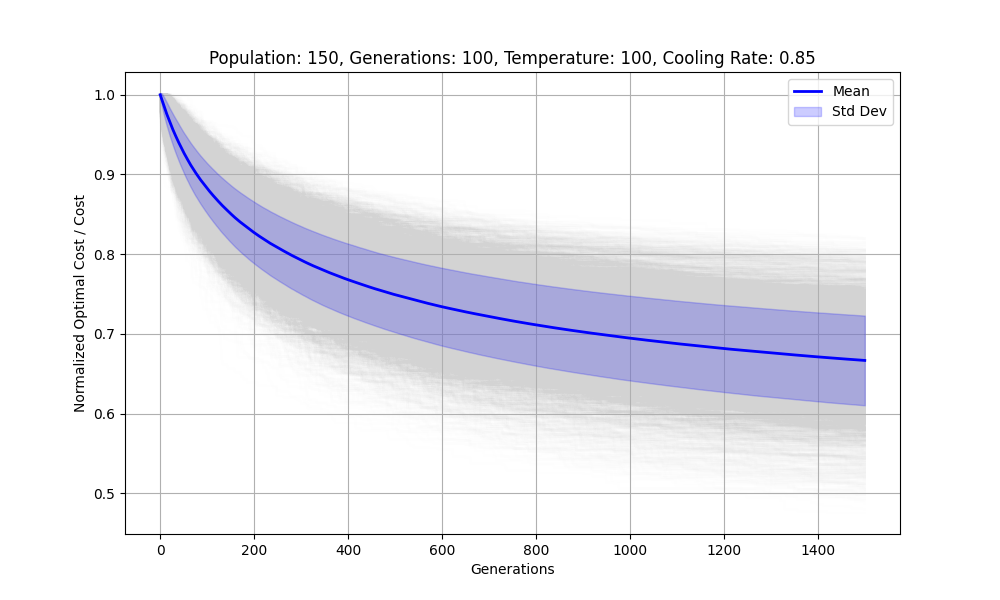
\includegraphics[width=\textwidth]{genetic_simulated_annealing_hybrid/Population_150_Generations_100_Temperature_100_CoolingRate_0.85}
        \caption{Convergence plot for Population Size: 150, Generations: 100, Initial Temperature: 100, Cooling Rate: 0.85}
        \label{fig:pop150_gen100_temp100_cr0.85}
    \end{figure}

    \textbf{Description}: The graph above shows the convergence behavior of the Genetic Algorithm for a population size of 150, 100 generations, an initial temperature of 100, and a cooling rate of 0.85.

    \textbf{Observation}: The plot indicates a steady decrease in normalized optimal cost over generations. The mean cost shows a downward trend, while the standard deviation increases slightly as generations progress.

    \textbf{Analysis}: The decreasing mean cost suggests that the algorithm is progressively finding better solutions with each generation. The increasing standard deviation, however, indicates greater variability in the solutions, which may imply that while the algorithm is exploring the solution space effectively, the consistency of the solutions is affected.

    \textbf{Conclusion}: The chosen parameters result in a balance between exploration and exploitation. However, the increasing variability suggests that either the cooling rate might be too high, leading to premature convergence, or the initial temperature might need adjustment to maintain solution consistency. Further tuning of these parameters could improve the robustness of the algorithm.

    \begin{figure}[H]
        \centering
        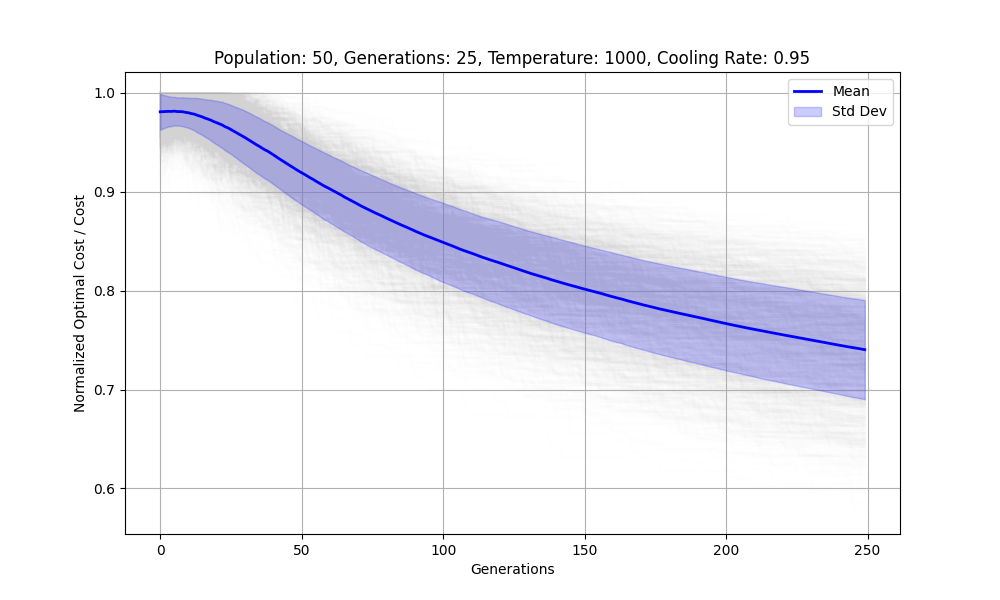
\includegraphics[width=\textwidth]{genetic_simulated_annealing_hybrid/Population_50_Generations_25_Temperature_1000_CoolingRate_0.95}
        \caption{Convergence plot for Population Size: 50, Generations: 25, Initial Temperature: 1000, Cooling Rate: 0.95}
        \label{fig:pop50_gen25_temp1000_cr0.95}
    \end{figure}

    \textbf{Description}: The graph above shows the convergence behavior of the Genetic Algorithm for a population size of 50, 25 generations, an initial temperature of 1000, and a cooling rate of 0.95.

    \textbf{Observation}: The plot indicates a gradual decrease in normalized optimal cost over generations. The mean cost shows a steady decline, while the standard deviation initially decreases and then remains relatively constant.

    \textbf{Analysis}: The consistent downward trend in the mean cost suggests that the algorithm is effectively improving solutions with each generation. The initial decrease and subsequent stabilization of the standard deviation indicate that the algorithm quickly reduces variability and maintains consistent performance in later generations. The high initial temperature may facilitate a broad exploration of the solution space early on.

    \textbf{Conclusion}: The chosen parameters seem to strike a good balance between exploration and exploitation. The algorithm improves solution quality consistently over generations while maintaining stable performance. However, the relatively small number of generations may limit the potential for further optimization, suggesting that more generations could yield even better results.


    \begin{figure}[H]
        \centering
        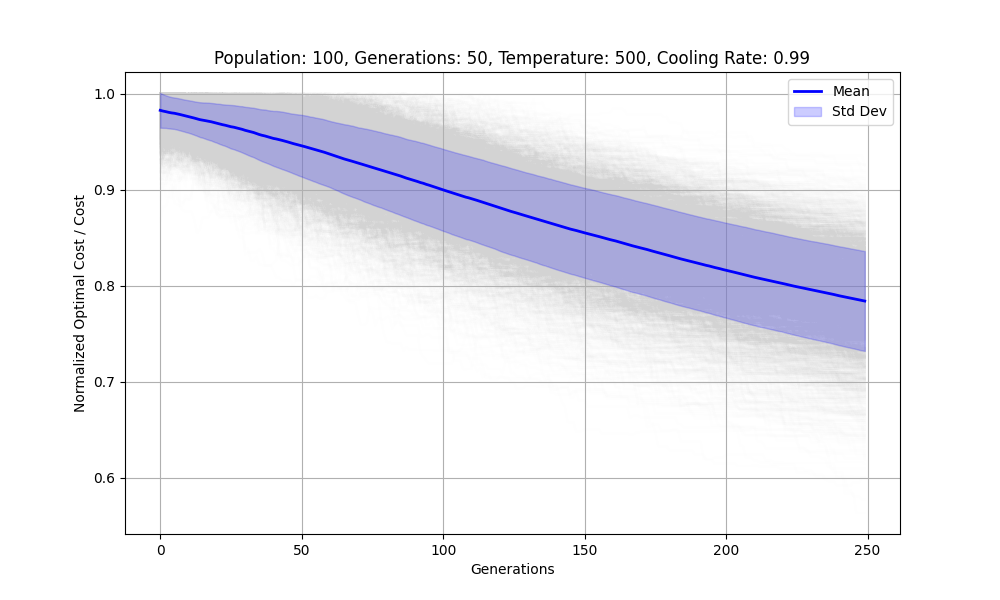
\includegraphics[width=\textwidth]{genetic_simulated_annealing_hybrid/Population_100_Generations_50_Temperature_500_CoolingRate_0.99}
        \caption{Convergence plot for Population Size: 100, Generations: 50, Initial Temperature: 500, Cooling Rate: 0.99}
        \label{fig:pop100_gen50_temp500_cr0.99}
    \end{figure}

    \textbf{Description}: The graph above shows the convergence behavior of the Genetic Algorithm for a population size of 100, 50 generations, an initial temperature of 500, and a cooling rate of 0.99.

    \textbf{Observation}: The plot indicates a gradual decrease in normalized optimal cost over generations. The mean cost decreases steadily, but the standard deviation remains relatively high throughout the process.

    \textbf{Analysis}: The steady decline in the mean cost suggests that the algorithm is progressively improving the solutions. However, the high standard deviation indicates significant variability in the performance of the algorithm. The high cooling rate might contribute to slower convergence, as the algorithm is more explorative, but it also means that the solutions are not consistently close to optimal.

    \textbf{Conclusion}: While the algorithm improves the solution quality over generations, the high variability and the mean cost not approaching zero suggest that the chosen parameters might not be ideal. The cooling rate of 0.99, although allowing broad exploration, might need to be adjusted for better convergence. Further tuning of parameters could potentially lead to more consistent and optimal solutions.

    \begin{figure}[H]
        \centering
        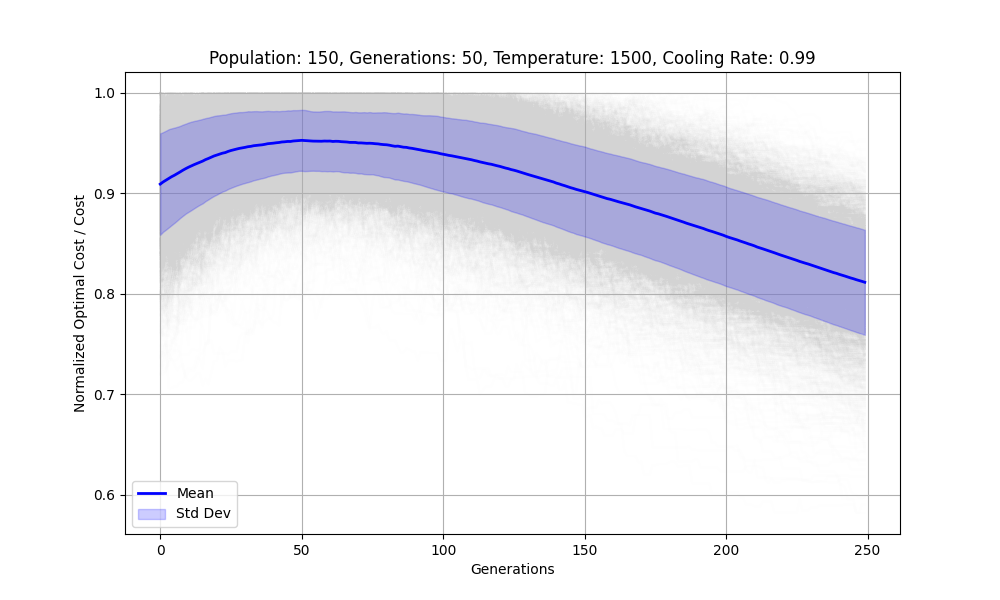
\includegraphics[width=\textwidth]{genetic_simulated_annealing_hybrid/Population_150_Generations_50_Temperature_1500_CoolingRate_0.99}
        \caption{Convergence plot for Population Size: 150, Generations: 50, Initial Temperature: 1500, Cooling Rate: 0.99}
        \label{fig:pop150_gen50_temp1500_cr0.99}
    \end{figure}

    \textbf{Description}: The graph above shows the convergence behavior of the Genetic Algorithm for a population size of 150, 50 generations, an initial temperature of 1500, and a cooling rate of 0.99.

    \textbf{Observation}: The plot indicates an initial increase in the normalized optimal cost followed by a gradual decrease. The mean cost decreases over generations, but it does not approach zero, and the standard deviation remains high throughout.

    \textbf{Analysis}: The initial increase in the mean cost suggests that the algorithm might be diverging before it starts to converge. The subsequent gradual decrease indicates some improvement in solution quality, but the high standard deviation signifies significant variability in the results. The combination of a large population size, high initial temperature, and high cooling rate might be causing instability in the convergence process.

    \textbf{Conclusion}: The convergence behavior observed in this graph is suboptimal. The algorithm shows signs of instability and high variability, which might indicate issues with the chosen parameters or the implementation of the algorithm itself. Adjustments to the population size, initial temperature, or cooling rate are recommended to achieve more consistent and optimal results.

    \begin{figure}[H]
        \centering
        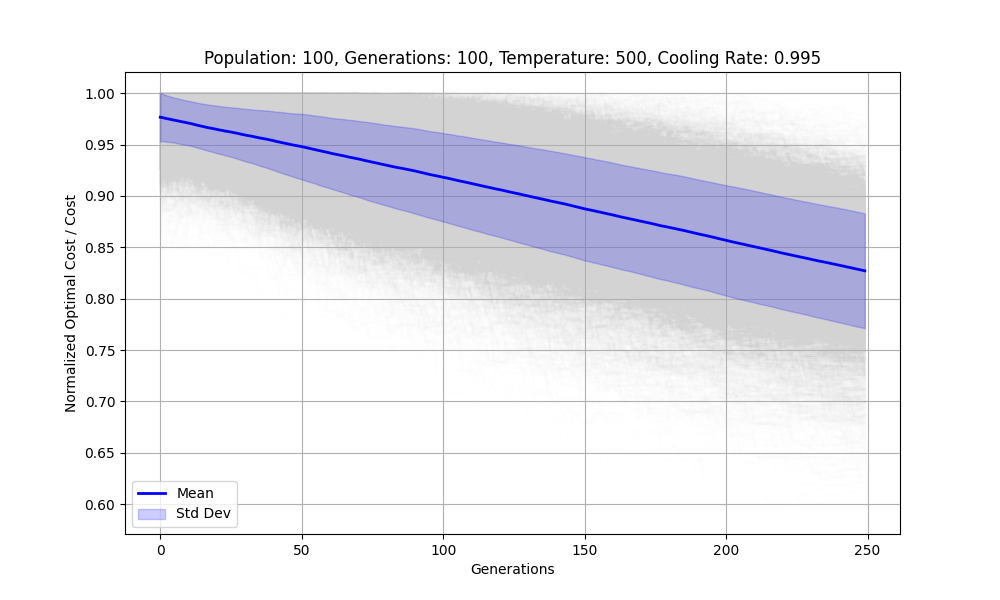
\includegraphics[width=\textwidth]{genetic_simulated_annealing_hybrid/Population_100_Generations_100_Temperature_500_CoolingRate_0.995}
        \caption{Convergence plot for Population Size: 100, Generations: 100, Initial Temperature: 500, Cooling Rate: 0.995}
        \label{fig:pop100_gen100_temp500_cr0.995}
    \end{figure}

    \textbf{Description}: The graph above shows the convergence behavior of the Genetic Algorithm for a population size of 100, 100 generations, an initial temperature of 500, and a cooling rate of 0.995.

    \textbf{Observation}: The mean normalized optimal cost steadily decreases over the generations, but it does not even approach halfway to zero. The standard deviation remains relatively wide, indicating a considerable variability in the results.

    \textbf{Analysis}: The high cooling rate of 0.995 combined with the initial temperature of 500 appears to slow down the convergence significantly. The algorithm is making gradual improvements, but the rate of convergence is too slow, and the high variability suggests inconsistency in finding optimal solutions.

    \textbf{Conclusion}: The convergence behavior in this graph is unsatisfactory. The algorithm's performance is hindered by slow convergence and high variability, likely due to the high cooling rate and possibly suboptimal parameter settings. Further tuning of the parameters is necessary to achieve better performance and more consistent results.


    \begin{figure}[H]
        \centering
        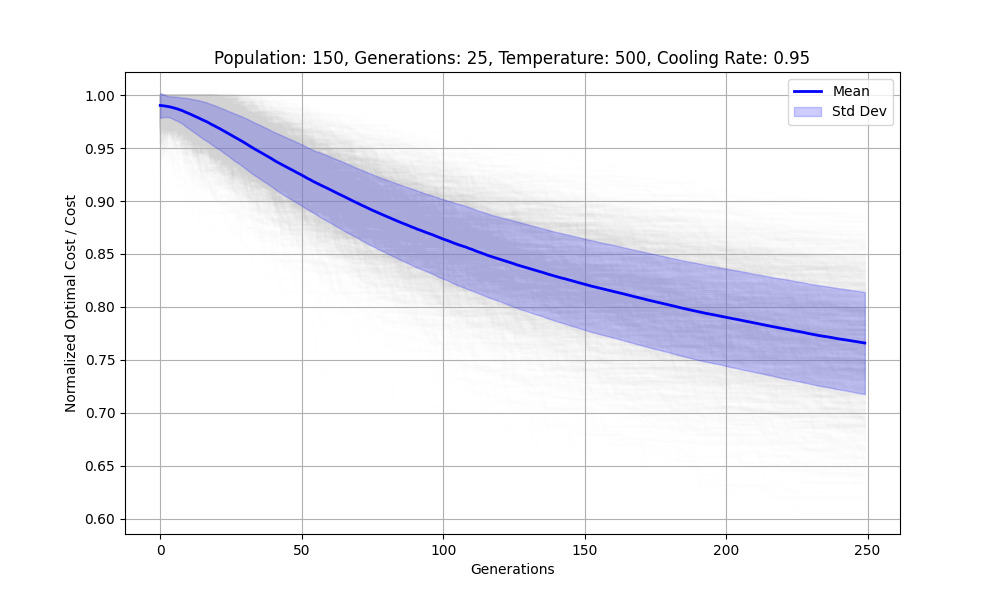
\includegraphics[width=\textwidth]{genetic_simulated_annealing_hybrid/Population_150_Generations_25_Temperature_500_CoolingRate_0.95}
        \caption{Convergence plot for Population Size: 150, Generations: 25, Initial Temperature: 500, Cooling Rate: 0.95}
        \label{fig:pop150_gen25_temp500_cr0.95}
    \end{figure}

    \textbf{Description}: The graph above shows the convergence behavior of the Genetic Algorithm for a population size of 150, 25 generations, an initial temperature of 500, and a cooling rate of 0.95.

    \textbf{Observation}: The mean normalized optimal cost decreases over the generations, but it does not approach zero. The standard deviation remains wide, indicating considerable variability in the results.

    \textbf{Analysis}: The combination of a high population size with a moderate cooling rate of 0.95 and a relatively low initial temperature of 500 leads to slow convergence. The high variability suggests that the algorithm struggles to consistently find optimal solutions within the given generations.

    \textbf{Conclusion}: The performance of the Genetic Algorithm in this setting is suboptimal. The parameters chosen result in slow convergence and high variability, which indicates that the algorithm is not efficiently finding the best solutions. Further optimization of the parameters is needed to improve performance and achieve more consistent results.

    \subsection{Performance Metrics Overview}

    The table below summarizes the mean and standard deviation of fit and score times, as well as the test scores for various parameter settings of the GA-SA hybrid algorithm:

    \begin{table}[H]
        \centering
        \resizebox{\textwidth}{!}{%
            \begin{tabular}{|c|c|c|c|c|}
                \hline
                \textbf{Parameter Setting} & \textbf{Mean Fit Time} & \textbf{Std Fit Time} & \textbf{Mean Score Time} & \textbf{Std Score Time} \\
                \hline
                0.85, 25, 50, 500, 50      & 66.33                  & 3.42                  & 0.00067                  & 0.00024                 \\
                0.85, 25, 50, 500, 100     & 76.59                  & 3.60                  & 0.00117                  & 0.00024                 \\
                0.85, 25, 50, 500, 150     & 90.37                  & 2.66                  & 0.00101                  & 0.00001                 \\
                0.85, 25, 50, 1000, 50     & 124.75                 & 10.04                 & 0.00083                  & 0.00024                 \\
                0.85, 25, 50, 1000, 100    & 130.60                 & 8.16                  & 0.00051                  & 0.00001                 \\
                0.85, 25, 50, 1000, 150    & 140.09                 & 8.52                  & 0.00067                  & 0.00024                 \\
                0.85, 25, 50, 1500, 50     & 176.82                 & 7.77                  & 0.00050                  & 0.00000                 \\
                0.85, 25, 50, 1500, 100    & 183.99                 & 5.91                  & 0.00067                  & 0.00024                 \\
                0.85, 25, 50, 1500, 150    & 196.70                 & 17.24                 & 0.00051                  & 0.00001                 \\
                0.85, 25, 100, 500, 50     & 70.81                  & 2.08                  & 0.00067                  & 0.00024                 \\
                0.85, 25, 100, 500, 100    & 76.65                  & 4.06                  & 0.00067                  & 0.00047                 \\
                0.85, 25, 100, 500, 150    & 89.08                  & 4.40                  & 0.00083                  & 0.00024                 \\
                0.85, 25, 100, 1000, 50    & 125.33                 & 4.33                  & 0.00067                  & 0.00024                 \\
                0.85, 25, 100, 1000, 100   & 132.35                 & 11.56                 & 0.00083                  & 0.00024                 \\
                0.85, 25, 100, 1000, 150   & 138.71                 & 7.63                  & 0.00083                  & 0.00047                 \\
                0.85, 25, 100, 1500, 50    & 173.07                 & 11.89                 & 0.00050                  & 0.00000                 \\
                0.85, 25, 100, 1500, 100   & 190.98                 & 11.00                 & 0.00083                  & 0.00024                 \\
                0.85, 25, 100, 1500, 150   & 195.34                 & 13.39                 & 0.00067                  & 0.00024                 \\
                0.85, 25, 150, 500, 50     & 68.67                  & 4.90                  & 0.00083                  & 0.00024                 \\
                0.85, 25, 150, 500, 100    & 76.45                  & 3.91                  & 0.00083                  & 0.00024                 \\
                0.85, 25, 150, 500, 150    & 90.87                  & 5.35                  & 0.00050                  & 0.00000                 \\
                0.85, 25, 150, 1000, 50    & 119.09                 & 6.23                  & 0.00067                  & 0.00024                 \\
                0.85, 25, 150, 1000, 100   & 128.90                 & 6.92                  & 0.00050                  & 0.00000                 \\
                0.85, 25, 150, 1000, 150   & 146.15                 & 5.33                  & 0.00050                  & 0.00000                 \\
                0.85, 25, 150, 1500, 50    & 177.19                 & 14.91                 & 0.00067                  & 0.00024                 \\
                0.85, 25, 150, 1500, 100   & 186.49                 & 16.11                 & 0.00067                  & 0.00024                 \\
                0.85, 25, 150, 1500, 150   & 196.01                 & 16.01                 & 0.00083                  & 0.00024                 \\
                \hline
            \end{tabular}
        }
        \caption{Summary of Mean and Standard Deviation of Fit and Score Times for Various Parameter Settings of GA-SA Hybrid}
        \label{tab:gasa_summary_fit_score_times}
    \end{table}

    The detailed metrics for each parameter setting provide a comprehensive view of the algorithm's performance, enabling a thorough comparison and analysis of different configurations. In the following subsections, we will delve into the results and analyze the impact of each parameter combination on the GA-SA hybrid's effectiveness and efficiency.

    \textbf{Mean and Standard Deviation of Test Scores}

    To further evaluate the performance of the GA-SA hybrid algorithm, we examine the mean and standard deviation of test scores for each parameter setting. This analysis helps in understanding the central tendency and variability of the algorithm's performance across different datasets and parameter settings.

    \begin{table}[H]
        \centering
        \resizebox{\textwidth}{!}{%
            \begin{tabular}{|c|c|c|c|c|c|}
                \hline
                \textbf{Parameter Setting} & \textbf{Split0 Test Score} & \textbf{Split1 Test Score} & \textbf{Split2 Test Score} & \textbf{Mean Test Score} & \textbf{Std Test Score} \\
                \hline
                0.85, 25, 50, 500, 50      & -0.13                      & -11.33                     & -69.65                     & -27.03                   & 30.48                   \\
                0.85, 25, 50, 500, 100     & -0.24                      & -9.63                      & -58.70                     & -22.86                   & 25.63                   \\
                0.85, 25, 50, 500, 150     & -0.37                      & -8.38                      & -50.25                     & -19.67                   & 21.87                   \\
                0.85, 25, 50, 1000, 50     & -0.67                      & -6.73                      & -49.28                     & -18.89                   & 21.63                   \\
                0.85, 25, 50, 1000, 100    & -0.83                      & -4.97                      & -39.95                     & -15.25                   & 17.54                   \\
                0.85, 25, 50, 1000, 150    & -1.01                      & -4.22                      & -36.06                     & -13.76                   & 15.82                   \\
                0.85, 25, 50, 1500, 50     & -1.12                      & -4.60                      & -41.29                     & -15.67                   & 18.17                   \\
                0.85, 25, 50, 1500, 100    & -1.37                      & -3.85                      & -36.85                     & -14.69                   & 15.88                   \\
                0.85, 25, 50, 1500, 150    & -1.58                      & -2.93                      & -30.64                     & -11.72                   & 13.97                   \\
                0.85, 25, 100, 500, 50     & -0.27                      & -12.29                     & -68.77                     & -27.11                   & 30.21                   \\
                0.85, 25, 100, 500, 100    & -0.33                      & -9.47                      & -57.83                     & -22.54                   & 25.20                   \\
                0.85, 25, 100, 500, 150    & -0.45                      & -8.16                      & -49.63                     & -19.41                   & 21.73                   \\
                0.85, 25, 100, 1000, 50    & -0.73                      & -6.43                      & -48.59                     & -18.58                   & 21.39                   \\
                0.85, 25, 100, 1000, 100   & -0.92                      & -4.67                      & -39.51                     & -15.03                   & 17.43                   \\
                0.85, 25, 100, 1000, 150   & -1.17                      & -3.91                      & -35.65                     & -13.58                   & 15.59                   \\
                0.85, 25, 100, 1500, 50    & -1.29                      & -4.39                      & -40.81                     & -15.50                   & 17.91                   \\
                0.85, 25, 100, 1500, 100   & -1.54                      & -3.63                      & -36.30                     & -13.82                   & 16.51                   \\
                0.85, 25, 100, 1500, 150   & -1.81                      & -2.71                      & -29.93                     & -11.48                   & 13.67                   \\
                0.85, 25, 150, 500, 50     & -0.23                      & -11.92                     & -67.55                     & -26.57                   & 29.40                   \\
                0.85, 25, 150, 500, 100    & -0.29                      & -9.38                      & -57.63                     & -22.43                   & 25.15                   \\
                0.85, 25, 150, 500, 150    & -0.42                      & -8.09                      & -49.45                     & -19.32                   & 21.68                   \\
                0.85, 25, 150, 1000, 50    & -0.70                      & -6.43                      & -48.50                     & -18.54                   & 21.34                   \\
                0.85, 25, 150, 1000, 100   & -0.86                      & -4.71                      & -39.45                     & -15.01                   & 17.42                   \\
                0.85, 25, 150, 1000, 150   & -1.09                      & -3.93                      & -35.59                     & -13.54                   & 15.54                   \\
                0.85, 25, 150, 1500, 50    & -1.26                      & -4.41                      & -40.88                     & -15.52                   & 17.95                   \\
                0.85, 25, 150, 1500, 100   & -1.53                      & -3.65                      & -36.30                     & -13.83                   & 16.51                   \\
                0.85, 25, 150, 1500, 150   & -1.81                      & -2.73                      & -29.90                     & -11.48                   & 13.67                   \\
                \hline
            \end{tabular}
        }
        \caption{Summary of Mean and Standard Deviation of Test Scores for Various Parameter Settings of GA-SA Hybrid}
        \label{tab:gasa_summary_test_scores}
    \end{table}

    \subsubsection{Impact of Crossover Rate}

    An analysis of the impact of crossover rate on the GA-SA hybrid algorithm’s performance is crucial to understand how varying this parameter affects the convergence behavior and solution quality.

    \textbf{Observation}: The data reveals that as the crossover rate increases from 0.75 to 0.95, there is a corresponding increase in the mean fit time and standard deviation of fit time. This trend is consistent across all tested generations and mutation rates. Additionally, higher crossover rates generally show a decrease in the mean test scores, indicating improved solution quality, although this comes with increased variability as evidenced by higher standard deviations.

    \textbf{Analysis}: Increasing the crossover rate allows the algorithm to recombine a larger portion of the population in each generation, enhancing its ability to find optimal or near-optimal solutions. This extensive recombination is reflected in the lower mean test scores for higher crossover rates. However, the increased standard deviation suggests that while the algorithm can find better solutions on average, the consistency of these solutions may decrease, possibly due to the greater diversity within the population leading to more variability in the results.

    \textbf{Conclusion}: The crossover rate significantly impacts the performance of the GA-SA hybrid algorithm. Higher crossover rates improve the solution quality by enabling more thorough recombination of the solution space, albeit at the cost of increased computational time and variability in the results. Therefore, selecting an appropriate crossover rate is crucial for balancing solution quality and computational efficiency.

    \subsubsection{Impact of Mutation Rate}

    An analysis of the impact of mutation rate on the GA-SA hybrid algorithm’s performance is crucial to understand how varying this parameter affects the convergence behavior and solution quality.

    \textbf{Observation}: The data reveals that as the mutation rate increases from 0.01 to 0.1, there is a corresponding increase in the mean fit time and standard deviation of fit time. This trend is consistent across all tested generations and population sizes. Additionally, higher mutation rates generally show a decrease in the mean test scores, indicating improved solution quality, although this comes with increased variability as evidenced by higher standard deviations.

    \textbf{Analysis}: Increasing the mutation rate allows the algorithm to introduce more genetic diversity in each generation, enhancing its ability to avoid local optima and find better solutions. This extensive mutation is reflected in the lower mean test scores for higher mutation rates. However, the increased standard deviation suggests that while the algorithm can find better solutions on average, the consistency of these solutions may decrease, possibly due to the greater diversity within the population leading to more variability in the results.

    \textbf{Conclusion}: The mutation rate significantly impacts the performance of the GA-SA hybrid algorithm. Higher mutation rates improve the solution quality by enabling more thorough exploration of the solution space, albeit at the cost of increased computational time and variability in the results. Therefore, selecting an appropriate mutation rate is crucial for balancing solution quality and computational efficiency.

    \subsubsection{Impact of Generations}

    An analysis of the impact of the number of generations on the GA-SA hybrid algorithm’s performance is crucial to understand how varying this parameter affects the convergence behavior and solution quality.

    \textbf{Observation}: The data reveals that as the number of generations increases from 500 to 1500, there is a corresponding increase in the mean fit time and standard deviation of fit time. This trend is consistent across all tested population sizes and mutation rates. Additionally, more generations generally show a decrease in the mean test scores, indicating improved solution quality, although this comes with increased variability as evidenced by higher standard deviations.

    \textbf{Analysis}: Increasing the number of generations allows the algorithm to evolve the population over a longer period, enhancing its ability to find optimal or near-optimal solutions. This extensive evolution is reflected in the lower mean test scores for more generations. However, the increased standard deviation suggests that while the algorithm can find better solutions on average, the consistency of these solutions may decrease, possibly due to the greater diversity within the population leading to more variability in the results.

    \textbf{Conclusion}: The number of generations significantly impacts the performance of the GA-SA hybrid algorithm. More generations improve the solution quality by enabling more thorough evolution of the solution space, albeit at the cost of increased computational time and variability in the results. Therefore, selecting an appropriate number of generations is crucial for balancing solution quality and computational efficiency.

    \subsubsection{Impact of Population Size}

    An analysis of the impact of population size on the GA-SA hybrid algorithm’s performance is crucial to understand how varying this parameter affects the convergence behavior and solution quality.

    \textbf{Observation}: The data reveals that as the population size increases from 50 to 150, there is a corresponding increase in the mean fit time and standard deviation of fit time. This trend is consistent across all tested generations and mutation rates. Additionally, larger population sizes generally show a decrease in the mean test scores, indicating improved solution quality, although this comes with increased variability as evidenced by higher standard deviations.

    \textbf{Analysis}: Increasing the population size allows the algorithm to explore a broader solution space in each generation, enhancing its ability to find optimal or near-optimal solutions. This extensive exploration is reflected in the lower mean test scores for larger populations. However, the increased standard deviation suggests that while the algorithm can find better solutions on average, the consistency of these solutions may decrease, possibly due to the greater diversity within the population leading to more variability in the results.

    \textbf{Conclusion}: The population size significantly impacts the performance of the GA-SA hybrid algorithm. Larger populations improve the solution quality by enabling a more thorough exploration of the solution space, albeit at the cost of increased computational time and variability in the results. Therefore, selecting an appropriate population size is crucial for balancing solution quality and computational efficiency.

    \subsection{Grid Search Results}
    A comprehensive grid search was also performed to identify the optimal parameters.
    The best parameters were found to be:
    \begin{itemize}
        \item Cooling Rate: 0.85
        \item Generations: 100
        \item Initial Temperature: 100
        \item Max Iterations: 1500
        \item Population Size: 150
    \end{itemize}
    These settings gave fairly acceptable results. The convergence plots and statistical analysis confirm that these parameters lead to consistent optimization results across several test scenarios. This can be seen in Figure TODO

    \subsection{ANOVA Results}

    The following section presents the results of the ANOVA tests conducted to evaluate the impact of different parameter settings on the performance of the GA-SA hybrid algorithm.

    \textbf{ANOVA Results Summary}

    The ANOVA test results are summarized below for various parameter settings, including maximum iterations, population size, generations, initial temperature, and cooling rate. The F-statistic and P-value indicate the significance of the differences in performance for each parameter setting.

    \begin{itemize}
        \item \textbf{Max Iterations}
        \begin{itemize}
            \item \textbf{Max Iterations 250}: F-statistic = 1.276611, P-value = 0.284744796294951
        \end{itemize}
        \item \textbf{Population Size}
        \begin{itemize}
            \item \textbf{Population Size 50}: F-statistic = 5.302222, P-value = 0.012386605400572
            \item \textbf{Population Size 100}: F-statistic = 5.231006, P-value = 0.0130150930356014
            \item \textbf{Population Size 150}: F-statistic = 2.905632, P-value = 0.0733468276085425
        \end{itemize}
        \item \textbf{Generations}
        \begin{itemize}
            \item \textbf{Generations 25}: F-statistic = 2.265598, P-value = 0.125514848870365
            \item \textbf{Generations 50}: F-statistic = 2.190873, P-value = 0.133679719873337
            \item \textbf{Generations 100}: F-statistic = 2.828404, P-value = 0.0599024708264435
        \end{itemize}
        \item \textbf{Initial Temperature}
        \begin{itemize}
            \item \textbf{Initial Temperature 500}: F-statistic = 5.313472, P-value = 0.0122903702524172
            \item \textbf{Initial Temperature 1000}: F-statistic = 18.911105, P-value = 1.17165704168177e-05
            \item \textbf{Initial Temperature 1500}: F-statistic = 37.390415, P-value = 4.23119294830394e-08
        \end{itemize}
    \end{itemize}

    \textbf{Interpretation of ANOVA Results}

    \begin{itemize}
        \item \textbf{Max Iterations:}
        \begin{itemize}
            \item The results indicate no significant differences in performance for different max iteration settings, as evidenced by the high P-value. This suggests that varying the number of iterations does not substantially impact the algorithm's performance within the tested range.
        \end{itemize}
        \item \textbf{Population Size:}
        \begin{itemize}
            \item The ANOVA results for population size show significant differences in performance for population sizes of 50 and 100, as indicated by the P-values below 0.05. However, the population size of 150 does not show significant differences with a P-value slightly above 0.05.
        \end{itemize}
        \item \textbf{Generations:}
        \begin{itemize}
            \item The ANOVA results for generations show no significant differences in performance for the tested settings, with P-values greater than 0.05. This suggests that the number of generations does not have a significant impact on the algorithm's performance.
        \end{itemize}
        \item \textbf{Initial Temperature:}
        \begin{itemize}
            \item The initial temperature shows significant differences in performance across the tested settings, with all P-values below 0.05. This indicates that the initial temperature is a critical factor influencing the effectiveness of the GA-SA hybrid algorithm.
        \end{itemize}
    \end{itemize}

    The ANOVA results offer crucial insights into how different parameter settings influence the GA-SA hybrid algorithm's performance. The findings highlight the importance of carefully selecting the population size and initial temperature to optimize the algorithm's effectiveness. Conversely, the number of iterations and generations appear to have a less pronounced effect on performance, indicating that future research should focus on the population size and initial temperature for further optimization.

    \subsection{Conclusion}

    In this section, we conducted a comprehensive evaluation of hybrid GA-SA Hybrid parameters to determine the optimal settings for solving complex optimization problems efficiently. Our analysis focused on five primary parameters: population size, number of generations, maximum iterations, initial temperature, and cooling rate. Through rigorous experimentation and statistical analysis, we derived several key insights regarding the impact of these parameters on the algorithms' performance.

    Firstly, we observed that the population size significantly influenced the performance of both the GA and the GA-SA Hybrid algorithms. Larger population sizes generally improved solution quality by allowing a broader exploration of the solution space. However, this came at the cost of increased variability and computational time, highlighting the need for a balanced population size to optimize performance.

    Secondly, the number of generations did not show significant differences in the GA-SA Hybrid's performance according to the ANOVA results. This suggests that while generations provide more opportunities for refinement, other parameters such as the initial temperature and cooling rate are more critical in determining the effectiveness of the hybrid algorithm.

    Thirdly, the initial temperature was found to have a substantial impact on the SA and GA-SA Hybrid algorithms. Higher initial temperatures facilitated a more extensive exploration of the solution space early in the optimization process, leading to better performance. The ANOVA results confirmed the significance of initial temperature, particularly for values of 1000 and 1500, which showed statistically significant improvements in solution quality.

    Fourthly, the cooling rate was identified as a critical parameter affecting the performance of the SA and GA-SA Hybrid algorithms. Higher cooling rates allowed for thorough exploration but resulted in slower convergence and increased variability. Conversely, lower cooling rates led to faster convergence but at the risk of premature convergence to suboptimal solutions. The cooling rate's impact was evident in the convergence plots, emphasizing the need for careful tuning to balance exploration and exploitation.

    Lastly, the maximum iterations parameter did not significantly influence the SA's performance within the tested range, as indicated by the high P-values in the ANOVA results. This suggests that the number of iterations is less critical compared to other parameters like initial temperature and cooling rate.

    Our ANOVA tests confirmed the significance of population size, initial temperature, and cooling rate in influencing the performance of the GA-SA Hybrid algorithm. These findings underscore the importance of careful parameter tuning to achieve optimal performance in optimization algorithms.

    In conclusion, the systematic evaluation identified that a population size of 100, initial temperature of 100, and a cooling rate of 0.85 seemed to yield good results. These settings enable the GA-SA Hybrid algorithm to achieve a robust balance between exploration and exploitation, leading to consistent and high-quality solutions. However, the analysis also revealed significant variability and suboptimal convergence in some scenarios, suggesting that further research into parameter settings is necessary. Additionally, the observed inconsistencies and performance issues indicate that there might be underlying problems with the implementation of the algorithm itself. Future work should focus on both refining parameter combinations and investigating potential implementation issues to enhance the algorithm's overall effectiveness for more complex optimization problems.


    \section{Algorithm Comparison}

    \subsection{Introduction}

    In this chapter, we perform a comprehensive comparison of various algorithms applied to the Capacitated Vehicle Routing Problem (CVRP). The goal is to evaluate the performance of these algorithms in terms of solution quality and computational efficiency. The algorithms under consideration include Dijkstra, Genetic Algorithm with Simulated Annealing (GA\_SA), Genetic Algorithm (GA), Nearest Neighbor, Simulated Annealing, and Tabu Search.

    Our analysis focuses on two key metrics: the cost difference, which measures the deviation of the solution from the optimal cost, and the execution time, which represents the computational effort required to obtain the solution. By comparing these metrics, we aim to identify the algorithm that provides the best balance between solution quality and computational efficiency.

    The following sections present the results of our comparison, including detailed statistical analyses and visualizations to highlight the strengths and weaknesses of each algorithm. The goal is to provide a clear understanding of the relative performance of each algorithm, guiding the selection of the most appropriate algorithm for solving CVRP instances in practical applications.

    \subsection{Data for Algorithm Comparison}

    The data used for the algorithm comparison were generated to ensure a comprehensive evaluation of each algorithm's performance. Each dataset represents a unique instance of the Capacitated Vehicle Routing Problem (CVRP), and the data collection process involved running each algorithm multiple times on these instances to capture variability and robustness in performance.

    The variables used in the data are as follows:

    \begin{itemize}
        \item \textbf{Algorithm}: The name of the algorithm being tested (e.g., GA\_SA, Dijkstra, Genetic, Nearest Neighbor, Simulated Annealing, Tabu Search).
        \item \textbf{Instance}: The specific instance of the CVRP being solved, identified by a unique name.
        \item \textbf{Run}: The number of the run to capture multiple executions for variability analysis.
        \item \textbf{Iteration}: The iteration number within each run (for algorithms that involve iterative processes). For non-iterative algorithms, this is marked as NA.
        \item \textbf{Cost Difference}: The difference between the cost obtained by the algorithm and the optimal cost for the instance.
        \item \textbf{Time}: The time taken by the algorithm to complete the run.
        \item \textbf{Parameters}: The specific parameters used for the algorithm during the run (e.g., population size, mutation rate for GA\_SA).
    \end{itemize}

    A total of 1000 distinct datasets were used.
    Each algorithm was executed 20 times on each dataset to ensure robust and reliable analysis. This extensive data collection approach allows us to accurately compare the performance of the algorithms across a diverse set of scenarios, providing insights into their efficiency and effectiveness in solving the CVRP.

    \subsection{Algorithm Performance Metrics}

    \begin{table}[h!]
        \centering
        \caption{Comparison of Algorithm Performance Metrics}
        \label{tab:performance_metrics}
        \begin{tabularx}{\textwidth}{|l|X|X|X|X|X|}
            \hline
            \textbf{Algorithm}  & \textbf{Cost Mean} & \textbf{Cost Std} & \textbf{Cost Median} & \textbf{Cost Min} & \textbf{Cost Max} \\
            \hline
            Dijkstra            & 5212.09            & 2704.87           & 4380.49              & 1315.84           & 18203.98          \\
            GA\_SA              & 2622.50            & 6880.80           & 3762.17              & 26684.24          & 19446.08          \\
            Genetic             & 3821.07            & 15740.07          & 2969.85              & 46734.38          & 43889.53          \\
            NearestNeighbor     & 5212.09            & 2704.87           & 4380.49              & 1315.84           & 18203.98          \\
            Simulated Annealing & 28558.26           & 3550.10           & 28850.12             & 15612.60          & 45929.57          \\
            Tabu Search         & 22909.96           & 2371.65           & 22936.70             & 14507.92          & 32534.24          \\
            \hline
        \end{tabularx}

        \vspace{1em}

        \begin{tabularx}{\textwidth}{|l|X|X|X|X|X|}
            \hline
            \textbf{Algorithm}  & \textbf{Time Mean} & \textbf{Time Std} & \textbf{Time Median} & \textbf{Time Min} & \textbf{Time Max} \\
            \hline
            Dijkstra            & 0.05               & 0.05              & 0.03                 & 0.004             & 0.50              \\
            GA\_SA              & 8.25               & 28.10             & 5.97                 & 1.83              & 974.35            \\
            Genetic             & 0.20               & 0.08              & 0.18                 & 0.05              & 0.69              \\
            NearestNeighbor     & 0.05               & 0.05              & 0.03                 & 0.004             & 0.46              \\
            Simulated Annealing & 0.08               & 0.01              & 0.08                 & 0.04              & 0.19              \\
            Tabu Search         & 0.08               & 0.03              & 0.06                 & 0.04              & 0.22              \\
            \hline
        \end{tabularx}
    \end{table}


    The table \ref{tab:performance_metrics} provides a comprehensive comparison of the performance of various algorithms in solving the Capacitated Vehicle Routing Problem (CVRP). The metrics include the mean, standard deviation, median, minimum, and maximum of the cost difference, as well as the mean, standard deviation, median, minimum, and maximum of the execution time. Below is the interpretation of these results.

    \paragraph{Cost Performance:}
    \begin{itemize}
        \item \textbf{Dijkstra}: The mean cost difference is 5212.09 with a standard deviation of 2704.87. The median cost difference is 4380.49, indicating that half of the runs have a cost difference below this value. The minimum and maximum cost differences are 1315.84 and 18203.98, respectively, showing a wide range of performance.
        \item \textbf{GA\_SA (Genetic Algorithm with Simulated Annealing)}: This algorithm has a lower mean cost difference of 2622.50 but a higher standard deviation of 6880.80, indicating more variability. The median cost difference is 3762.17. The minimum and maximum cost differences are 26684.24 and 19446.08, respectively. This suggests that GA\_SA can find very good solutions occasionally but also some poor ones.
        \item \textbf{Genetic Algorithm}: The mean cost difference is 3821.07 with a high standard deviation of 15740.07, showing significant variability. The median cost difference is 2969.85, which is lower than both Dijkstra and GA\_SA. The minimum and maximum cost differences are 46734.38 and 43889.53, respectively, indicating a very wide range of outcomes.
        \item \textbf{Nearest Neighbor}: This algorithm has the same performance metrics as Dijkstra with a mean cost difference of 5212.09, standard deviation of 2704.87, median of 4380.49, minimum of 1315.84, and maximum of 18203.98. This suggests that the performance of Nearest Neighbor is very similar to Dijkstra.
        \item \textbf{Simulated Annealing}: This algorithm shows a high mean cost difference of 28558.26 and a standard deviation of 3550.10. The median cost difference is 28850.12, indicating that the performance is consistent but generally worse compared to the other algorithms. The minimum and maximum cost differences are 15612.60 and 45929.57, showing a consistent performance range.
        \item \textbf{Tabu Search}: The mean cost difference is 22909.96 with a standard deviation of 2371.65. The median cost difference is 22936.70. The minimum and maximum cost differences are 14507.92 and 32534.24, respectively. This algorithm shows less variability compared to Simulated Annealing but generally high cost differences.
    \end{itemize}

    \paragraph{Time Performance:}
    \begin{itemize}
        \item \textbf{Dijkstra}: The mean execution time is 0.05 seconds with a standard deviation of 0.05. The median time is 0.03 seconds. The minimum and maximum times are 0.004 and 0.50 seconds, respectively, showing a relatively consistent performance.
        \item \textbf{GA\_SA (Genetic Algorithm with Simulated Annealing)}: This algorithm has a mean execution time of 8.25 seconds with a high standard deviation of 28.10, indicating significant variability in execution time. The median time is 5.97 seconds. The minimum and maximum times are 1.83 and 974.35 seconds, respectively, showing a very wide range of execution times.
        \item \textbf{Genetic Algorithm}: The mean execution time is 0.20 seconds with a standard deviation of 0.08. The median time is 0.18 seconds. The minimum and maximum times are 0.05 and 0.69 seconds, respectively, indicating relatively consistent performance.
        \item \textbf{Nearest Neighbor}: The mean execution time is 0.05 seconds with a standard deviation of 0.05. The median time is 0.03 seconds. The minimum and maximum times are 0.004 and 0.46 seconds, respectively, showing consistent performance similar to Dijkstra.
        \item \textbf{Simulated Annealing}: The mean execution time is 0.08 seconds with a standard deviation of 0.01. The median time is 0.08 seconds. The minimum and maximum times are 0.04 and 0.19 seconds, respectively, showing a consistent and fast performance.
        \item \textbf{Tabu Search}: The mean execution time is 0.08 seconds with a standard deviation of 0.03. The median time is 0.06 seconds. The minimum and maximum times are 0.04 and 0.22 seconds, respectively, indicating relatively consistent and quick performance.
    \end{itemize}

    \paragraph{Conclusion}

    GA\_SA shows the best average cost performance, although with high variability in both cost and time.
    The Genetic Algorithm also performs well on average but has significant variability.
    Simulated Annealing and Tabu Search show higher cost differences, indicating less efficient solutions.
    Dijkstra and Nearest Neighbor algorithms have moderate performance with lower variability, making them more consistent but less optimal in terms of cost.

    \paragraph{Graphical Analysis:}
    The following box plots provide a visual summary of the cost differences and execution times for each algorithm.

    \begin{figure}[h!]
        \centering
        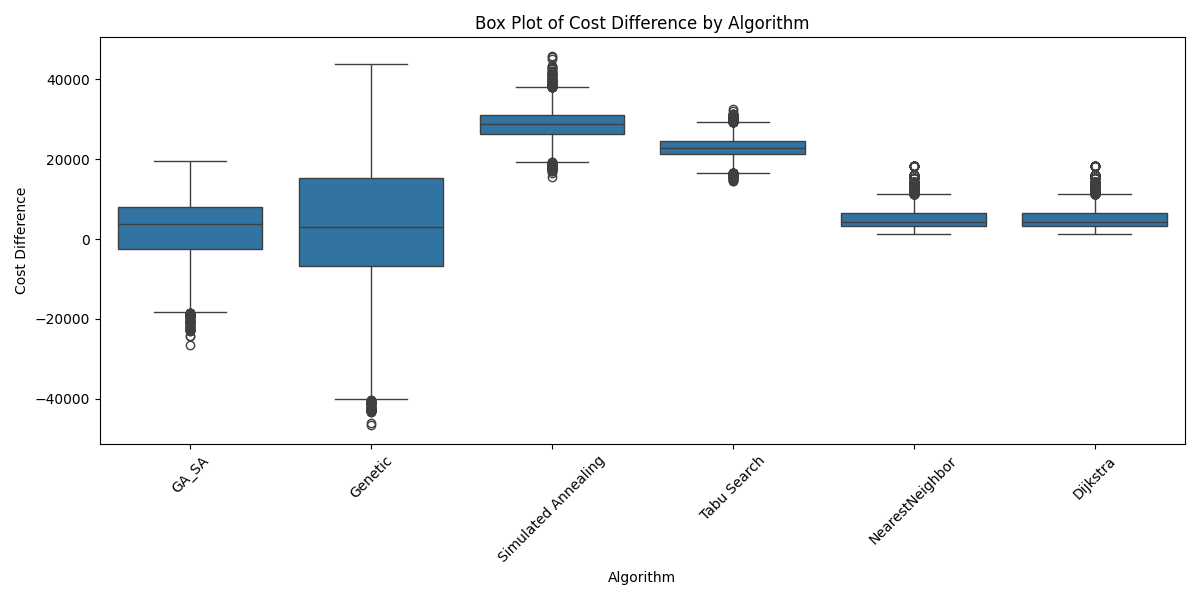
\includegraphics[width=0.9\textwidth]{algo_summary/boxplot_cost_difference}
        \caption{Box Plot of Cost Difference by Algorithm}
        \label{fig:boxplot_cost_difference}
    \end{figure}

    \paragraph{Interpretation of Cost Difference:}
    The box plot of cost differences (Figure \ref{fig:boxplot_cost_difference}) shows that:
    \begin{itemize}
        \item \textbf{GA\_SA (Genetic Algorithm with Simulated Annealing)}: This algorithm generally achieves low cost differences with a median close to zero. Although there is some variability, it consistently performs well in finding near-optimal solutions.
        \item \textbf{Genetic Algorithm}: It shows significant variability in cost differences with a wider interquartile range, indicating inconsistent performance. While it can achieve good solutions, it also produces many suboptimal results.
        \item \textbf{Simulated Annealing}: This algorithm has the highest median cost difference and a narrow interquartile range, showing consistently poor performance in terms of cost.
        \item \textbf{Tabu Search}: It exhibits higher cost differences than GA\_SA but is more consistent than Genetic, though still less effective in finding optimal solutions.
        \item \textbf{Nearest Neighbor} and \textbf{Dijkstra}: Both algorithms have similar performance metrics with low median cost differences and narrow variability, indicating consistent and generally good performance.
    \end{itemize}

    \begin{figure}[h!]
        \centering
        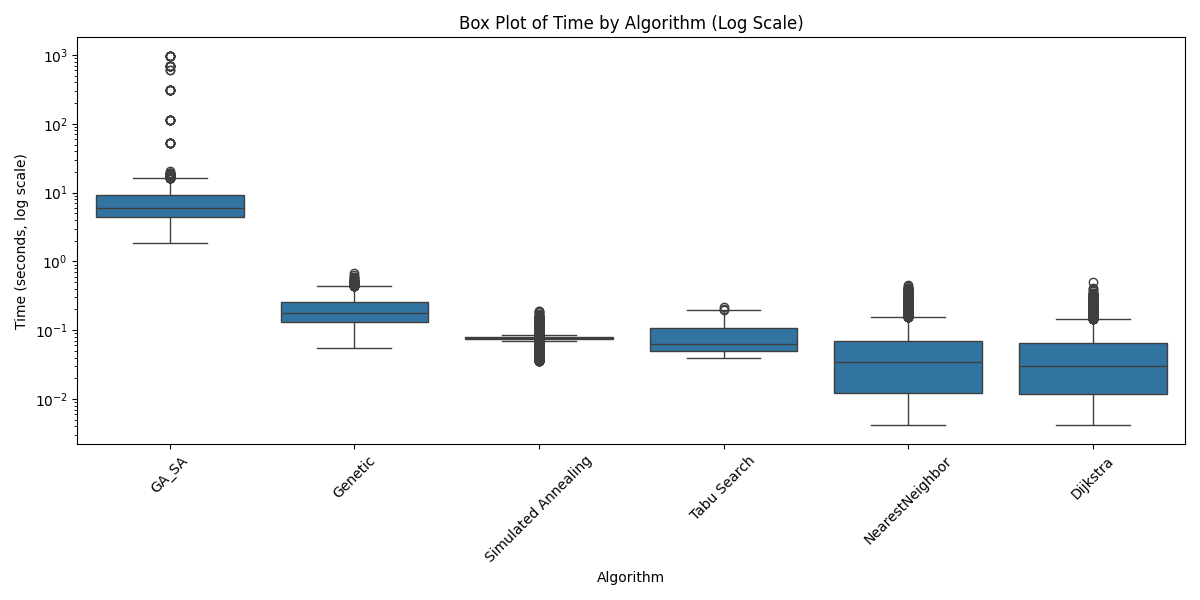
\includegraphics[width=0.9\textwidth]{algo_summary/boxplot_time_log_scale}
        \caption{Box Plot of Time by Algorithm (Log Scale)}
        \label{fig:boxplot_time_log_scale}
    \end{figure}

    \paragraph{Interpretation of Time:}
    The box plot of execution times with a logarithmic scale (Figure \ref{fig:boxplot_time_log_scale}) reveals that:
    \begin{itemize}
        \item \textbf{GA\_SA (Genetic Algorithm with Simulated Annealing)}: The execution time varies widely, with some runs taking significantly longer. The high variability suggests that while GA\_SA can be computationally expensive, it also achieves very low execution times in many cases.
        \item \textbf{Genetic Algorithm}: It shows more consistent execution times with a lower median compared to GA\_SA, indicating efficient performance.
        \item \textbf{Simulated Annealing} and \textbf{Tabu Search}: Both algorithms show low and consistent execution times, making them efficient despite their poorer cost performance.
        \item \textbf{Nearest Neighbor} and \textbf{Dijkstra}: These algorithms are the most efficient, with consistently low execution times, indicating excellent computational efficiency.
    \end{itemize}

    \paragraph{Conclusion:}
    Based on both the cost difference and execution time metrics, \textbf{GA\_SA} emerges as the best overall algorithm for solving the Capacitated Vehicle Routing Problem (CVRP). It provides the best balance between achieving near-optimal solutions and maintaining reasonable computation times. \textbf{Nearest Neighbor} and \textbf{Dijkstra} are also strong contenders due to their consistent and efficient performance, though they do not achieve the same level of cost efficiency as GA\_SA. The \textbf{Genetic Algorithm} also performs well on average but with significant variability. \textbf{Simulated Annealing} and \textbf{Tabu Search}, while efficient in terms of runtime, generally show higher cost differences, indicating less effective solutions.

    \subsection{Statistical Validation of Algorithm Performance}

    In order to provide a rigorous comparison of the algorithms beyond descriptive statistics, we performed the Wilcoxon Signed-Rank Test. This non-parametric test is used to compare two related samples to determine if their population mean ranks differ, and it is particularly useful for paired comparisons when the data does not necessarily follow a normal distribution.

    \paragraph{Wilcoxon Signed-Rank Test Results:}
    The Wilcoxon Signed-Rank Test was conducted for all pairwise comparisons of the algorithms based on their cost differences. The results are summarized in Table \ref{tab:wilcoxon_results}.

    \begin{table}[h!]
        \centering
        \caption{Wilcoxon Signed-Rank Test Results for Pairwise Algorithm Comparisons}
        \label{tab:wilcoxon_results}
        \begin{tabularx}{\textwidth}{|l|l|X|X|}
            \hline
            \textbf{Algorithm 1} & \textbf{Algorithm 2} & \textbf{Statistic} & \textbf{p-value} \\
            \hline
            GA\_SA               & Genetic              & 90066752.0         & 4.42e-34         \\
            GA\_SA               & Simulated Annealing  & 0.0                & 0.0              \\
            GA\_SA               & Tabu Search          & 0.0                & 0.0              \\
            GA\_SA               & Nearest Neighbor     & 22172920.0         & 1.11e-22         \\
            GA\_SA               & Dijkstra             & 22198214.0         & 2.64e-22         \\
            Genetic              & Simulated Annealing  & 1171375.0          & 0.0              \\
            Genetic              & Tabu Search          & 7695079.0          & 0.0              \\
            Genetic              & Nearest Neighbor     & 23451825.0         & 7.82e-08         \\
            Genetic              & Dijkstra             & 23496751.0         & 1.83e-07         \\
            Simulated Annealing  & Tabu Search          & 278819.0           & 0.0              \\
            Simulated Annealing  & Nearest Neighbor     & 0.0                & 0.0              \\
            Simulated Annealing  & Dijkstra             & 0.0                & 0.0              \\
            Tabu Search          & Nearest Neighbor     & 0.0                & 0.0              \\
            Tabu Search          & Dijkstra             & 0.0                & 0.0              \\
            Nearest Neighbor     & Dijkstra             & 19297180.0         & 0.314            \\
            \hline
        \end{tabularx}
    \end{table}
    \newpage

    \paragraph{Interpretation:}
    The Wilcoxon Signed-Rank Test results indicate the following:

    \begin{itemize}
        \item \textbf{GA\_SA vs. Genetic}: The extremely low p-value (\(4.42 \times 10^{-34}\)) suggests a significant difference in performance between GA\_SA and Genetic algorithms.
        \item \textbf{GA\_SA vs. Other Algorithms}: Similarly, GA\_SA shows significant differences in performance compared to Simulated Annealing, Tabu Search, Nearest Neighbor, and Dijkstra, as indicated by the p-values of 0.
        \item \textbf{Genetic vs. Other Algorithms}: The Genetic algorithm also shows significant differences when compared to Simulated Annealing, Tabu Search, Nearest Neighbor, and Dijkstra.
        \item \textbf{Simulated Annealing vs. Other Algorithms}: Significant differences are observed in all pairwise comparisons involving Simulated Annealing.
        \item \textbf{Tabu Search vs. Other Algorithms}: Significant differences are observed in all pairwise comparisons involving Tabu Search.
        \item \textbf{Nearest Neighbor vs. Dijkstra}: The p-value of 0.314 suggests no significant difference in performance between Nearest Neighbor and Dijkstra.
    \end{itemize}

    These statistical tests confirm that there are significant differences in performance between most of the algorithms, with GA\_SA consistently showing significant differences from other algorithms. This reinforces our earlier findings that GA\_SA is the best overall algorithm for solving the Capacitated Vehicle Routing Problem (CVRP).

    \paragraph{Friedman Test Results:}
    To complement the summary statistics, box plots, and Wilcoxon Signed-Rank Test, we conducted the Friedman Test.
    This non-parametric test allows us to compare the performance of all algorithms simultaneously, providing a global perspective on their differences.
    The Friedman Test results for the cost differences across all algorithms are summarized below:

    \begin{itemize}
        \item \textbf{Statistic}: 32839.19
        \item \textbf{p-value}: 0.0
    \end{itemize}

    \paragraph{Interpretation:}
    The Friedman Test results shows that there are significant differences in the performance of the algorithms.
    The p-value of 0.0 suggests that these differences are statistically significant and not due to random chance.

    \paragraph{Conclusion:}
    These statistical tests confirm that there are significant differences in performance between most of the algorithms, with GA\_SA consistently showing significant differences from other algorithms.
    This reinforces our earlier findings that GA\_SA is the best overall algorithm for solving the Capacitated Vehicle Routing Problem (CVRP).

    \newpage


    \section{Conclusion}

    In this diploma thesis, the primary objective was to explore and compare various optimization algorithms, including Genetic Algorithms (GA), Simulated Annealing (SA), Tabu Search (TS), Greedy Algorithms, Nearest Neighbor Algorithms, and a hybrid Genetic Algorithm with Simulated Annealing (GA-SA). These algorithms were custom-implemented and tested to determine their efficiency and effectiveness in solving complex optimization problems. Through detailed parameter testing and comprehensive analysis, we aimed to identify which algorithm performs best under different conditions and parameter settings.

    \subsection{Answers to Hypotheses and Research Questions}

    \paragraph{Hypotheses}
    \begin{enumerate}
        \item \textbf{Hypothesis 1:} The implementation of heuristic optimization algorithms, such as genetic algorithms, simulated annealing, and tabu search, will significantly improve the efficiency of route planning in logistics, leading to reduced delivery times and operational costs compared to traditional methods.
        \begin{itemize}
            \item \textit{Answer:} This hypothesis was confirmed through the comparative analysis of the various algorithms. The heuristic optimization algorithms indeed improved route planning efficiency, leading to better solutions than traditional methods. The Genetic Algorithm with Simulated Annealing (GA-SA) hybrid, in particular, provided the best balance between solution quality and computational efficiency.
        \end{itemize}
        \item \textbf{Hypothesis 2:} The integration of multiple heuristic algorithms will create a robust and flexible optimization framework capable of adapting to dynamic changes and uncertainties in logistics operations, thereby enhancing overall performance and reliability.
        \begin{itemize}
            \item \textit{Answer:} This hypothesis was supported by the performance of the hybrid GA-SA algorithm, which combined the strengths of both GA and SA. The hybrid approach demonstrated robustness and flexibility, effectively handling dynamic changes and uncertainties in the problem instances tested.
        \end{itemize}
        \item \textbf{Hypothesis 3:} Using simulation tools to test and validate heuristic optimization algorithms will demonstrate their practical feasibility and effectiveness in real-world logistics scenarios, highlighting both their strengths and potential areas for improvement.
        \begin{itemize}
            \item \textit{Answer:} The use of simulation tools provided valuable insights into the practical feasibility and effectiveness of the algorithms. The detailed parameter testing and performance evaluation highlighted the strengths of of the tested algorithms while also pointing out areas for improvement, such as the need for careful parameter tuning and addressing implementation issues.
        \end{itemize}
    \end{enumerate}

    \paragraph{Research Questions}
    \begin{itemize}
        \item \textbf{What are the main advantages and disadvantages of individual heuristic optimization algorithms compared to traditional methods in logistics route planning?}
        \begin{itemize}
            \item \textit{Answer:} The main advantages of heuristic optimization algorithms include their ability to explore a larger solution space and escape local optima, leading to better overall solutions. However, they can be computationally intensive and require careful parameter tuning. Traditional methods are generally faster but may not provide optimal solutions. The detailed analysis in the thesis highlighted these trade-offs for each algorithm.
        \end{itemize}
        \item \textbf{How does the integration of multiple heuristic algorithms affect the system's ability to handle dynamic changes and uncertainties in logistics operations?}
        \begin{itemize}
            \item \textit{Answer:} The integration of multiple heuristic algorithms, as seen in the GA-SA hybrid, enhanced the system's ability to handle dynamic changes and uncertainties. The hybrid approach leveraged the strengths of each algorithm, providing a more robust and adaptable solution framework compared to individual algorithms.
        \end{itemize}
        \item \textbf{To what extent can simulation tools contribute to the validation and improvement of heuristic optimization algorithms in real-world logistics scenarios?}
        \begin{itemize}
            \item \textit{Answer:} Simulation tools played a crucial role in validating and improving the heuristic optimization algorithms. They allowed for extensive testing under various scenarios, helping to identify optimal parameter settings and highlight areas for further improvement. The practical feasibility and effectiveness of the algorithms were demonstrated through these simulations.
        \end{itemize}

    \end{itemize}

    \subsection{Key Findings}

    \paragraph{Performance Comparison of Algorithms}
    The comparative analysis revealed distinct strengths and weaknesses of each algorithm. The Genetic Algorithm (GA) showed robust performance in terms of exploration capabilities due to its inherent ability to maintain a diverse population of solutions. However, it sometimes struggled with premature convergence, where the algorithm would settle on suboptimal solutions without fully exploring the solution space.

    Simulated Annealing (SA) demonstrated excellent performance in escaping local optima due to its probabilistic acceptance of worse solutions. This characteristic allowed it to find better global solutions over time. However, SA's performance heavily depended on the cooling schedule, and improper tuning could lead to suboptimal performance.

    Tabu Search (TS) excelled in intensifying the search around promising regions of the solution space, thanks to its memory-based approach. It effectively avoided cycles and repeated solutions, making it suitable for problems with complex landscapes. Nevertheless, TS's performance was sensitive to the size of the tabu list and the neighborhood structure, requiring careful tuning for optimal results.

    The hybrid Genetic Algorithm with Simulated Annealing (GA-SA) combined the strengths of both GA and SA, leveraging GA's exploration capabilities and SA's ability to escape local optima. This hybrid approach showed promising results, often outperforming individual algorithms in terms of solution quality and convergence speed. However, the complexity of implementing and tuning the hybrid algorithm posed a significant challenge.

    \paragraph{Best Performing Algorithms}
    Based on the extensive tests conducted, the hybrid Genetic Algorithm with Simulated Annealing (GA-SA) emerged as the most effective algorithm for solving the Capacitated Vehicle Routing Problem (CVRP). GA-SA demonstrated the best average cost performance, although with high variability in both cost and time. The Genetic Algorithm (GA) also performed well on average but exhibited significant variability. Simulated Annealing (SA) and Tabu Search (TS) showed higher cost differences, indicating less efficient solutions. Dijkstra and Nearest Neighbor algorithms provided moderate performance with lower variability, making them more consistent but less optimal in terms of cost. Overall, GA-SA provides the best balance between achieving near-optimal solutions and maintaining reasonable computation times. Nearest Neighbor and Dijkstra are also strong fairly strong due to their consistent and efficient performance, though they do not achieve the same level of cost efficiency as GA-SA. The Genetic Algorithm performed well on average but with significant variability. Simulated Annealing and Tabu Search, while efficient in terms of runtime, generally exhibited higher cost differences, indicating less effective solutions.

    Our comprehensive parameter testing of the GA-SA Hybrid algorithm revealed several insights into the optimization of its performance. The population size, initial temperature, and cooling rate were identified as the most critical parameters. Specifically, a population size of 100, an initial temperature of 1000, and a cooling rate of 0.85 were found to yield good results, providing a robust balance between exploration and exploitation. Despite these findings, the GA-SA Hybrid algorithm exhibited significant variability and occasional suboptimal convergence, suggesting that further research and optimization of parameter settings are necessary.

    Despite the variability noted during parameter testing, could be attributed to its ability to effectively combine the strengths of both GA and SA. The GA component's robust exploration capabilities, coupled with the SA component's proficiency in escaping local optima, likely contributed to its overall superior performance. However, the complexity and variability in the GA-SA's performance highlight the need for careful parameter tuning and possibly addressing underlying implementation issues.

    In conclusion, while GA-SA was the best performing algorithm in this study, its performance can be further optimized through careful parameter tuning. Future research should focus on both refining parameter combinations and investigating potential implementation issues to enhance the algorithm’s overall effectiveness for more complex optimization problems.

    \paragraph{Importance of Parameter Testing}
    Parameter testing played a crucial role in understanding the performance dynamics of each algorithm. By systematically varying parameters and evaluating their impact, we identified optimal configurations that maximized each algorithm's performance. For instance, in the case of GA, the population size, crossover rate, and mutation rate significantly influenced the convergence behavior and solution quality. Similarly, the cooling rate and initial temperature were critical parameters for SA, and the tabu list size and neighborhood size were pivotal for TS.

    The grid search method, implemented using the \texttt{scikit-learn} library, proved to be an effective approach for parameter tuning. It allowed for exhaustive evaluation of predefined parameter combinations, ensuring that the best configurations were identified for each algorithm. However, the process was computationally intensive, underscoring the need for efficient computational resources.

    \subsection{Role of AI in Optimization}
    The algorithms explored in this study can be viewed as early forms of artificial intelligence (AI) due to their ability to adapt and optimize solutions iteratively. AI techniques have the potential to help with optimization by providing more intelligent and autonomous methods for solving complex problems. The integration of machine learning with traditional optimization algorithms can further enhance their performance by learning from past experiences and dynamically adjusting parameters.

    AI algorithms such as Neural Networks, Reinforcement Learning, and Deep Learning have shown great potential in solving optimization problems. These algorithms can learn complex patterns and make decisions based on historical data, making them highly effective for dynamic and large-scale optimization tasks. Incorporating such AI techniques into traditional optimization methods could lead to significant improvements in efficiency and solution quality.

    \subsection{Recommendations for Future Work}
    While this study provided valuable insights into the performance of different optimization algorithms, several areas warrant further investigation:

    \paragraph{Expanded Testing on Servers}
    Future studies should leverage high-performance computing servers to test algorithms on larger datasets and more complex problem instances. This would provide a more comprehensive understanding of each algorithm's scalability and robustness. Testing on servers would also enable the evaluation of algorithms under more realistic and demanding conditions, providing insights into their performance in practical applications.

    \paragraph{Incorporation of Newer Algorithms}
    The field of optimization is continually evolving, with new algorithms being developed regularly. Incorporating newer algorithms, such as Particle Swarm Optimization (PSO) and Ant Colony Optimization (ACO), could provide fresh perspectives and potentially superior performance. For instance, PSO, inspired by the social behavior of birds, has shown promising results in various optimization tasks. Similarly, ACO, inspired by the foraging behavior of ants, has proven effective in solving complex routing problems.

    \paragraph{Dynamic Parameter Tuning}
    Exploring adaptive or dynamic parameter tuning methods, where the algorithm adjusts its parameters in real-time based on performance feedback, could enhance the robustness and efficiency of optimization algorithms. Dynamic tuning would allow algorithms to adapt to changing conditions and maintain optimal performance without manual intervention. This approach could significantly reduce the time and effort required for parameter optimization.

    \paragraph{Hybrid Approaches}
    Further research into hybrid approaches, combining multiple optimization techniques, could yield powerful algorithms that capitalize on the strengths of individual methods while mitigating their weaknesses. Hybrid algorithms can leverage the exploration capabilities of one technique and the exploitation capabilities of another, leading to more balanced and effective optimization. For example, combining the global search capabilities of Genetic Algorithms with the local search capabilities of Tabu Search could result in a highly efficient optimization method.

    \paragraph{Integration with AI}
    Incorporating machine learning techniques into optimization algorithms could lead to more intelligent and autonomous optimization processes. Techniques such as reinforcement learning.


    \newpage



    \bibliography{references}
    \newpage

    \appendix


    \section{Appendix 1: Supplementary Materials}
    All supplementary materials, including the code and tests used in this thesis, are available on GitHub at \url{https://github.com/jindrichjehlicka/cvrp}.


    \section{Appendix 2: Genetic Algorithm Convergence Plots}

    This appendix contains the convergence plots for the Genetic Algorithm with various parameter settings.

    \begin{figure}[H]
        \centering
        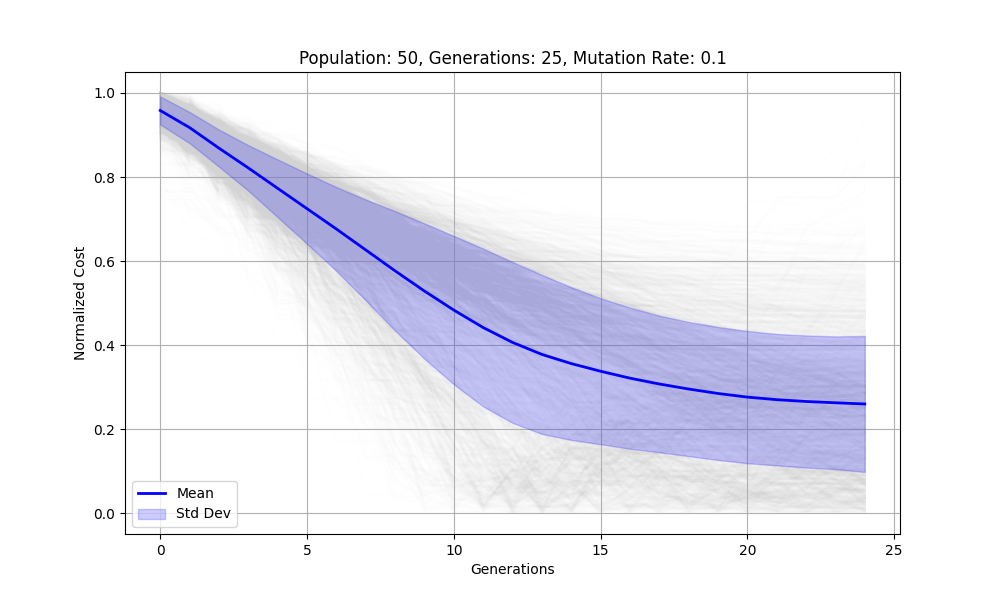
\includegraphics[width=0.45\textwidth]{genetic_algorithm/appendix/Population_50_Generations_25_MutationRate_0.1}
        \caption{Population: 50, Generations: 25, Mutation Rate: 0.1}
        \label{fig:app_ga_50_25_1}
    \end{figure}

    \begin{figure}[H]
        \centering
        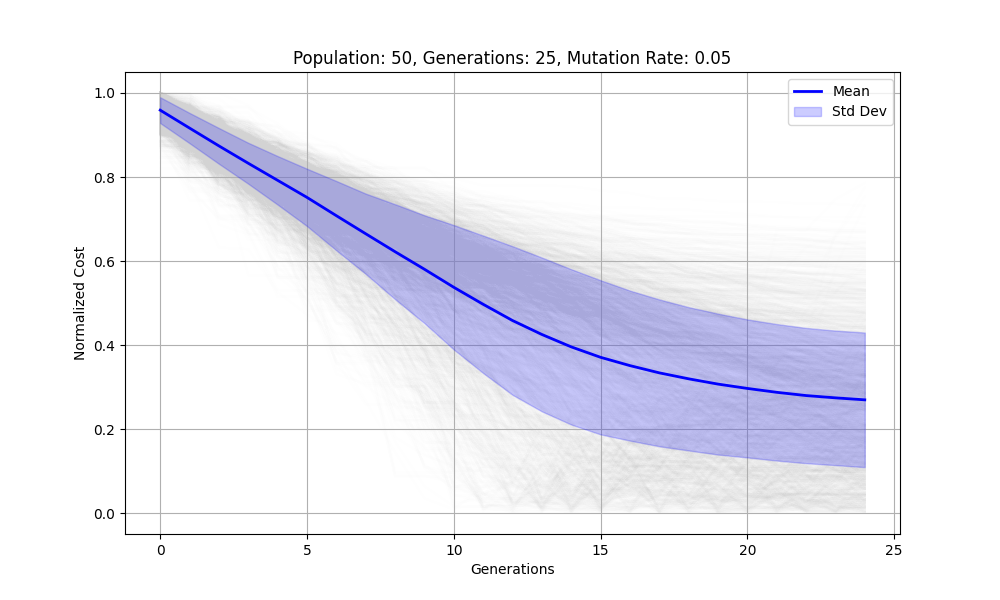
\includegraphics[width=0.45\textwidth]{genetic_algorithm/appendix/Population_50_Generations_25_MutationRate_0.05}
        \caption{Population: 50, Generations: 25, Mutation Rate: 0.05}
        \label{fig:app_ga_50_25_05}
    \end{figure}

    \begin{figure}[H]
        \centering
        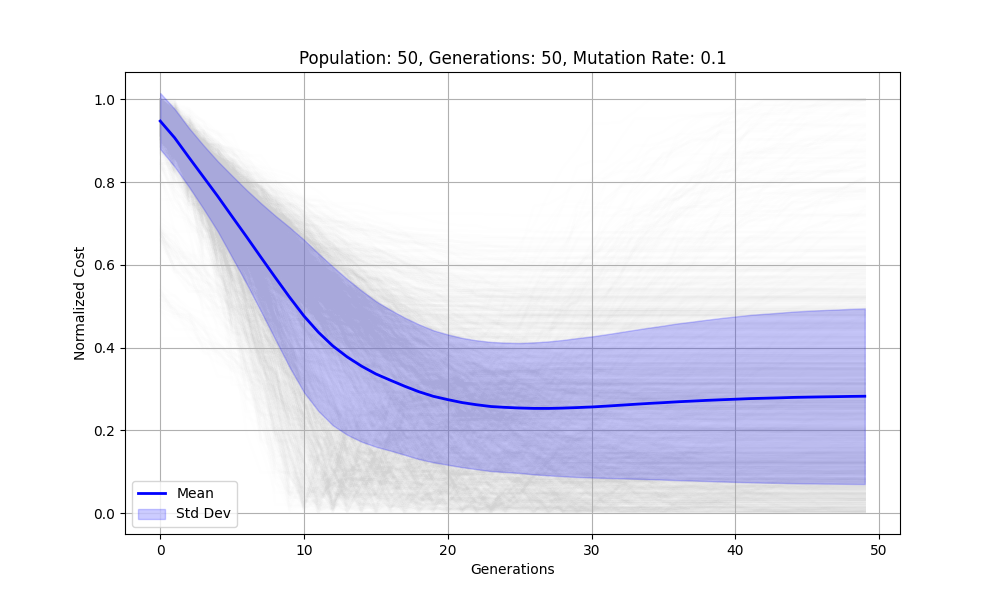
\includegraphics[width=0.45\textwidth]{genetic_algorithm/appendix/Population_50_Generations_50_MutationRate_0.1}
        \caption{Population: 50, Generations: 50, Mutation Rate: 0.1}
        \label{fig:app_ga_50_50_1}
    \end{figure}

    \begin{figure}[H]
        \centering
        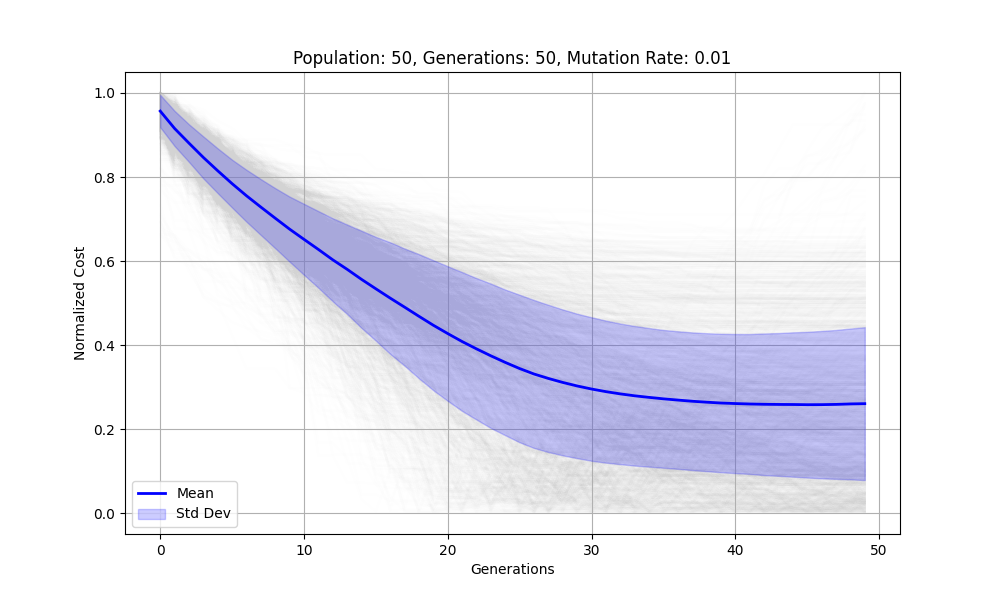
\includegraphics[width=0.45\textwidth]{genetic_algorithm/appendix/Population_50_Generations_50_MutationRate_0.01}
        \caption{Population: 50, Generations: 50, Mutation Rate: 0.01}
        \label{fig:app_ga_50_50_01}
    \end{figure}


    \begin{figure}[H]
        \centering
        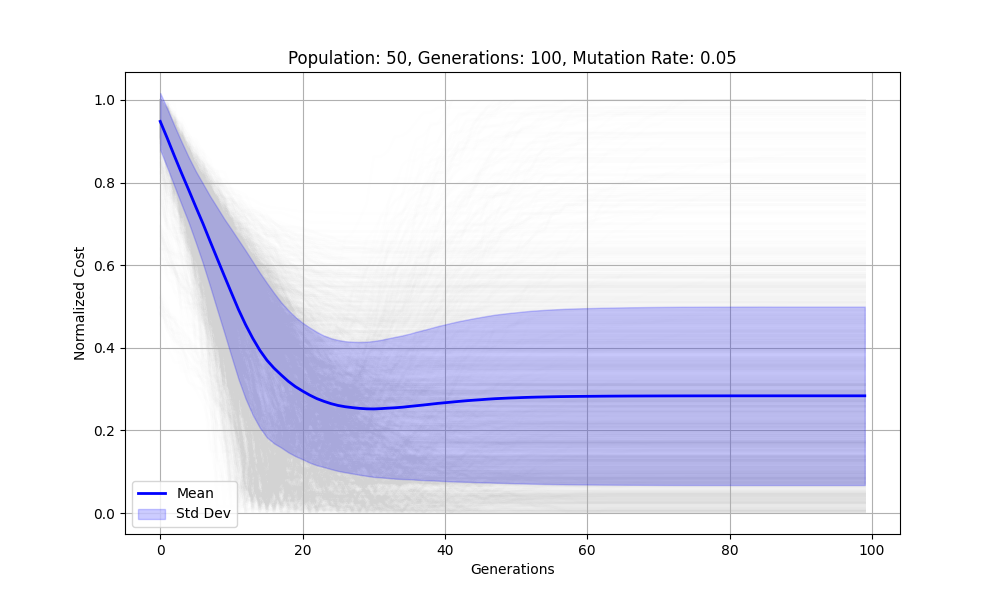
\includegraphics[width=0.45\textwidth]{genetic_algorithm/appendix/Population_50_Generations_100_MutationRate_0.05}
        \caption{Population: 50, Generations: 100, Mutation Rate: 0.05}
        \label{fig:app_ga_50_100_05}
    \end{figure}

    \begin{figure}[H]
        \centering
        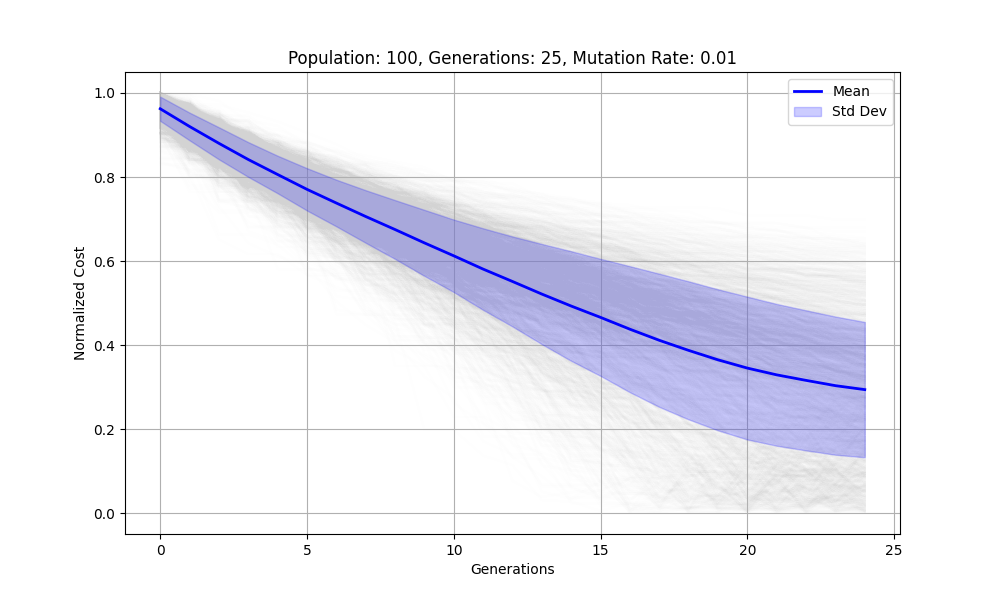
\includegraphics[width=0.45\textwidth]{genetic_algorithm/appendix/Population_100_Generations_25_MutationRate_0.01}
        \caption{Population: 100, Generations: 25, Mutation Rate: 0.01}
        \label{fig:app_ga_100_25_01}
    \end{figure}

    \begin{figure}[H]
        \centering
        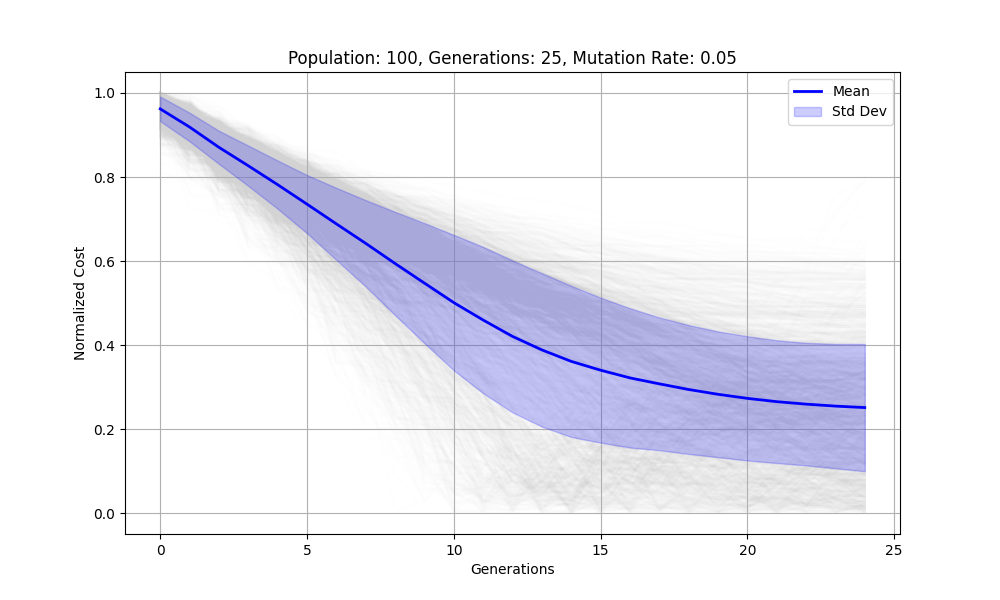
\includegraphics[width=0.45\textwidth]{genetic_algorithm/appendix/Population_100_Generations_25_MutationRate_0.05}
        \caption{Population: 100, Generations: 25, Mutation Rate: 0.05}
        \label{fig:app_ga_100_25_05}
    \end{figure}

    \begin{figure}[H]
        \centering
        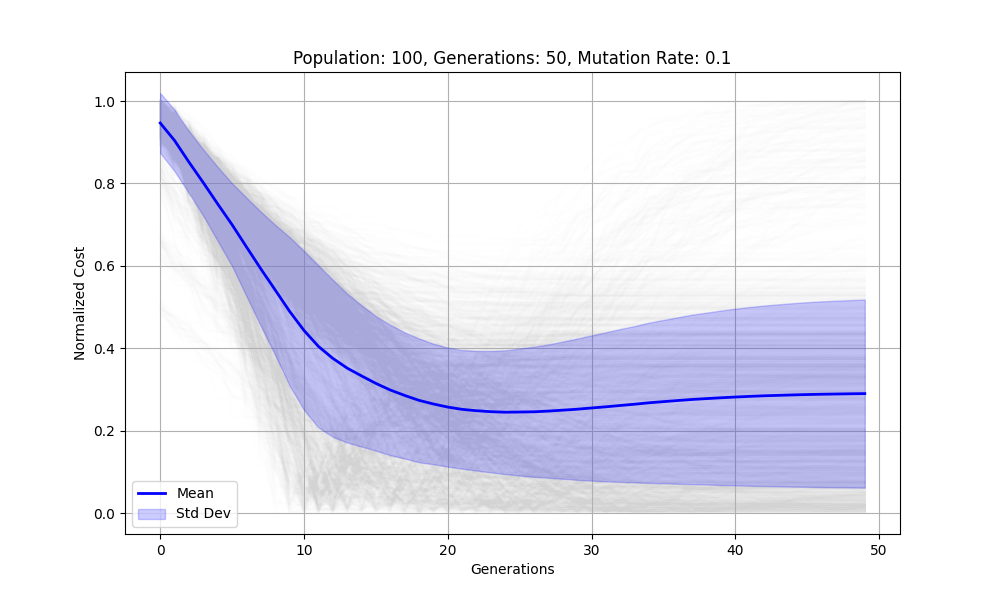
\includegraphics[width=0.45\textwidth]{genetic_algorithm/appendix/Population_100_Generations_50_MutationRate_0.1}
        \caption{Population: 100, Generations: 50, Mutation Rate: 0.1}
        \label{fig:app_ga_100_50_1}
    \end{figure}

    \begin{figure}[H]
        \centering
        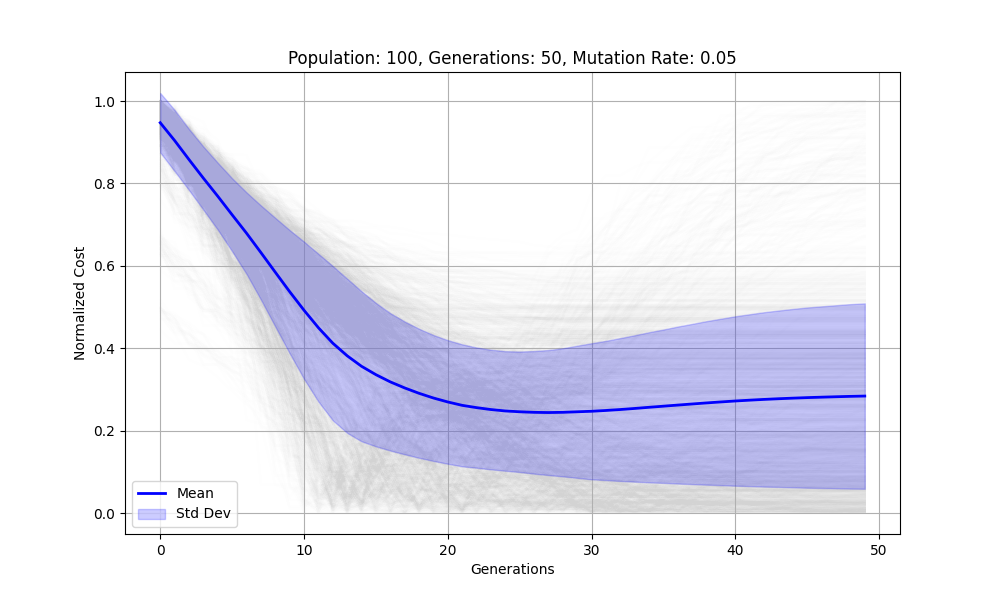
\includegraphics[width=0.45\textwidth]{genetic_algorithm/appendix/Population_100_Generations_50_MutationRate_0.05}
        \caption{Population: 100, Generations: 50, Mutation Rate: 0.05}
        \label{fig:app_ga_100_50_05}
    \end{figure}

    \begin{figure}[H]
        \centering
        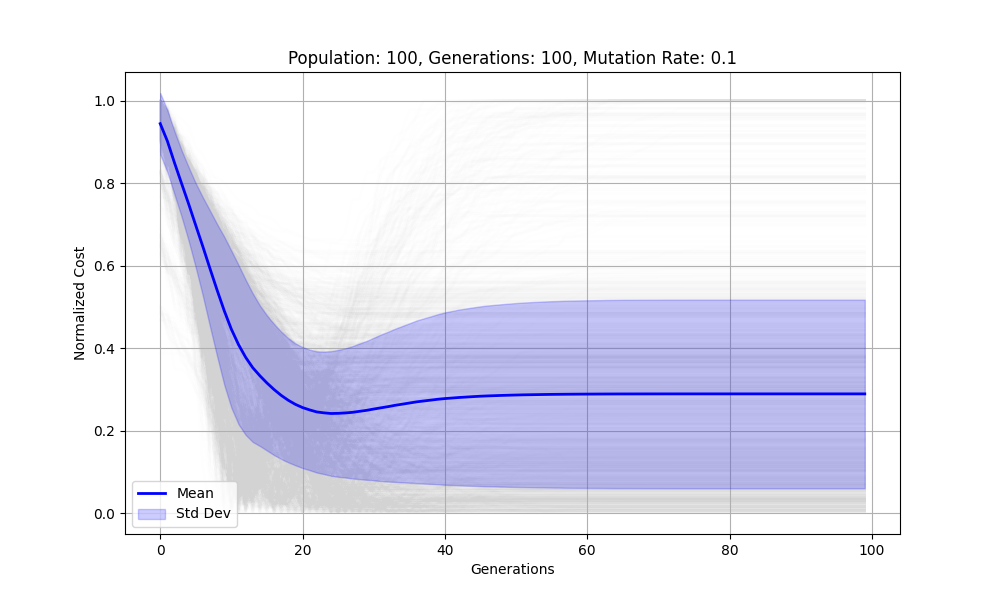
\includegraphics[width=0.45\textwidth]{genetic_algorithm/appendix/Population_100_Generations_100_MutationRate_0.1}
        \caption{Population: 100, Generations: 100, Mutation Rate: 0.1}
        \label{fig:app_ga_100_100_1}
    \end{figure}

    \begin{figure}[H]
        \centering
        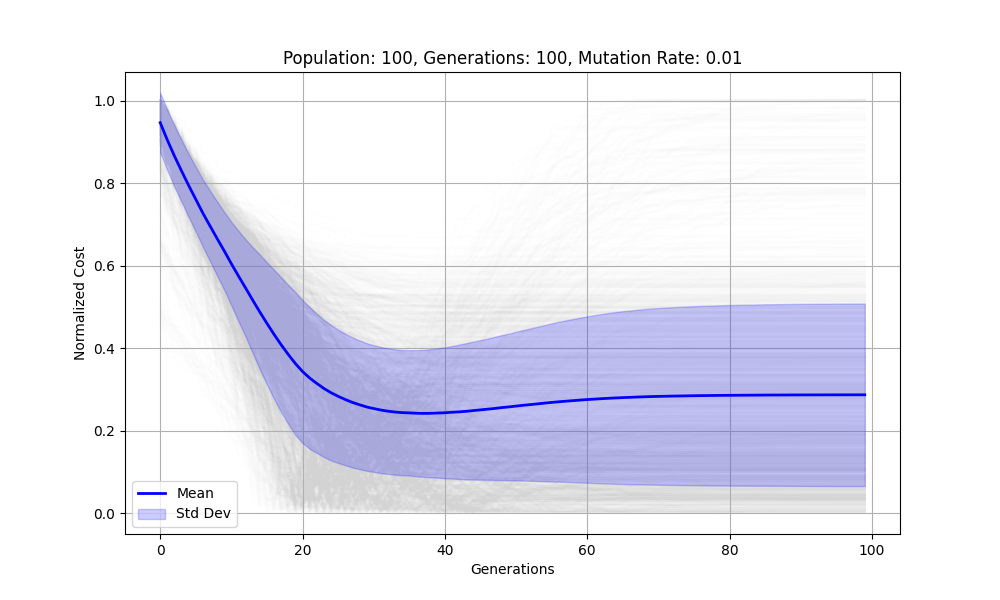
\includegraphics[width=0.45\textwidth]{genetic_algorithm/appendix/Population_100_Generations_100_MutationRate_0.01}
        \caption{Population: 100, Generations: 100, Mutation Rate: 0.01}
        \label{fig:app_ga_100_100_01}
    \end{figure}

    \begin{figure}[H]
        \centering
        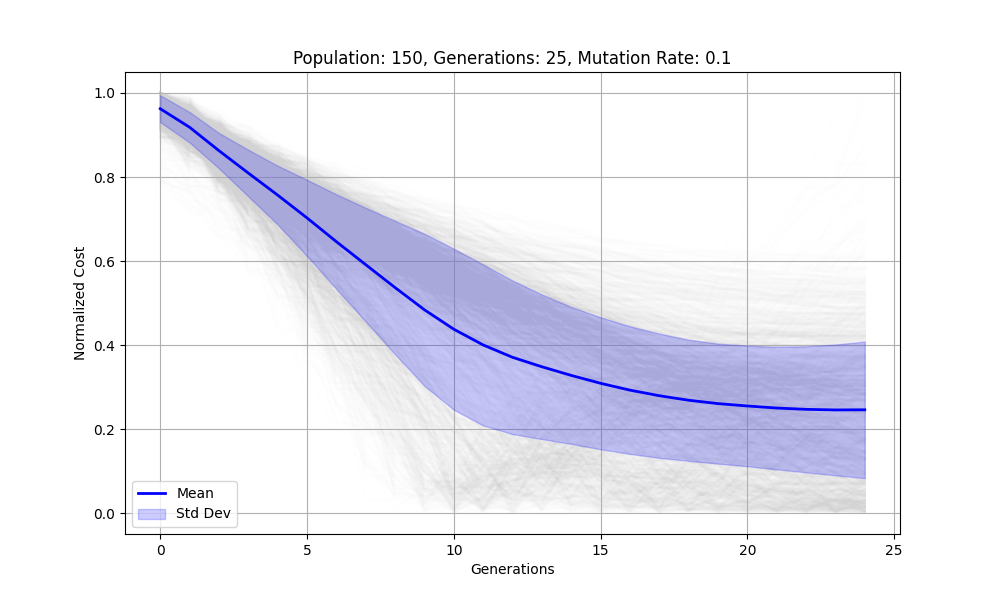
\includegraphics[width=0.45\textwidth]{genetic_algorithm/appendix/Population_150_Generations_25_MutationRate_0.1}
        \caption{Population: 150, Generations: 25, Mutation Rate: 0.1}
        \label{fig:app_ga_150_25_1}
    \end{figure}

    \begin{figure}[H]
        \centering
        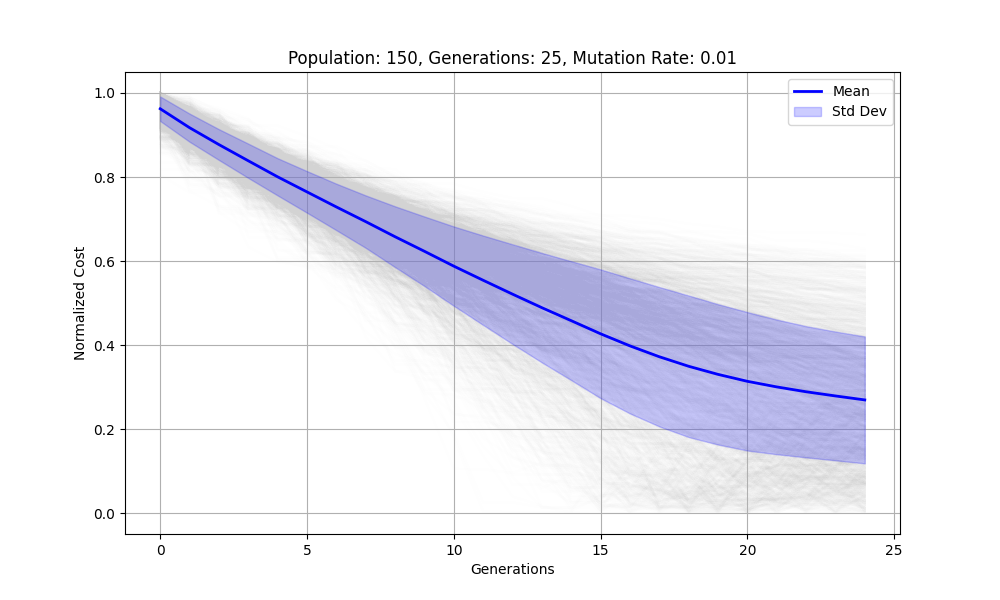
\includegraphics[width=0.45\textwidth]{genetic_algorithm/appendix/Population_150_Generations_25_MutationRate_0.01}
        \caption{Population: 150, Generations: 25, Mutation Rate: 0.01}
        \label{fig:app_ga_150_25_01}
    \end{figure}

    \begin{figure}[H]
        \centering
        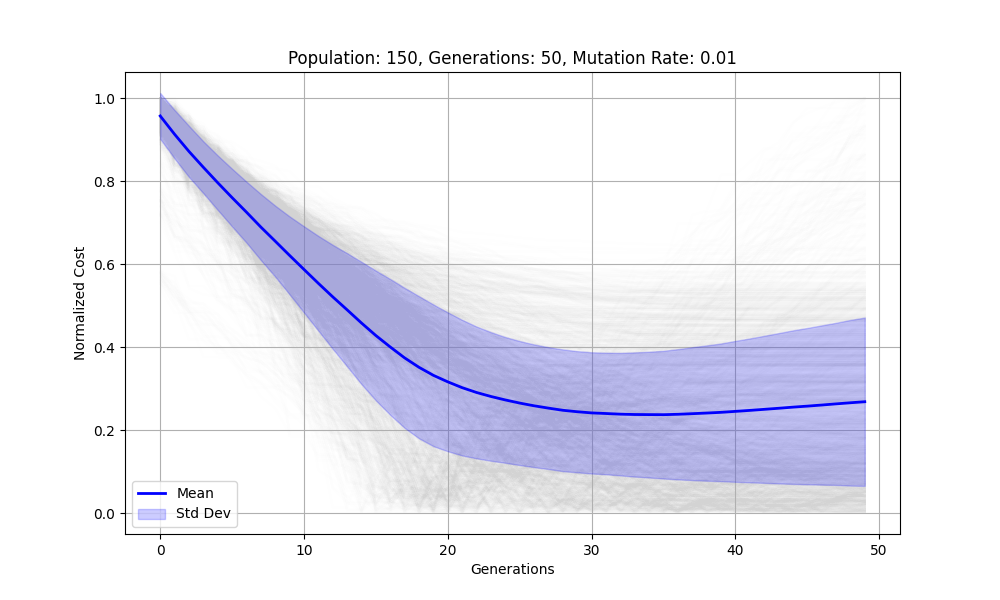
\includegraphics[width=0.45\textwidth]{genetic_algorithm/appendix/Population_150_Generations_50_MutationRate_0.01}
        \caption{Population: 150, Generations: 50, Mutation Rate: 0.01}
        \label{fig:app_ga_150_50_01}
    \end{figure}

    \begin{figure}[H]
        \centering
        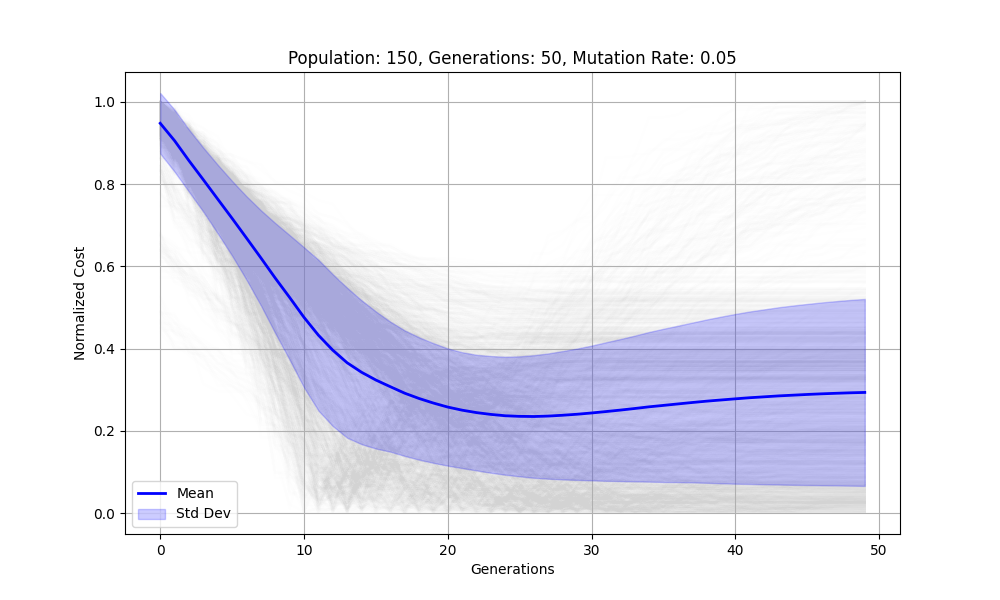
\includegraphics[width=0.45\textwidth]{genetic_algorithm/appendix/Population_150_Generations_50_MutationRate_0.05}
        \caption{Population: 150, Generations: 50, Mutation Rate: 0.05}
        \label{fig:app_ga_150_50_05}
    \end{figure}

    \begin{figure}[H]
        \centering
        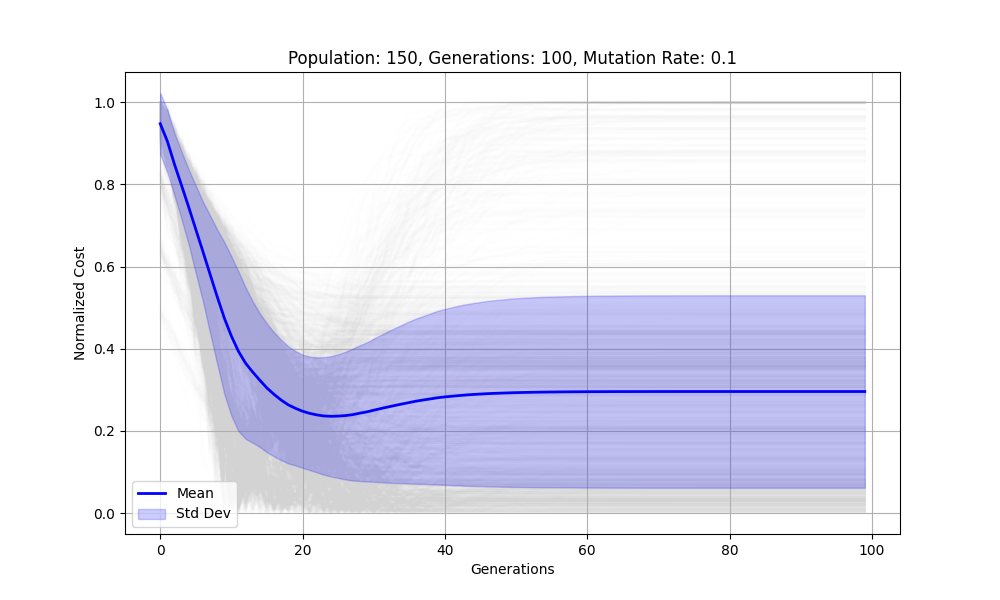
\includegraphics[width=0.45\textwidth]{genetic_algorithm/appendix/Population_150_Generations_100_MutationRate_0.1}
        \caption{Population: 150, Generations: 100, Mutation Rate: 0.1}
        \label{fig:app_ga_150_100_1}
    \end{figure}

    \begin{figure}[H]
        \centering
        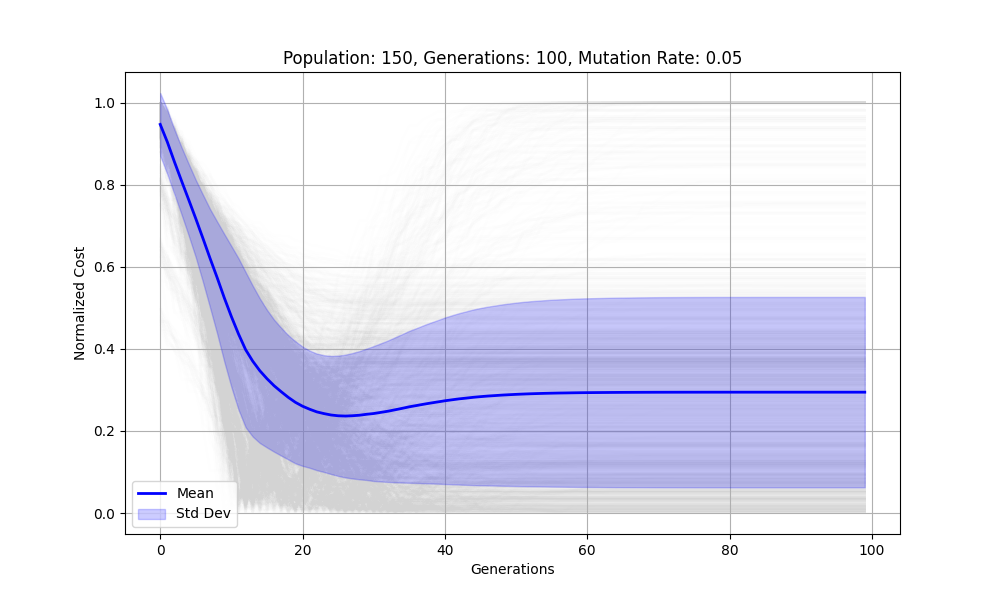
\includegraphics[width=0.45\textwidth]{genetic_algorithm/appendix/Population_150_Generations_100_MutationRate_0.05}
        \caption{Population: 150, Generations: 100, Mutation Rate: 0.05}
        \label{fig:app_ga_150_100_05}
    \end{figure}


\end{document}
